\documentclass[aspectratio=169,10pt]{beamer}

\usetheme{default}
\usefonttheme{professionalfonts}
\setbeamertemplate{navigation symbols}{}
\setbeamersize{text margin left=0.70cm,text margin right=0.70cm}

\usepackage[T1]{fontenc}
\usepackage{array}
\usepackage{booktabs}
\usepackage{colortbl}
\usepackage{graphicx}
\usepackage{tikz}
\usepackage{xspace}
\usetikzlibrary{arrows.meta,positioning}

% Compile from either pmds/latex or the repository root.
\graphicspath{{../results/final_clean_results/plots/}{pmds/results/final_clean_results/plots/}}

\definecolor{Ink}{HTML}{17212B}
\definecolor{Muted}{HTML}{66717D}
\definecolor{Paper}{HTML}{F7F9FA}
\definecolor{Line}{HTML}{D9E0E5}
\definecolor{Teal}{HTML}{087E8B}
\definecolor{TealLight}{HTML}{DCEFF0}
\definecolor{Coral}{HTML}{D95D39}
\definecolor{CoralLight}{HTML}{F8E4DE}
\definecolor{Gold}{HTML}{C58B13}
\definecolor{GoldLight}{HTML}{F6ECD2}
\definecolor{Green}{HTML}{2E7D5B}
\definecolor{GreenLight}{HTML}{DDEEE6}
\definecolor{Purple}{HTML}{6C5B8C}
\definecolor{PurpleLight}{HTML}{E8E2F1}
\definecolor{GrayLight}{HTML}{E9EEF1}

\setbeamercolor{normal text}{fg=Ink,bg=white}
\setbeamercolor{frametitle}{fg=Ink}
\setbeamercolor{structure}{fg=Teal}
\setbeamercolor{itemize item}{fg=Teal}
\setbeamercolor{itemize subitem}{fg=Teal}
\setbeamerfont{frametitle}{size=\Large,series=\bfseries}
\setbeamerfont{footline}{size=\scriptsize}

\setbeamertemplate{frametitle}{
  \vspace{0.24cm}
  \insertframetitle\par
  \vspace{0.08cm}
  {\color{Teal}\rule{\linewidth}{0.7pt}}
}
\setbeamertemplate{footline}{
  \leavevmode
  \hbox to \paperwidth{%
    \hspace{0.70cm}%
    {\usebeamerfont{footline}\color{Muted}Amirhossein Bagheri}%
    \hfill
    {\usebeamerfont{footline}\color{Muted}PMDS Final Clean Benchmark
      \quad \insertframenumber/\inserttotalframenumber}%
    \hspace{0.40cm}%
  }
  \vspace{0.18cm}
}
\setbeamertemplate{itemize item}{\raise0.2ex\hbox{\small$\blacktriangleright$}}
\setbeamertemplate{itemize subitem}{\raise0.2ex\hbox{\scriptsize$\bullet$}}

\newcommand{\system}{\textsc{PMDS Forecasting Project}\xspace}
\newcommand{\key}[1]{{\color{Teal}\textbf{#1}}}
\newcommand{\tagbox}[2]{%
  \tikz[baseline=(tag.base)]{
    \node[fill=#1,rounded corners=1.5pt,inner xsep=6pt,inner ysep=3pt]
      (tag) {\strut #2};
  }%
}
\newcommand{\widebox}[2]{%
  \tikz{%
    \node[fill=#1,rounded corners=1.5pt,inner xsep=5pt,inner ysep=4pt,
      text width=0.89\linewidth,align=center] {#2};%
  }%
}
\newcommand{\winnerbox}[2]{%
  \colorbox{#1}{%
    \parbox[c][0.77cm][c]{0.91\linewidth}{\centering\scriptsize\textbf{#2}}%
  }%
}
\newcolumntype{L}[1]{>{\raggedright\arraybackslash}p{#1}}
\newcolumntype{C}[1]{>{\centering\arraybackslash}p{#1}}

\title{\system: Foundation Models for Time-Series Forecasting}
\author{Amirhossein Bagheri}
\institute{Politecnico di Milano \qquad Supervisor: Tommaso Bianchi}
\date{}

\begin{document}

% ------------------------------------------------------------
\begin{frame}[plain]
  \vspace{0.45cm}
  {\color{Teal}\rule{1.25cm}{3pt}}

  \vspace{0.42cm}
  {\fontsize{25}{30}\selectfont\bfseries
    Time-Series Foundation Models\\
    Under a Common Forecasting Benchmark\par}

  \vspace{0.30cm}
  {\Large\color{Muted}
    Chronos T5, TimesFM 2.5, and Moirai 2.0\\
    against established forecasting baselines\par}

  \vspace{0.46cm}
  \tagbox{TealLight}{\small\textbf{12 models}}
  \hspace{0.16cm}
  \tagbox{GreenLight}{\small\textbf{12 datasets}}
  \hspace{0.16cm}
  \tagbox{GoldLight}{\small\textbf{5 core metrics}}

  \vfill
  {\small\color{Muted}Prepared by}\par
  \vspace{0.06cm}
  {\large\bfseries Amirhossein Bagheri}

  \vspace{0.16cm}
  {\small\color{Muted}
    Politecnico di Milano \qquad Supervisor: Tommaso Bianchi}
\end{frame}

% ------------------------------------------------------------
\begin{frame}{Benchmark question and model lineup}
  \vspace{0.10cm}
  \begin{center}
    \begin{minipage}{0.91\linewidth}
      \Large\raggedright
      How do pretrained \key{time-series foundation models} compare with
      statistical, neural, and seasonal baselines when every model receives
      the same context, forecast horizon, rolling origins, and metrics?
    \end{minipage}
  \end{center}

  \vspace{0.45cm}
  \begin{columns}[T,totalwidth=0.96\linewidth]
    \begin{column}{0.30\linewidth}
      \tagbox{TealLight}{\textbf{Foundation models}}
      \vspace{0.18cm}
      \small
      \begin{itemize}
        \item Chronos T5 Tiny
        \item TimesFM 2.5 200M
        \item Moirai 2.0 Small
      \end{itemize}
    \end{column}
    \begin{column}{0.30\linewidth}
      \tagbox{GoldLight}{\textbf{Comparison models}}
      \vspace{0.18cm}
      \small
      \begin{itemize}
        \item ARIMA and AutoARIMA
        \item Prophet and DeepAR
        \item Seasonal Naive
      \end{itemize}
    \end{column}
    \begin{column}{0.30\linewidth}
      \tagbox{GreenLight}{\textbf{Chronos scale study}}
      \vspace{0.18cm}
      \small
      \begin{itemize}
        \item Mini, Small
        \item Base, Large
        \item Same 12 datasets
      \end{itemize}
    \end{column}
  \end{columns}
\end{frame}

\section{Foundation-Model Architectures}

% ------------------------------------------------------------
\begin{frame}{Chronos T5: real values become language tokens}
  \vspace{0.10cm}
  \begin{center}
    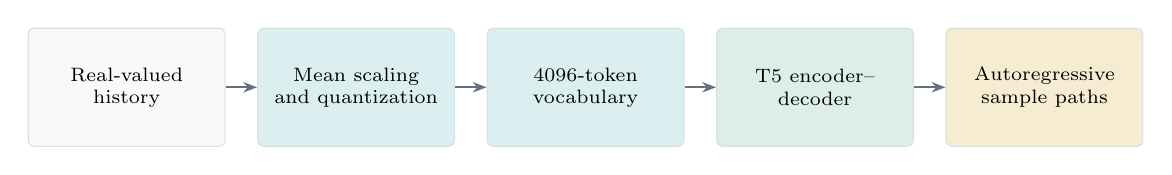
\begin{tikzpicture}[
      node distance=4mm,
      box/.style={draw=Line,rounded corners=2pt,align=center,
        minimum width=25mm,minimum height=15mm,font=\scriptsize},
      arrow/.style={-{Stealth[length=5pt]},thick,color=Muted}
    ]
      \node[box,fill=Paper] (series) {Real-valued\\history};
      \node[box,fill=TealLight,right=of series] (scale) {Mean scaling\\and quantization};
      \node[box,fill=TealLight,right=of scale] (tokens) {4096-token\\vocabulary};
      \node[box,fill=GreenLight,right=of tokens] (t5) {T5 encoder--\\decoder};
      \node[box,fill=GoldLight,right=of t5] (samples) {Autoregressive\\sample paths};
      \draw[arrow] (series) -- (scale);
      \draw[arrow] (scale) -- (tokens);
      \draw[arrow] (tokens) -- (t5);
      \draw[arrow] (t5) -- (samples);
    \end{tikzpicture}
  \end{center}

  \vspace{0.48cm}
  \begin{columns}[T,totalwidth=0.92\linewidth]
    \begin{column}{0.42\linewidth}
      \small
      \tagbox{TealLight}{\textbf{Training representation}}
      \vspace{0.14cm}
      \begin{itemize}
        \item Scale each series by its absolute mean.
        \item Quantize scaled values into uniformly spaced bins.
        \item Train with categorical cross-entropy like a language model.
      \end{itemize}
    \end{column}
    \begin{column}{0.42\linewidth}
      \small
      \tagbox{GoldLight}{\textbf{Probabilistic inference}}
      \vspace{0.14cm}
      \begin{itemize}
        \item Sample future tokens autoregressively.
        \item Map tokens back to numerical trajectories.
        \item Derive median and quantiles from multiple paths.
      \end{itemize}
    \end{column}
  \end{columns}

  \vfill
  {\tiny\color{Muted}Source: Ansari et al., \emph{Chronos: Learning the Language of Time Series}, TMLR 2024; official Amazon model card.}
\end{frame}

% ------------------------------------------------------------
\begin{frame}{Chronos T5: one architecture evaluated at five scales}
  \vspace{0.06cm}
  \begin{columns}[T,totalwidth=0.95\linewidth]
    \begin{column}{0.51\linewidth}
      \small
      \renewcommand{\arraystretch}{1.25}
      \setlength{\tabcolsep}{4pt}
      \begin{tabular}{L{0.44\linewidth} C{0.22\linewidth} C{0.24\linewidth}}
        \toprule
        \textbf{Checkpoint} & \textbf{Params.} & \textbf{Execution} \\
        \midrule
        Chronos T5 Tiny  & $\sim$8M   & CPU / FP32 \\
        Chronos T5 Mini  & $\sim$20M  & GPU / BF16 \\
        Chronos T5 Small & $\sim$46M  & GPU / BF16 \\
        Chronos T5 Base  & $\sim$200M & GPU / BF16 \\
        Chronos T5 Large & $\sim$710M & GPU / BF16 \\
        \bottomrule
      \end{tabular}
    \end{column}
    \begin{column}{0.38\linewidth}
      \small
      \tagbox{GreenLight}{\textbf{Benchmark generation}}
      \vspace{0.18cm}
      \begin{itemize}
        \item 100 sample paths per forecast
        \item Three seeded repetitions
        \item Temperature 1.0
        \item Top-$k$ 50, top-$p$ 1.0
        \item Median used for point metrics
      \end{itemize}
    \end{column}
  \end{columns}

  \vspace{0.45cm}
  \centering
  \widebox{TealLight}{\small Scaling the checkpoint changes capacity and compute, not the tokenization or forecasting objective.}

  \vfill
  {\tiny\color{Muted}Checkpoint sizes: official Amazon Chronos model cards. Execution settings: PMDS final-clean configurations.}
\end{frame}

% ------------------------------------------------------------
\begin{frame}{TimesFM 2.5: a patched decoder-only Transformer}
  \vspace{0.08cm}
  \begin{center}
    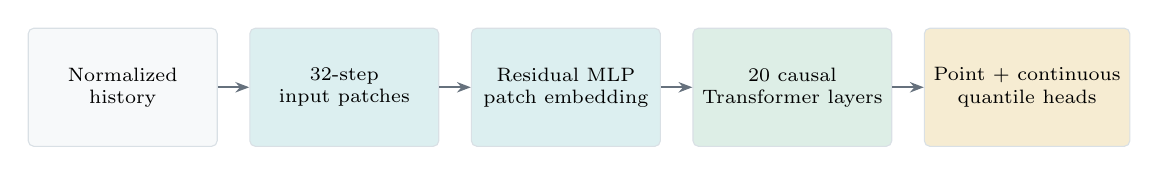
\begin{tikzpicture}[
      node distance=4mm,
      box/.style={draw=Line,rounded corners=2pt,align=center,
        minimum width=24mm,minimum height=15mm,font=\scriptsize},
      arrow/.style={-{Stealth[length=5pt]},thick,color=Muted}
    ]
      \node[box,fill=Paper] (series) {Normalized\\history};
      \node[box,fill=TealLight,right=of series] (patch) {32-step\\input patches};
      \node[box,fill=TealLight,right=of patch] (mlp) {Residual MLP\\patch embedding};
      \node[box,fill=GreenLight,right=of mlp] (decoder) {20 causal\\Transformer layers};
      \node[box,fill=GoldLight,right=of decoder] (head) {Point + continuous\\quantile heads};
      \draw[arrow] (series) -- (patch);
      \draw[arrow] (patch) -- (mlp);
      \draw[arrow] (mlp) -- (decoder);
      \draw[arrow] (decoder) -- (head);
    \end{tikzpicture}
  \end{center}

  \vspace{0.46cm}
  \begin{columns}[T,totalwidth=0.92\linewidth]
    \begin{column}{0.42\linewidth}
      \small
      \tagbox{GreenLight}{\textbf{200M checkpoint}}
      \vspace{0.14cm}
      \begin{itemize}
        \item 20 decoder layers
        \item 16 attention heads
        \item Model dimension 1280
        \item Causal attention across patches
      \end{itemize}
    \end{column}
    \begin{column}{0.42\linewidth}
      \small
      \tagbox{GoldLight}{\textbf{Multi-step decoding}}
      \vspace{0.14cm}
      \begin{itemize}
        \item Predicts 128 future steps per output patch.
        \item Longer horizons are generated recursively.
        \item Version 2.5 provides native continuous quantiles.
      \end{itemize}
    \end{column}
  \end{columns}

  \vfill
  {\tiny\color{Muted}Sources: Das et al., \emph{A Decoder-Only Foundation Model for Time-Series Forecasting}, ICML 2024; official TimesFM 2.5 implementation.}
\end{frame}

% ------------------------------------------------------------
\begin{frame}{TimesFM 2.5 in this benchmark}
  \vspace{0.08cm}
  \begin{columns}[T,totalwidth=0.94\linewidth]
    \begin{column}{0.43\linewidth}
      \tagbox{GreenLight}{\textbf{Input handling}}
      \vspace{0.20cm}
      \small
      \begin{itemize}
        \item Maximum benchmark context: 512
        \item Input normalization enabled
        \item Context compiled to the smallest 32-step-aligned bucket
        \item No dataset-specific fine-tuning
      \end{itemize}
    \end{column}
    \begin{column}{0.43\linewidth}
      \tagbox{GoldLight}{\textbf{Output handling}}
      \vspace{0.20cm}
      \small
      \begin{itemize}
        \item Deterministic model call
        \item Continuous quantile head enabled
        \item Quantiles 0.1 through 0.9
        \item Quantile-crossing correction enabled
        \item Quantile 0.5 used as point forecast
      \end{itemize}
    \end{column}
  \end{columns}

  \vspace{0.48cm}
  \begin{center}
    \begin{minipage}{0.84\linewidth}
      \large\raggedright
      Unlike Chronos, TimesFM does not discretize values into a vocabulary:
      it maps \key{continuous patches} into Transformer tokens and decodes
      continuous multi-step forecasts.
    \end{minipage}
  \end{center}

  \vfill
  {\tiny\color{Muted}Model: \texttt{google/timesfm-2.5-200m-pytorch}, pinned revision \texttt{1d95242}.}
\end{frame}

% ------------------------------------------------------------
\begin{frame}{Moirai 2.0: simplified decoder-only quantile forecasting}
  \vspace{0.08cm}
  \begin{center}
    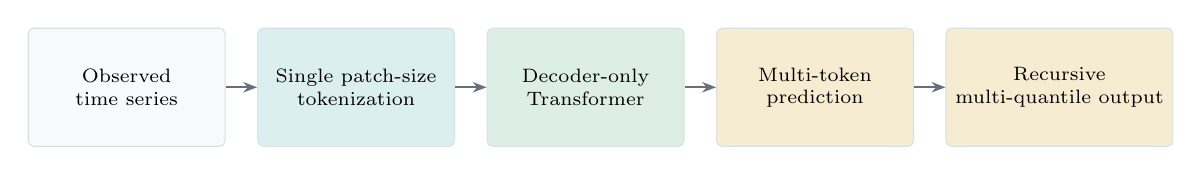
\begin{tikzpicture}[
      node distance=4mm,
      box/.style={draw=Line,rounded corners=2pt,align=center,
        minimum width=25mm,minimum height=15mm,font=\scriptsize},
      arrow/.style={-{Stealth[length=5pt]},thick,color=Muted}
    ]
      \node[box,fill=Paper] (series) {Observed\\time series};
      \node[box,fill=TealLight,right=of series] (patch) {Single patch-size\\tokenization};
      \node[box,fill=GreenLight,right=of patch] (decoder) {Decoder-only\\Transformer};
      \node[box,fill=GoldLight,right=of decoder] (multi) {Multi-token\\prediction};
      \node[box,fill=GoldLight,right=of multi] (quantile) {Recursive\\multi-quantile output};
      \draw[arrow] (series) -- (patch);
      \draw[arrow] (patch) -- (decoder);
      \draw[arrow] (decoder) -- (multi);
      \draw[arrow] (multi) -- (quantile);
    \end{tikzpicture}
  \end{center}

  \vspace{0.46cm}
  \begin{columns}[T,totalwidth=0.92\linewidth]
    \begin{column}{0.42\linewidth}
      \small
      \tagbox{TealLight}{\textbf{What changed from Moirai 1.0}}
      \vspace{0.14cm}
      \begin{itemize}
        \item Masked encoder $\rightarrow$ decoder-only
        \item Multiple patch sizes $\rightarrow$ one patch size
        \item Mixture distribution $\rightarrow$ direct quantiles
      \end{itemize}
    \end{column}
    \begin{column}{0.42\linewidth}
      \small
      \tagbox{GoldLight}{\textbf{Training objective}}
      \vspace{0.14cm}
      \begin{itemize}
        \item Quantile loss
        \item Multi-token prediction
        \item Recursive decoding over the requested horizon
        \item Pretrained on a corpus of 36M series
      \end{itemize}
    \end{column}
  \end{columns}

  \vfill
  {\tiny\color{Muted}Source: Liu et al., \emph{Moirai 2.0: When Less Is More for Time Series Forecasting}, 2025.}
\end{frame}

% ------------------------------------------------------------
\begin{frame}{Moirai 2.0 in this benchmark}
  \vspace{0.08cm}
  \begin{columns}[T,totalwidth=0.94\linewidth]
    \begin{column}{0.42\linewidth}
      \tagbox{GoldLight}{\textbf{Checkpoint and execution}}
      \vspace{0.20cm}
      \small
      \begin{itemize}
        \item Moirai 2.0-R Small
        \item Approximately 11.4M parameters
        \item CPU inference
        \item Maximum context: 512
        \item No dataset-specific fine-tuning
      \end{itemize}
    \end{column}
    \begin{column}{0.42\linewidth}
      \tagbox{GreenLight}{\textbf{Forecast interface}}
      \vspace{0.20cm}
      \small
      \begin{itemize}
        \item Direct quantiles 0.1 through 0.9
        \item Quantile 0.5 used as point forecast
        \item Deterministic benchmark call
        \item No separate predictive mean returned
      \end{itemize}
    \end{column}
  \end{columns}

  \vspace{0.42cm}
  \centering
  \begin{tabular}{L{0.23\linewidth} C{0.20\linewidth} C{0.20\linewidth} C{0.20\linewidth}}
    \toprule
    & \textbf{Chronos T5} & \textbf{TimesFM 2.5} & \textbf{Moirai 2.0} \\
    \midrule
    Backbone & Encoder--decoder & Decoder-only & Decoder-only \\
    Numerical interface & Discrete tokens & Continuous patches & Continuous patches \\
    Probabilistic output & Sample paths & Quantile head & Quantile head \\
    \bottomrule
  \end{tabular}

  \vfill
  {\tiny\color{Muted}Model: \texttt{Salesforce/moirai-2.0-R-small}, pinned revision \texttt{30f43ff}.}
\end{frame}

% ------------------------------------------------------------
\begin{frame}{Comparison models: five established forecasting references}
  \vspace{0.08cm}
  \scriptsize
  \renewcommand{\arraystretch}{1.30}
  \setlength{\tabcolsep}{4pt}
  \begin{center}
    \begin{tabular}{L{0.20\linewidth} L{0.34\linewidth} L{0.36\linewidth}}
      \toprule
      \textbf{Model} & \textbf{Forecast mechanism} & \textbf{Role in the comparison} \\
      \midrule
      ARIMA(2,1,2)
        & Fixed autoregressive, differencing, and moving-average structure
        & Compact classical model with Gaussian forecast intervals \\
      AutoARIMA
        & Searches configured ARIMA orders using an information criterion
        & Tests whether order selection improves on a fixed specification \\
      Prophet
        & Additive trend and seasonal components with predictive samples
        & Decomposition-based probabilistic baseline \\
      DeepAR
        & Autoregressive recurrent neural network with Student-$t$ output
        & Task-trained neural probabilistic baseline \\
      Seasonal Naive
        & Repeats the most recent seasonal pattern
        & Minimal seasonal reference with degenerate quantiles \\
      \bottomrule
    \end{tabular}
  \end{center}

  \vspace{0.40cm}
  \centering
  \tagbox{GrayLight}{\small Foundation models were used zero-shot; DeepAR and statistical models fit each forecast task.}
\end{frame}

\section{Datasets and Evaluation}

% ------------------------------------------------------------
\begin{frame}{Why these 12 datasets?}
  \vspace{0.08cm}
  \begin{columns}[T,totalwidth=0.95\linewidth]
    \begin{column}{0.43\linewidth}
      \tagbox{TealLight}{\textbf{Six Chronos / Monash benchmarks}}
      \vspace{0.18cm}
      \small
      \begin{itemize}
        \item M1 Yearly and M3 Quarterly
        \item M4 Hourly and NN5 Weekly
        \item Weather and Car Parts
      \end{itemize}
      \vspace{0.16cm}
      Public forecasting benchmarks provide established, heterogeneous
      reference tasks across frequencies and demand patterns.
    \end{column}
    \begin{column}{0.43\linewidth}
      \tagbox{GoldLight}{\textbf{Six external / official datasets}}
      \vspace{0.18cm}
      \small
      \begin{itemize}
        \item National Illness, Traffic, PSM
        \item Elexon electricity demand
        \item USGS streamflow
        \item BLS macroeconomic indicators
      \end{itemize}
      \vspace{0.16cm}
      These add health, mobility, industrial sensing, energy, hydrology,
      and macroeconomic domains.
    \end{column}
  \end{columns}

  \vspace{0.38cm}
  \centering
  \tagbox{GreenLight}{\small The portfolio tests transfer across domain, frequency, scale, seasonality, sparsity, and horizon.}
\end{frame}

% ------------------------------------------------------------
\begin{frame}{Dataset design: frequency, horizon, and seasonal scale}
  \vspace{-0.02cm}
  \scriptsize
  \renewcommand{\arraystretch}{1.20}
  \setlength{\tabcolsep}{3pt}
  \begin{columns}[T,totalwidth=0.97\linewidth]
    \begin{column}{0.48\linewidth}
      \begin{tabular}{L{0.42\linewidth} C{0.18\linewidth} C{0.16\linewidth} C{0.16\linewidth}}
        \toprule
        \textbf{Dataset} & \textbf{Freq.} & \textbf{Horizon} & \textbf{Lag} \\
        \midrule
        M1 Yearly & Yearly & 6 & 1 \\
        M4 Hourly & Hourly & 48 & 24 \\
        Weather & Daily & 30 & 7 \\
        M3 Quarterly & Quarterly & 8 & 4 \\
        Car Parts & Monthly & 12 & 12 \\
        NN5 Weekly & Weekly & 8 & 52 \\
        \bottomrule
      \end{tabular}
    \end{column}
    \begin{column}{0.48\linewidth}
      \begin{tabular}{L{0.42\linewidth} C{0.18\linewidth} C{0.16\linewidth} C{0.16\linewidth}}
        \toprule
        \textbf{Dataset} & \textbf{Freq.} & \textbf{Horizon} & \textbf{Lag} \\
        \midrule
        National Illness & Weekly & 24 & 52 \\
        Traffic & Hourly & 24 & 24 \\
        PSM & Hourly & 24 & 24 \\
        Elexon Demand & Daily & 30 & 7 \\
        USGS Streamflow & Daily & 30 & 365 \\
        BLS Macro & Monthly & 6 & 12 \\
        \bottomrule
      \end{tabular}
    \end{column}
  \end{columns}

  \vspace{0.44cm}
  \begin{columns}[T,totalwidth=0.93\linewidth]
    \begin{column}{0.28\linewidth}
      \tagbox{TealLight}{\small\textbf{Temporal breadth}}
      \vspace{0.13cm}
      \scriptsize Hourly through yearly sampling.
    \end{column}
    \begin{column}{0.28\linewidth}
      \tagbox{GoldLight}{\small\textbf{Pattern breadth}}
      \vspace{0.13cm}
      \scriptsize Smooth, seasonal, sparse, and volatile targets.
    \end{column}
    \begin{column}{0.28\linewidth}
      \tagbox{GreenLight}{\small\textbf{Operational breadth}}
      \vspace{0.13cm}
      \scriptsize Demand, health, transport, industry, water, and macro data.
    \end{column}
  \end{columns}
\end{frame}

% ------------------------------------------------------------
\begin{frame}{Five complementary evaluation metrics}
  \vspace{0.05cm}
  \scriptsize
  \renewcommand{\arraystretch}{1.28}
  \setlength{\tabcolsep}{4pt}
  \begin{center}
    \begin{tabular}{L{0.14\linewidth} L{0.35\linewidth} L{0.41\linewidth}}
      \toprule
      \textbf{Metric} & \textbf{Definition} & \textbf{What it emphasizes} \\
      \midrule
      MAE
        & Mean absolute median-forecast error
        & Typical absolute error in original target units \\
      RMSE
        & Square root of mean squared error
        & Larger misses receive greater weight \\
      sMAPE
        & Symmetric absolute percentage error
        & Scale-normalized relative point error \\
      MASE
        & MAE divided by in-sample seasonal-naive scale
        & Point error normalized by dataset seasonality \\
      WQL
        & Quantile loss normalized by total absolute target
        & Probabilistic accuracy across quantiles 0.1--0.9 \\
      \bottomrule
    \end{tabular}
  \end{center}

  \vspace{0.36cm}
  \begin{columns}[T,totalwidth=0.91\linewidth]
    \begin{column}{0.42\linewidth}
      \tagbox{GreenLight}{\textbf{All five: lower is better}}
      \vspace{0.14cm}
      \small Point metrics use the median forecast; WQL uses the full
      quantile forecast.
    \end{column}
    \begin{column}{0.42\linewidth}
      \tagbox{GoldLight}{\textbf{Dataset-level aggregation}}
      \vspace{0.14cm}
      \small Point metrics average task scores; official WQL combines
      loss and target-scale components.
    \end{column}
  \end{columns}
\end{frame}

% ------------------------------------------------------------
\begin{frame}{Common evaluation protocol}
  \vspace{0.08cm}
  \begin{columns}[T,totalwidth=0.95\linewidth]
    \begin{column}{0.43\linewidth}
      \tagbox{TealLight}{\textbf{Forecast tasks}}
      \vspace{0.18cm}
      \small
      \begin{itemize}
        \item Maximum context: 512 observations
        \item Dataset-specific horizon and seasonal lag
        \item Generally three rolling origins per series
        \item Two origins for Car Parts
        \item Representative series selection
      \end{itemize}
    \end{column}
    \begin{column}{0.43\linewidth}
      \tagbox{GoldLight}{\textbf{Forecast outputs}}
      \vspace{0.18cm}
      \small
      \begin{itemize}
        \item Median point forecast
        \item Quantiles 0.1 through 0.9
        \item Three repetitions for stochastic models
        \item Identical actual targets within each task
        \item Errors and durations retained
      \end{itemize}
    \end{column}
  \end{columns}

  \vspace{0.38cm}
  \centering
  \tagbox{GreenLight}{\small The result slides compare the same canonical 12-model view used to generate the final-clean plots.}
\end{frame}

\section{Performance Results}

% ------------------------------------------------------------
\begin{frame}{M1 Yearly: performance by metric}
  \vspace{-0.06cm}
  \begin{columns}[T,totalwidth=\linewidth]
    \begin{column}{0.49\linewidth}
      
\includegraphics[width=\linewidth,height=0.48\textheight,keepaspectratio]{chronos_m1_yearly/mase.png}
    \end{column}
    \begin{column}{0.49\linewidth}
      
\includegraphics[width=\linewidth,height=0.48\textheight,keepaspectratio]{chronos_m1_yearly/wql.png}
    \end{column}
  \end{columns}
  \vspace{0.06cm}
  \centering
  \scriptsize
  \setlength{\tabcolsep}{2pt}
  \begin{tabular}{C{0.19\linewidth} C{0.19\linewidth} C{0.19\linewidth} C{0.19\linewidth} C{0.19\linewidth}}
    \textbf{MAE} & \textbf{RMSE} & \textbf{sMAPE} & \textbf{MASE} & \textbf{WQL} \\[2pt]
    \winnerbox{PurpleLight}{DeepAR\\266,028} & \winnerbox{PurpleLight}{DeepAR\\289,227} & \winnerbox{CoralLight}{AutoARIMA\\0.2153} & \winnerbox{CoralLight}{AutoARIMA\\2.830} & \winnerbox{CoralLight}{ARIMA\\0.0827} \\
  \end{tabular}
  \vspace{0.05cm}
  {\tiny\color{Muted}Lower is better. Values are canonical dataset-level aggregates from the final clean runs.}
\end{frame}

% ------------------------------------------------------------
\begin{frame}{M4 Hourly: performance by metric}
  \vspace{-0.06cm}
  \begin{columns}[T,totalwidth=\linewidth]
    \begin{column}{0.49\linewidth}
      
\includegraphics[width=\linewidth,height=0.48\textheight,keepaspectratio]{chronos_m4_hourly/mase.png}
    \end{column}
    \begin{column}{0.49\linewidth}
      
\includegraphics[width=\linewidth,height=0.48\textheight,keepaspectratio]{chronos_m4_hourly/wql.png}
    \end{column}
  \end{columns}
  \vspace{0.06cm}
  \centering
  \scriptsize
  \setlength{\tabcolsep}{2pt}
  \begin{tabular}{C{0.19\linewidth} C{0.19\linewidth} C{0.19\linewidth} C{0.19\linewidth} C{0.19\linewidth}}
    \textbf{MAE} & \textbf{RMSE} & \textbf{sMAPE} & \textbf{MASE} & \textbf{WQL} \\[2pt]
    \winnerbox{TealLight}{Chronos Large\\122.249} & \winnerbox{TealLight}{Chronos Large\\161.491} & \winnerbox{TealLight}{Chronos Large\\0.0657} & \winnerbox{TealLight}{Chronos Large\\0.5240} & \winnerbox{TealLight}{Chronos Large\\0.0268} \\
  \end{tabular}
  \vspace{0.05cm}
  {\tiny\color{Muted}Lower is better. Values are canonical dataset-level aggregates from the final clean runs.}
\end{frame}

% ------------------------------------------------------------
\begin{frame}{Weather: performance by metric}
  \vspace{-0.06cm}
  \begin{columns}[T,totalwidth=\linewidth]
    \begin{column}{0.49\linewidth}
      
\includegraphics[width=\linewidth,height=0.48\textheight,keepaspectratio]{chronos_weather/mase.png}
    \end{column}
    \begin{column}{0.49\linewidth}
      
\includegraphics[width=\linewidth,height=0.48\textheight,keepaspectratio]{chronos_weather/wql.png}
    \end{column}
  \end{columns}
  \vspace{0.06cm}
  \centering
  \scriptsize
  \setlength{\tabcolsep}{2pt}
  \begin{tabular}{C{0.19\linewidth} C{0.19\linewidth} C{0.19\linewidth} C{0.19\linewidth} C{0.19\linewidth}}
    \textbf{MAE} & \textbf{RMSE} & \textbf{sMAPE} & \textbf{MASE} & \textbf{WQL} \\[2pt]
    \winnerbox{GoldLight}{Moirai\\1.365} & \winnerbox{GreenLight}{TimesFM\\2.869} & \winnerbox{GrayLight}{S. Naive\\0.7293} & \winnerbox{TealLight}{Chronos Large\\0.4275} & \winnerbox{GoldLight}{Moirai\\0.8569} \\
  \end{tabular}
  \vspace{0.05cm}
  {\tiny\color{Muted}Lower is better. Values are canonical dataset-level aggregates from the final clean runs.}
\end{frame}

% ------------------------------------------------------------
\begin{frame}{M3 Quarterly: performance by metric}
  \vspace{-0.06cm}
  \begin{columns}[T,totalwidth=\linewidth]
    \begin{column}{0.49\linewidth}
      
\includegraphics[width=\linewidth,height=0.48\textheight,keepaspectratio]{chronos_m3_quarterly/mase.png}
    \end{column}
    \begin{column}{0.49\linewidth}
      
\includegraphics[width=\linewidth,height=0.48\textheight,keepaspectratio]{chronos_m3_quarterly/wql.png}
    \end{column}
  \end{columns}
  \vspace{0.06cm}
  \centering
  \scriptsize
  \setlength{\tabcolsep}{2pt}
  \begin{tabular}{C{0.19\linewidth} C{0.19\linewidth} C{0.19\linewidth} C{0.19\linewidth} C{0.19\linewidth}}
    \textbf{MAE} & \textbf{RMSE} & \textbf{sMAPE} & \textbf{MASE} & \textbf{WQL} \\[2pt]
    \winnerbox{GreenLight}{TimesFM\\477.212} & \winnerbox{GreenLight}{TimesFM\\566.664} & \winnerbox{GreenLight}{TimesFM\\0.1083} & \winnerbox{GreenLight}{TimesFM\\1.145} & \winnerbox{GreenLight}{TimesFM\\0.0776} \\
  \end{tabular}
  \vspace{0.05cm}
  {\tiny\color{Muted}Lower is better. Values are canonical dataset-level aggregates from the final clean runs.}
\end{frame}

% ------------------------------------------------------------
\begin{frame}{Car Parts: performance by metric}
  \vspace{-0.06cm}
  \begin{columns}[T,totalwidth=\linewidth]
    \begin{column}{0.49\linewidth}
      
\includegraphics[width=\linewidth,height=0.48\textheight,keepaspectratio]{chronos_car_parts/mase.png}
    \end{column}
    \begin{column}{0.49\linewidth}
      
\includegraphics[width=\linewidth,height=0.48\textheight,keepaspectratio]{chronos_car_parts/wql.png}
    \end{column}
  \end{columns}
  \vspace{0.06cm}
  \centering
  \scriptsize
  \setlength{\tabcolsep}{2pt}
  \begin{tabular}{C{0.19\linewidth} C{0.19\linewidth} C{0.19\linewidth} C{0.19\linewidth} C{0.19\linewidth}}
    \textbf{MAE} & \textbf{RMSE} & \textbf{sMAPE} & \textbf{MASE} & \textbf{WQL} \\[2pt]
    \winnerbox{GoldLight}{Moirai\\0.3861} & \winnerbox{GoldLight}{Moirai\\0.6353} & \winnerbox{GrayLight}{S. Naive\\0.6735} & \winnerbox{GoldLight}{Moirai\\0.6904} & \winnerbox{GoldLight}{Moirai\\0.9325} \\
  \end{tabular}
  \vspace{0.05cm}
  {\tiny\color{Muted}Lower is better. Values are canonical dataset-level aggregates from the final clean runs.}
\end{frame}

% ------------------------------------------------------------
\begin{frame}{NN5 Weekly: performance by metric}
  \vspace{-0.06cm}
  \begin{columns}[T,totalwidth=\linewidth]
    \begin{column}{0.49\linewidth}
      
\includegraphics[width=\linewidth,height=0.48\textheight,keepaspectratio]{chronos_nn5_weekly/mase.png}
    \end{column}
    \begin{column}{0.49\linewidth}
      
\includegraphics[width=\linewidth,height=0.48\textheight,keepaspectratio]{chronos_nn5_weekly/wql.png}
    \end{column}
  \end{columns}
  \vspace{0.06cm}
  \centering
  \scriptsize
  \setlength{\tabcolsep}{2pt}
  \begin{tabular}{C{0.19\linewidth} C{0.19\linewidth} C{0.19\linewidth} C{0.19\linewidth} C{0.19\linewidth}}
    \textbf{MAE} & \textbf{RMSE} & \textbf{sMAPE} & \textbf{MASE} & \textbf{WQL} \\[2pt]
    \winnerbox{GreenLight}{TimesFM\\14.925} & \winnerbox{GreenLight}{TimesFM\\19.152} & \winnerbox{GreenLight}{TimesFM\\0.1097} & \winnerbox{GreenLight}{TimesFM\\0.8309} & \winnerbox{GreenLight}{TimesFM\\0.0840} \\
  \end{tabular}
  \vspace{0.05cm}
  {\tiny\color{Muted}Lower is better. Values are canonical dataset-level aggregates from the final clean runs.}
\end{frame}

% ------------------------------------------------------------
\begin{frame}{National Illness: performance by metric}
  \vspace{-0.06cm}
  \begin{columns}[T,totalwidth=\linewidth]
    \begin{column}{0.49\linewidth}
      
\includegraphics[width=\linewidth,height=0.48\textheight,keepaspectratio]{external_national_illness/mase.png}
    \end{column}
    \begin{column}{0.49\linewidth}
      
\includegraphics[width=\linewidth,height=0.48\textheight,keepaspectratio]{external_national_illness/wql.png}
    \end{column}
  \end{columns}
  \vspace{0.06cm}
  \centering
  \scriptsize
  \setlength{\tabcolsep}{2pt}
  \begin{tabular}{C{0.19\linewidth} C{0.19\linewidth} C{0.19\linewidth} C{0.19\linewidth} C{0.19\linewidth}}
    \textbf{MAE} & \textbf{RMSE} & \textbf{sMAPE} & \textbf{MASE} & \textbf{WQL} \\[2pt]
    \winnerbox{GreenLight}{TimesFM\\109,397} & \winnerbox{GreenLight}{TimesFM\\136,067} & \winnerbox{GreenLight}{TimesFM\\0.0897} & \winnerbox{GreenLight}{TimesFM\\1.326} & \winnerbox{GreenLight}{TimesFM\\0.0688} \\
  \end{tabular}
  \vspace{0.05cm}
  {\tiny\color{Muted}Lower is better. Values are canonical dataset-level aggregates from the final clean runs.}
\end{frame}

% ------------------------------------------------------------
\begin{frame}{Traffic: performance by metric}
  \vspace{-0.06cm}
  \begin{columns}[T,totalwidth=\linewidth]
    \begin{column}{0.49\linewidth}
      
\includegraphics[width=\linewidth,height=0.48\textheight,keepaspectratio]{external_traffic/mase.png}
    \end{column}
    \begin{column}{0.49\linewidth}
      
\includegraphics[width=\linewidth,height=0.48\textheight,keepaspectratio]{external_traffic/wql.png}
    \end{column}
  \end{columns}
  \vspace{0.06cm}
  \centering
  \scriptsize
  \setlength{\tabcolsep}{2pt}
  \begin{tabular}{C{0.19\linewidth} C{0.19\linewidth} C{0.19\linewidth} C{0.19\linewidth} C{0.19\linewidth}}
    \textbf{MAE} & \textbf{RMSE} & \textbf{sMAPE} & \textbf{MASE} & \textbf{WQL} \\[2pt]
    \winnerbox{GoldLight}{Moirai\\0.00547} & \winnerbox{GoldLight}{Moirai\\0.00673} & \winnerbox{TealLight}{Chronos Large\\0.1698} & \winnerbox{TealLight}{Chronos Large\\0.4746} & \winnerbox{GoldLight}{Moirai\\0.1436} \\
  \end{tabular}
  \vspace{0.05cm}
  {\tiny\color{Muted}Lower is better. Values are canonical dataset-level aggregates from the final clean runs.}
\end{frame}

% ------------------------------------------------------------
\begin{frame}{PSM: performance by metric}
  \vspace{-0.06cm}
  \begin{columns}[T,totalwidth=\linewidth]
    \begin{column}{0.49\linewidth}
      
\includegraphics[width=\linewidth,height=0.48\textheight,keepaspectratio]{external_psm/mase.png}
    \end{column}
    \begin{column}{0.49\linewidth}
      
\includegraphics[width=\linewidth,height=0.48\textheight,keepaspectratio]{external_psm/wql.png}
    \end{column}
  \end{columns}
  \vspace{0.06cm}
  \centering
  \scriptsize
  \setlength{\tabcolsep}{2pt}
  \begin{tabular}{C{0.19\linewidth} C{0.19\linewidth} C{0.19\linewidth} C{0.19\linewidth} C{0.19\linewidth}}
    \textbf{MAE} & \textbf{RMSE} & \textbf{sMAPE} & \textbf{MASE} & \textbf{WQL} \\[2pt]
    \winnerbox{TealLight}{Chronos Small\\0.0145} & \winnerbox{TealLight}{Chronos Small\\0.0195} & \winnerbox{TealLight}{Chronos Small\\0.0432} & \winnerbox{TealLight}{Chronos Small\\0.5101} & \winnerbox{TealLight}{Chronos Small\\0.0270} \\
  \end{tabular}
  \vspace{0.05cm}
  {\tiny\color{Muted}Lower is better. Values are canonical dataset-level aggregates from the final clean runs.}
\end{frame}

% ------------------------------------------------------------
\begin{frame}{Elexon Electricity Demand: performance by metric}
  \vspace{-0.06cm}
  \begin{columns}[T,totalwidth=\linewidth]
    \begin{column}{0.49\linewidth}
      
\includegraphics[width=\linewidth,height=0.48\textheight,keepaspectratio]{official_elexon_demand/mase.png}
    \end{column}
    \begin{column}{0.49\linewidth}
      
\includegraphics[width=\linewidth,height=0.48\textheight,keepaspectratio]{official_elexon_demand/wql.png}
    \end{column}
  \end{columns}
  \vspace{0.06cm}
  \centering
  \scriptsize
  \setlength{\tabcolsep}{2pt}
  \begin{tabular}{C{0.19\linewidth} C{0.19\linewidth} C{0.19\linewidth} C{0.19\linewidth} C{0.19\linewidth}}
    \textbf{MAE} & \textbf{RMSE} & \textbf{sMAPE} & \textbf{MASE} & \textbf{WQL} \\[2pt]
    \winnerbox{TealLight}{Chronos Large\\25,175.2} & \winnerbox{TealLight}{Chronos Large\\30,732.0} & \winnerbox{TealLight}{Chronos Large\\0.0473} & \winnerbox{TealLight}{Chronos Large\\0.5810} & \winnerbox{TealLight}{Chronos Large\\0.0362} \\
  \end{tabular}
  \vspace{0.05cm}
  {\tiny\color{Muted}Lower is better. Values are canonical dataset-level aggregates from the final clean runs.}
\end{frame}

% ------------------------------------------------------------
\begin{frame}{USGS Streamflow: performance by metric}
  \vspace{-0.06cm}
  \begin{columns}[T,totalwidth=\linewidth]
    \begin{column}{0.49\linewidth}
      
\includegraphics[width=\linewidth,height=0.48\textheight,keepaspectratio]{official_usgs_streamflow/mase.png}
    \end{column}
    \begin{column}{0.49\linewidth}
      
\includegraphics[width=\linewidth,height=0.48\textheight,keepaspectratio]{official_usgs_streamflow/wql.png}
    \end{column}
  \end{columns}
  \vspace{0.06cm}
  \centering
  \scriptsize
  \setlength{\tabcolsep}{2pt}
  \begin{tabular}{C{0.19\linewidth} C{0.19\linewidth} C{0.19\linewidth} C{0.19\linewidth} C{0.19\linewidth}}
    \textbf{MAE} & \textbf{RMSE} & \textbf{sMAPE} & \textbf{MASE} & \textbf{WQL} \\[2pt]
    \winnerbox{GreenLight}{TimesFM\\1,482.4} & \winnerbox{GreenLight}{TimesFM\\2,288.6} & \winnerbox{GoldLight}{Moirai\\0.3173} & \winnerbox{GoldLight}{Moirai\\1.088} & \winnerbox{GreenLight}{TimesFM\\0.2601} \\
  \end{tabular}
  \vspace{0.05cm}
  {\tiny\color{Muted}Lower is better. Values are canonical dataset-level aggregates from the final clean runs.}
\end{frame}

% ------------------------------------------------------------
\begin{frame}{BLS Macroeconomic Indicators: performance by metric}
  \vspace{-0.06cm}
  \begin{columns}[T,totalwidth=\linewidth]
    \begin{column}{0.49\linewidth}
      
\includegraphics[width=\linewidth,height=0.48\textheight,keepaspectratio]{official_bls_macro/mase.png}
    \end{column}
    \begin{column}{0.49\linewidth}
      
\includegraphics[width=\linewidth,height=0.48\textheight,keepaspectratio]{official_bls_macro/wql.png}
    \end{column}
  \end{columns}
  \vspace{0.06cm}
  \centering
  \scriptsize
  \setlength{\tabcolsep}{2pt}
  \begin{tabular}{C{0.19\linewidth} C{0.19\linewidth} C{0.19\linewidth} C{0.19\linewidth} C{0.19\linewidth}}
    \textbf{MAE} & \textbf{RMSE} & \textbf{sMAPE} & \textbf{MASE} & \textbf{WQL} \\[2pt]
    \winnerbox{GreenLight}{TimesFM\\66.455} & \winnerbox{GreenLight}{TimesFM\\77.532} & \winnerbox{CoralLight}{ARIMA\\0.0125} & \winnerbox{CoralLight}{ARIMA\\0.1580} & \winnerbox{GreenLight}{TimesFM\\0.00108} \\
  \end{tabular}
  \vspace{0.05cm}
  {\tiny\color{Muted}Lower is better. Values are canonical dataset-level aggregates from the final clean runs.}
\end{frame}

% ------------------------------------------------------------
\begin{frame}{Winner matrix: model with the lowest aggregate metric}
  \vspace{-0.10cm}
  \centering
  \tiny
  \renewcommand{\arraystretch}{1.28}
  \setlength{\tabcolsep}{2.5pt}
  \begin{tabular}{L{0.27\linewidth} C{0.13\linewidth} C{0.13\linewidth} C{0.13\linewidth} C{0.13\linewidth} C{0.13\linewidth}}
    \toprule
    \textbf{Dataset} & \textbf{MAE} & \textbf{RMSE} & \textbf{sMAPE} & \textbf{MASE} & \textbf{WQL} \\
    \midrule
    M1 Yearly & \cellcolor{PurpleLight}\textbf{DeepAR} & \cellcolor{PurpleLight}\textbf{DeepAR} & \cellcolor{CoralLight}\textbf{AutoARIMA} & \cellcolor{CoralLight}\textbf{AutoARIMA} & \cellcolor{CoralLight}\textbf{ARIMA} \\
    M4 Hourly & \cellcolor{TealLight}\textbf{Chronos Large} & \cellcolor{TealLight}\textbf{Chronos Large} & \cellcolor{TealLight}\textbf{Chronos Large} & \cellcolor{TealLight}\textbf{Chronos Large} & \cellcolor{TealLight}\textbf{Chronos Large} \\
    Weather & \cellcolor{GoldLight}\textbf{Moirai} & \cellcolor{GreenLight}\textbf{TimesFM} & \cellcolor{GrayLight}\textbf{S. Naive} & \cellcolor{TealLight}\textbf{Chronos Large} & \cellcolor{GoldLight}\textbf{Moirai} \\
    M3 Quarterly & \cellcolor{GreenLight}\textbf{TimesFM} & \cellcolor{GreenLight}\textbf{TimesFM} & \cellcolor{GreenLight}\textbf{TimesFM} & \cellcolor{GreenLight}\textbf{TimesFM} & \cellcolor{GreenLight}\textbf{TimesFM} \\
    Car Parts & \cellcolor{GoldLight}\textbf{Moirai} & \cellcolor{GoldLight}\textbf{Moirai} & \cellcolor{GrayLight}\textbf{S. Naive} & \cellcolor{GoldLight}\textbf{Moirai} & \cellcolor{GoldLight}\textbf{Moirai} \\
    NN5 Weekly & \cellcolor{GreenLight}\textbf{TimesFM} & \cellcolor{GreenLight}\textbf{TimesFM} & \cellcolor{GreenLight}\textbf{TimesFM} & \cellcolor{GreenLight}\textbf{TimesFM} & \cellcolor{GreenLight}\textbf{TimesFM} \\
    National Illness & \cellcolor{GreenLight}\textbf{TimesFM} & \cellcolor{GreenLight}\textbf{TimesFM} & \cellcolor{GreenLight}\textbf{TimesFM} & \cellcolor{GreenLight}\textbf{TimesFM} & \cellcolor{GreenLight}\textbf{TimesFM} \\
    Traffic & \cellcolor{GoldLight}\textbf{Moirai} & \cellcolor{GoldLight}\textbf{Moirai} & \cellcolor{TealLight}\textbf{Chronos Large} & \cellcolor{TealLight}\textbf{Chronos Large} & \cellcolor{GoldLight}\textbf{Moirai} \\
    PSM & \cellcolor{TealLight}\textbf{Chronos Small} & \cellcolor{TealLight}\textbf{Chronos Small} & \cellcolor{TealLight}\textbf{Chronos Small} & \cellcolor{TealLight}\textbf{Chronos Small} & \cellcolor{TealLight}\textbf{Chronos Small} \\
    Elexon Electricity Demand & \cellcolor{TealLight}\textbf{Chronos Large} & \cellcolor{TealLight}\textbf{Chronos Large} & \cellcolor{TealLight}\textbf{Chronos Large} & \cellcolor{TealLight}\textbf{Chronos Large} & \cellcolor{TealLight}\textbf{Chronos Large} \\
    USGS Streamflow & \cellcolor{GreenLight}\textbf{TimesFM} & \cellcolor{GreenLight}\textbf{TimesFM} & \cellcolor{GoldLight}\textbf{Moirai} & \cellcolor{GoldLight}\textbf{Moirai} & \cellcolor{GreenLight}\textbf{TimesFM} \\
    BLS Macroeconomic Indicators & \cellcolor{GreenLight}\textbf{TimesFM} & \cellcolor{GreenLight}\textbf{TimesFM} & \cellcolor{CoralLight}\textbf{ARIMA} & \cellcolor{CoralLight}\textbf{ARIMA} & \cellcolor{GreenLight}\textbf{TimesFM} \\
    \bottomrule
  \end{tabular}
  \vspace{0.16cm}
  {\scriptsize\color{Muted}Each cell reports the minimum among the 12 evaluated models for that dataset and metric.}
\end{frame}

% ------------------------------------------------------------
\begin{frame}{How often each model wins a dataset--metric cell}
  \vspace{0.08cm}
  \begin{columns}[T,totalwidth=0.94\linewidth]
    \begin{column}{0.48\linewidth}
      \small
      \renewcommand{\arraystretch}{1.30}
      \setlength{\tabcolsep}{5pt}
      \begin{tabular}{L{0.66\linewidth} C{0.20\linewidth}}
        \toprule
        \textbf{Model} & \textbf{Wins} \\
        \midrule
        \cellcolor{GreenLight}TimesFM 2.5 & \textbf{22} \\
        \cellcolor{TealLight}Chronos Large & \textbf{13} \\
        \cellcolor{GoldLight}Moirai 2.0 & \textbf{11} \\
        \cellcolor{TealLight}Chronos Small & \textbf{5} \\
        \cellcolor{CoralLight}ARIMA(2,1,2) & \textbf{3} \\
        \cellcolor{PurpleLight}DeepAR & \textbf{2} \\
        \cellcolor{CoralLight}AutoARIMA & \textbf{2} \\
        \cellcolor{GrayLight}Seasonal Naive & \textbf{2} \\
        \bottomrule
      \end{tabular}
    \end{column}
    \begin{column}{0.40\linewidth}
      \small
      \tagbox{GreenLight}{\textbf{60 winner cells}}
      \vspace{0.22cm}
      \begin{itemize}
        \item 12 datasets $\times$ 5 core metrics.
        \item A win is the lowest aggregate metric value.
        \item Counts summarize breadth, not statistical significance.
        \item Metrics are correlated, so five wins on one dataset are not five independent experiments.
      \end{itemize}
    \end{column}
  \end{columns}
\end{frame}


% ------------------------------------------------------------
\begin{frame}{Interpretation boundaries}
  \vspace{0.08cm}
  \begin{columns}[T,totalwidth=0.94\linewidth]
    \begin{column}{0.43\linewidth}
      \tagbox{GoldLight}{\textbf{Metric boundaries}}
      \vspace{0.18cm}
      \small
      \begin{itemize}
        \item MAE and RMSE are scale-dependent.
        \item sMAPE is unstable around zero.
        \item Official WQL weights tasks by target magnitude.
        \item The five metrics are correlated.
      \end{itemize}
    \end{column}
    \begin{column}{0.43\linewidth}
      \tagbox{CoralLight}{\textbf{Experimental boundaries}}
      \vspace{0.18cm}
      \small
      \begin{itemize}
        \item Winner cells are descriptive aggregate minima.
        \item No statistical significance test was applied.
        \item Eligible series counts differ by dataset.
        \item Some Moirai trajectories contain quantile crossings.
      \end{itemize}
    \end{column}
  \end{columns}

  \vspace{0.42cm}
  \centering
  \widebox{GrayLight}{\small Use the winner matrix as a benchmark summary, not as a universal ranking independent of dataset and objective.}
\end{frame}

% ------------------------------------------------------------
\begin{frame}{Conclusions}
  \vspace{0.08cm}
  \begin{columns}[T,totalwidth=0.95\linewidth]
    \begin{column}{0.44\linewidth}
      \tagbox{GreenLight}{\textbf{Foundation-model breadth}}
      \vspace{0.18cm}
      \small
      \begin{itemize}
        \item TimesFM records 22 of 60 winner cells.
        \item Chronos Large records 13; Moirai records 11.
        \item Chronos Small sweeps all five PSM metrics.
        \item Foundation models collectively win 51 of 60 cells.
      \end{itemize}
    \end{column}
    \begin{column}{0.44\linewidth}
      \tagbox{GoldLight}{\textbf{Dataset dependence remains}}
      \vspace{0.18cm}
      \small
      \begin{itemize}
        \item TimesFM sweeps M3, NN5, and National Illness.
        \item Chronos Large sweeps M4 and Elexon.
        \item Moirai leads most Car Parts and Traffic metrics.
        \item Classical and trained neural baselines still win selected cells.
      \end{itemize}
    \end{column}
  \end{columns}

  \vspace{0.40cm}
  \begin{center}
    \begin{minipage}{0.87\linewidth}
      \large\raggedright
      \key{Main result:} pretrained foundation models dominate the aggregate
      winner count, but the best choice still changes with dataset, metric,
      and checkpoint scale.
    \end{minipage}
  \end{center}
\end{frame}

% ------------------------------------------------------------
\begin{frame}{Architecture references}
  \vspace{0.08cm}
  \scriptsize
  \begin{itemize}
    \item Ansari et al. (2024), \emph{Chronos: Learning the Language of Time Series},
      Transactions on Machine Learning Research. \texttt{arXiv:2403.07815}
    \item Amazon Science, official \texttt{chronos-t5-*} model cards and
      \texttt{amazon-science/chronos-forecasting} implementation.
    \item Das et al. (2024), \emph{A Decoder-Only Foundation Model for
      Time-Series Forecasting}, ICML. \texttt{arXiv:2310.10688}
    \item Google Research, official TimesFM 2.5 PyTorch implementation and
      \texttt{google/timesfm-2.5-200m-pytorch} model release.
    \item Liu et al. (2025), \emph{Moirai 2.0: When Less Is More for Time
      Series Forecasting}. \texttt{arXiv:2511.11698}
    \item Salesforce AI Research, \texttt{uni2ts} implementation and
      \texttt{Salesforce/moirai-2.0-R-small} model release.
  \end{itemize}

  \vspace{0.35cm}
  \tagbox{GrayLight}{\small Performance figures and tables are generated from \texttt{pmds/results/final\_clean\_results}.}
\end{frame}

\appendix
\section{Appendix}
% ------------------------------------------------------------
\begin{frame}[plain]
  \vspace{1.25cm}
  {\color{Teal}\rule{1.25cm}{3pt}}
  \vspace{0.45cm}
  {\fontsize{28}{33}\selectfont\bfseries Appendix\par}
  \vspace{0.30cm}
  {\Large\color{Muted}Complete metric and forecast-trajectory plots\par}
\end{frame}

% ------------------------------------------------------------
\begin{frame}{M1 Yearly --- MAE}
  \centering
  
\includegraphics[width=\linewidth,height=0.79\textheight,keepaspectratio]{chronos_m1_yearly/mae.png}
\end{frame}

% ------------------------------------------------------------
\begin{frame}{M1 Yearly --- RMSE}
  \centering
  
\includegraphics[width=\linewidth,height=0.79\textheight,keepaspectratio]{chronos_m1_yearly/rmse.png}
\end{frame}

% ------------------------------------------------------------
\begin{frame}{M1 Yearly --- sMAPE}
  \centering
  
\includegraphics[width=\linewidth,height=0.79\textheight,keepaspectratio]{chronos_m1_yearly/smape.png}
\end{frame}

% ------------------------------------------------------------
\begin{frame}{M1 Yearly --- MASE}
  \centering
  
\includegraphics[width=\linewidth,height=0.79\textheight,keepaspectratio]{chronos_m1_yearly/mase.png}
\end{frame}

% ------------------------------------------------------------
\begin{frame}{M1 Yearly --- WQL}
  \centering
  
\includegraphics[width=\linewidth,height=0.79\textheight,keepaspectratio]{chronos_m1_yearly/wql.png}
\end{frame}

% ------------------------------------------------------------
\begin{frame}{M1 Yearly --- Macro WQL}
  \centering
  
\includegraphics[width=\linewidth,height=0.79\textheight,keepaspectratio]{chronos_m1_yearly/wql_macro.png}
\end{frame}

% ------------------------------------------------------------
\begin{frame}{M1 Yearly --- Within-metric ranks}
  \centering
  
\includegraphics[width=\linewidth,height=0.79\textheight,keepaspectratio]{chronos_m1_yearly/all_metrics_normalized.png}
\end{frame}

% ------------------------------------------------------------
\begin{frame}{M1 Yearly --- Rank heatmap}
  \centering
  
\includegraphics[width=\linewidth,height=0.79\textheight,keepaspectratio]{chronos_m1_yearly/all_metrics_dot_comparison.png}
\end{frame}

% ------------------------------------------------------------
\begin{frame}{M4 Hourly --- MAE}
  \centering
  
\includegraphics[width=\linewidth,height=0.79\textheight,keepaspectratio]{chronos_m4_hourly/mae.png}
\end{frame}

% ------------------------------------------------------------
\begin{frame}{M4 Hourly --- RMSE}
  \centering
  
\includegraphics[width=\linewidth,height=0.79\textheight,keepaspectratio]{chronos_m4_hourly/rmse.png}
\end{frame}

% ------------------------------------------------------------
\begin{frame}{M4 Hourly --- sMAPE}
  \centering
  
\includegraphics[width=\linewidth,height=0.79\textheight,keepaspectratio]{chronos_m4_hourly/smape.png}
\end{frame}

% ------------------------------------------------------------
\begin{frame}{M4 Hourly --- MASE}
  \centering
  
\includegraphics[width=\linewidth,height=0.79\textheight,keepaspectratio]{chronos_m4_hourly/mase.png}
\end{frame}

% ------------------------------------------------------------
\begin{frame}{M4 Hourly --- WQL}
  \centering
  
\includegraphics[width=\linewidth,height=0.79\textheight,keepaspectratio]{chronos_m4_hourly/wql.png}
\end{frame}

% ------------------------------------------------------------
\begin{frame}{M4 Hourly --- Macro WQL}
  \centering
  
\includegraphics[width=\linewidth,height=0.79\textheight,keepaspectratio]{chronos_m4_hourly/wql_macro.png}
\end{frame}

% ------------------------------------------------------------
\begin{frame}{M4 Hourly --- Within-metric ranks}
  \centering
  
\includegraphics[width=\linewidth,height=0.79\textheight,keepaspectratio]{chronos_m4_hourly/all_metrics_normalized.png}
\end{frame}

% ------------------------------------------------------------
\begin{frame}{M4 Hourly --- Rank heatmap}
  \centering
  
\includegraphics[width=\linewidth,height=0.79\textheight,keepaspectratio]{chronos_m4_hourly/all_metrics_dot_comparison.png}
\end{frame}

% ------------------------------------------------------------
\begin{frame}{Weather --- MAE}
  \centering
  
\includegraphics[width=\linewidth,height=0.79\textheight,keepaspectratio]{chronos_weather/mae.png}
\end{frame}

% ------------------------------------------------------------
\begin{frame}{Weather --- RMSE}
  \centering
  
\includegraphics[width=\linewidth,height=0.79\textheight,keepaspectratio]{chronos_weather/rmse.png}
\end{frame}

% ------------------------------------------------------------
\begin{frame}{Weather --- sMAPE}
  \centering
  
\includegraphics[width=\linewidth,height=0.79\textheight,keepaspectratio]{chronos_weather/smape.png}
\end{frame}

% ------------------------------------------------------------
\begin{frame}{Weather --- MASE}
  \centering
  
\includegraphics[width=\linewidth,height=0.79\textheight,keepaspectratio]{chronos_weather/mase.png}
\end{frame}

% ------------------------------------------------------------
\begin{frame}{Weather --- WQL}
  \centering
  
\includegraphics[width=\linewidth,height=0.79\textheight,keepaspectratio]{chronos_weather/wql.png}
\end{frame}

% ------------------------------------------------------------
\begin{frame}{Weather --- Macro WQL}
  \centering
  
\includegraphics[width=\linewidth,height=0.79\textheight,keepaspectratio]{chronos_weather/wql_macro.png}
\end{frame}

% ------------------------------------------------------------
\begin{frame}{Weather --- Rain occurrence error}
  \centering
  
\includegraphics[width=\linewidth,height=0.79\textheight,keepaspectratio]{chronos_weather/rain_occurrence_error.png}
\end{frame}

% ------------------------------------------------------------
\begin{frame}{Weather --- Positive-value MAE}
  \centering
  
\includegraphics[width=\linewidth,height=0.79\textheight,keepaspectratio]{chronos_weather/positive_mae.png}
\end{frame}

% ------------------------------------------------------------
\begin{frame}{Weather --- Within-metric ranks}
  \centering
  
\includegraphics[width=\linewidth,height=0.79\textheight,keepaspectratio]{chronos_weather/all_metrics_normalized.png}
\end{frame}

% ------------------------------------------------------------
\begin{frame}{Weather --- Rank heatmap}
  \centering
  
\includegraphics[width=\linewidth,height=0.79\textheight,keepaspectratio]{chronos_weather/all_metrics_dot_comparison.png}
\end{frame}

% ------------------------------------------------------------
\begin{frame}{M3 Quarterly --- MAE}
  \centering
  
\includegraphics[width=\linewidth,height=0.79\textheight,keepaspectratio]{chronos_m3_quarterly/mae.png}
\end{frame}

% ------------------------------------------------------------
\begin{frame}{M3 Quarterly --- RMSE}
  \centering
  
\includegraphics[width=\linewidth,height=0.79\textheight,keepaspectratio]{chronos_m3_quarterly/rmse.png}
\end{frame}

% ------------------------------------------------------------
\begin{frame}{M3 Quarterly --- sMAPE}
  \centering
  
\includegraphics[width=\linewidth,height=0.79\textheight,keepaspectratio]{chronos_m3_quarterly/smape.png}
\end{frame}

% ------------------------------------------------------------
\begin{frame}{M3 Quarterly --- MASE}
  \centering
  
\includegraphics[width=\linewidth,height=0.79\textheight,keepaspectratio]{chronos_m3_quarterly/mase.png}
\end{frame}

% ------------------------------------------------------------
\begin{frame}{M3 Quarterly --- WQL}
  \centering
  
\includegraphics[width=\linewidth,height=0.79\textheight,keepaspectratio]{chronos_m3_quarterly/wql.png}
\end{frame}

% ------------------------------------------------------------
\begin{frame}{M3 Quarterly --- Macro WQL}
  \centering
  
\includegraphics[width=\linewidth,height=0.79\textheight,keepaspectratio]{chronos_m3_quarterly/wql_macro.png}
\end{frame}

% ------------------------------------------------------------
\begin{frame}{M3 Quarterly --- Within-metric ranks}
  \centering
  
\includegraphics[width=\linewidth,height=0.79\textheight,keepaspectratio]{chronos_m3_quarterly/all_metrics_normalized.png}
\end{frame}

% ------------------------------------------------------------
\begin{frame}{M3 Quarterly --- Rank heatmap}
  \centering
  
\includegraphics[width=\linewidth,height=0.79\textheight,keepaspectratio]{chronos_m3_quarterly/all_metrics_dot_comparison.png}
\end{frame}

% ------------------------------------------------------------
\begin{frame}{Car Parts --- MAE}
  \centering
  
\includegraphics[width=\linewidth,height=0.79\textheight,keepaspectratio]{chronos_car_parts/mae.png}
\end{frame}

% ------------------------------------------------------------
\begin{frame}{Car Parts --- RMSE}
  \centering
  
\includegraphics[width=\linewidth,height=0.79\textheight,keepaspectratio]{chronos_car_parts/rmse.png}
\end{frame}

% ------------------------------------------------------------
\begin{frame}{Car Parts --- sMAPE}
  \centering
  
\includegraphics[width=\linewidth,height=0.79\textheight,keepaspectratio]{chronos_car_parts/smape.png}
\end{frame}

% ------------------------------------------------------------
\begin{frame}{Car Parts --- MASE}
  \centering
  
\includegraphics[width=\linewidth,height=0.79\textheight,keepaspectratio]{chronos_car_parts/mase.png}
\end{frame}

% ------------------------------------------------------------
\begin{frame}{Car Parts --- WQL}
  \centering
  
\includegraphics[width=\linewidth,height=0.79\textheight,keepaspectratio]{chronos_car_parts/wql.png}
\end{frame}

% ------------------------------------------------------------
\begin{frame}{Car Parts --- Macro WQL}
  \centering
  
\includegraphics[width=\linewidth,height=0.79\textheight,keepaspectratio]{chronos_car_parts/wql_macro.png}
\end{frame}

% ------------------------------------------------------------
\begin{frame}{Car Parts --- Rain occurrence error}
  \centering
  
\includegraphics[width=\linewidth,height=0.79\textheight,keepaspectratio]{chronos_car_parts/rain_occurrence_error.png}
\end{frame}

% ------------------------------------------------------------
\begin{frame}{Car Parts --- Positive-value MAE}
  \centering
  
\includegraphics[width=\linewidth,height=0.79\textheight,keepaspectratio]{chronos_car_parts/positive_mae.png}
\end{frame}

% ------------------------------------------------------------
\begin{frame}{Car Parts --- Within-metric ranks}
  \centering
  
\includegraphics[width=\linewidth,height=0.79\textheight,keepaspectratio]{chronos_car_parts/all_metrics_normalized.png}
\end{frame}

% ------------------------------------------------------------
\begin{frame}{Car Parts --- Rank heatmap}
  \centering
  
\includegraphics[width=\linewidth,height=0.79\textheight,keepaspectratio]{chronos_car_parts/all_metrics_dot_comparison.png}
\end{frame}

% ------------------------------------------------------------
\begin{frame}{NN5 Weekly --- MAE}
  \centering
  
\includegraphics[width=\linewidth,height=0.79\textheight,keepaspectratio]{chronos_nn5_weekly/mae.png}
\end{frame}

% ------------------------------------------------------------
\begin{frame}{NN5 Weekly --- RMSE}
  \centering
  
\includegraphics[width=\linewidth,height=0.79\textheight,keepaspectratio]{chronos_nn5_weekly/rmse.png}
\end{frame}

% ------------------------------------------------------------
\begin{frame}{NN5 Weekly --- sMAPE}
  \centering
  
\includegraphics[width=\linewidth,height=0.79\textheight,keepaspectratio]{chronos_nn5_weekly/smape.png}
\end{frame}

% ------------------------------------------------------------
\begin{frame}{NN5 Weekly --- MASE}
  \centering
  
\includegraphics[width=\linewidth,height=0.79\textheight,keepaspectratio]{chronos_nn5_weekly/mase.png}
\end{frame}

% ------------------------------------------------------------
\begin{frame}{NN5 Weekly --- WQL}
  \centering
  
\includegraphics[width=\linewidth,height=0.79\textheight,keepaspectratio]{chronos_nn5_weekly/wql.png}
\end{frame}

% ------------------------------------------------------------
\begin{frame}{NN5 Weekly --- Macro WQL}
  \centering
  
\includegraphics[width=\linewidth,height=0.79\textheight,keepaspectratio]{chronos_nn5_weekly/wql_macro.png}
\end{frame}

% ------------------------------------------------------------
\begin{frame}{NN5 Weekly --- Within-metric ranks}
  \centering
  
\includegraphics[width=\linewidth,height=0.79\textheight,keepaspectratio]{chronos_nn5_weekly/all_metrics_normalized.png}
\end{frame}

% ------------------------------------------------------------
\begin{frame}{NN5 Weekly --- Rank heatmap}
  \centering
  
\includegraphics[width=\linewidth,height=0.79\textheight,keepaspectratio]{chronos_nn5_weekly/all_metrics_dot_comparison.png}
\end{frame}

% ------------------------------------------------------------
\begin{frame}{National Illness --- MAE}
  \centering
  
\includegraphics[width=\linewidth,height=0.79\textheight,keepaspectratio]{external_national_illness/mae.png}
\end{frame}

% ------------------------------------------------------------
\begin{frame}{National Illness --- RMSE}
  \centering
  
\includegraphics[width=\linewidth,height=0.79\textheight,keepaspectratio]{external_national_illness/rmse.png}
\end{frame}

% ------------------------------------------------------------
\begin{frame}{National Illness --- sMAPE}
  \centering
  
\includegraphics[width=\linewidth,height=0.79\textheight,keepaspectratio]{external_national_illness/smape.png}
\end{frame}

% ------------------------------------------------------------
\begin{frame}{National Illness --- MASE}
  \centering
  
\includegraphics[width=\linewidth,height=0.79\textheight,keepaspectratio]{external_national_illness/mase.png}
\end{frame}

% ------------------------------------------------------------
\begin{frame}{National Illness --- WQL}
  \centering
  
\includegraphics[width=\linewidth,height=0.79\textheight,keepaspectratio]{external_national_illness/wql.png}
\end{frame}

% ------------------------------------------------------------
\begin{frame}{National Illness --- Macro WQL}
  \centering
  
\includegraphics[width=\linewidth,height=0.79\textheight,keepaspectratio]{external_national_illness/wql_macro.png}
\end{frame}

% ------------------------------------------------------------
\begin{frame}{National Illness --- Within-metric ranks}
  \centering
  
\includegraphics[width=\linewidth,height=0.79\textheight,keepaspectratio]{external_national_illness/all_metrics_normalized.png}
\end{frame}

% ------------------------------------------------------------
\begin{frame}{National Illness --- Rank heatmap}
  \centering
  
\includegraphics[width=\linewidth,height=0.79\textheight,keepaspectratio]{external_national_illness/all_metrics_dot_comparison.png}
\end{frame}

% ------------------------------------------------------------
\begin{frame}{Traffic --- MAE}
  \centering
  
\includegraphics[width=\linewidth,height=0.79\textheight,keepaspectratio]{external_traffic/mae.png}
\end{frame}

% ------------------------------------------------------------
\begin{frame}{Traffic --- RMSE}
  \centering
  
\includegraphics[width=\linewidth,height=0.79\textheight,keepaspectratio]{external_traffic/rmse.png}
\end{frame}

% ------------------------------------------------------------
\begin{frame}{Traffic --- sMAPE}
  \centering
  
\includegraphics[width=\linewidth,height=0.79\textheight,keepaspectratio]{external_traffic/smape.png}
\end{frame}

% ------------------------------------------------------------
\begin{frame}{Traffic --- MASE}
  \centering
  
\includegraphics[width=\linewidth,height=0.79\textheight,keepaspectratio]{external_traffic/mase.png}
\end{frame}

% ------------------------------------------------------------
\begin{frame}{Traffic --- WQL}
  \centering
  
\includegraphics[width=\linewidth,height=0.79\textheight,keepaspectratio]{external_traffic/wql.png}
\end{frame}

% ------------------------------------------------------------
\begin{frame}{Traffic --- Macro WQL}
  \centering
  
\includegraphics[width=\linewidth,height=0.79\textheight,keepaspectratio]{external_traffic/wql_macro.png}
\end{frame}

% ------------------------------------------------------------
\begin{frame}{Traffic --- Within-metric ranks}
  \centering
  
\includegraphics[width=\linewidth,height=0.79\textheight,keepaspectratio]{external_traffic/all_metrics_normalized.png}
\end{frame}

% ------------------------------------------------------------
\begin{frame}{Traffic --- Rank heatmap}
  \centering
  
\includegraphics[width=\linewidth,height=0.79\textheight,keepaspectratio]{external_traffic/all_metrics_dot_comparison.png}
\end{frame}

% ------------------------------------------------------------
\begin{frame}{PSM --- MAE}
  \centering
  
\includegraphics[width=\linewidth,height=0.79\textheight,keepaspectratio]{external_psm/mae.png}
\end{frame}

% ------------------------------------------------------------
\begin{frame}{PSM --- RMSE}
  \centering
  
\includegraphics[width=\linewidth,height=0.79\textheight,keepaspectratio]{external_psm/rmse.png}
\end{frame}

% ------------------------------------------------------------
\begin{frame}{PSM --- sMAPE}
  \centering
  
\includegraphics[width=\linewidth,height=0.79\textheight,keepaspectratio]{external_psm/smape.png}
\end{frame}

% ------------------------------------------------------------
\begin{frame}{PSM --- MASE}
  \centering
  
\includegraphics[width=\linewidth,height=0.79\textheight,keepaspectratio]{external_psm/mase.png}
\end{frame}

% ------------------------------------------------------------
\begin{frame}{PSM --- WQL}
  \centering
  
\includegraphics[width=\linewidth,height=0.79\textheight,keepaspectratio]{external_psm/wql.png}
\end{frame}

% ------------------------------------------------------------
\begin{frame}{PSM --- Macro WQL}
  \centering
  
\includegraphics[width=\linewidth,height=0.79\textheight,keepaspectratio]{external_psm/wql_macro.png}
\end{frame}

% ------------------------------------------------------------
\begin{frame}{PSM --- Within-metric ranks}
  \centering
  
\includegraphics[width=\linewidth,height=0.79\textheight,keepaspectratio]{external_psm/all_metrics_normalized.png}
\end{frame}

% ------------------------------------------------------------
\begin{frame}{PSM --- Rank heatmap}
  \centering
  
\includegraphics[width=\linewidth,height=0.79\textheight,keepaspectratio]{external_psm/all_metrics_dot_comparison.png}
\end{frame}

% ------------------------------------------------------------
\begin{frame}{Elexon Demand --- MAE}
  \centering
  
\includegraphics[width=\linewidth,height=0.79\textheight,keepaspectratio]{official_elexon_demand/mae.png}
\end{frame}

% ------------------------------------------------------------
\begin{frame}{Elexon Demand --- RMSE}
  \centering
  
\includegraphics[width=\linewidth,height=0.79\textheight,keepaspectratio]{official_elexon_demand/rmse.png}
\end{frame}

% ------------------------------------------------------------
\begin{frame}{Elexon Demand --- sMAPE}
  \centering
  
\includegraphics[width=\linewidth,height=0.79\textheight,keepaspectratio]{official_elexon_demand/smape.png}
\end{frame}

% ------------------------------------------------------------
\begin{frame}{Elexon Demand --- MASE}
  \centering
  
\includegraphics[width=\linewidth,height=0.79\textheight,keepaspectratio]{official_elexon_demand/mase.png}
\end{frame}

% ------------------------------------------------------------
\begin{frame}{Elexon Demand --- WQL}
  \centering
  
\includegraphics[width=\linewidth,height=0.79\textheight,keepaspectratio]{official_elexon_demand/wql.png}
\end{frame}

% ------------------------------------------------------------
\begin{frame}{Elexon Demand --- Macro WQL}
  \centering
  
\includegraphics[width=\linewidth,height=0.79\textheight,keepaspectratio]{official_elexon_demand/wql_macro.png}
\end{frame}

% ------------------------------------------------------------
\begin{frame}{Elexon Demand --- Within-metric ranks}
  \centering
  
\includegraphics[width=\linewidth,height=0.79\textheight,keepaspectratio]{official_elexon_demand/all_metrics_normalized.png}
\end{frame}

% ------------------------------------------------------------
\begin{frame}{Elexon Demand --- Rank heatmap}
  \centering
  
\includegraphics[width=\linewidth,height=0.79\textheight,keepaspectratio]{official_elexon_demand/all_metrics_dot_comparison.png}
\end{frame}

% ------------------------------------------------------------
\begin{frame}{USGS Streamflow --- MAE}
  \centering
  
\includegraphics[width=\linewidth,height=0.79\textheight,keepaspectratio]{official_usgs_streamflow/mae.png}
\end{frame}

% ------------------------------------------------------------
\begin{frame}{USGS Streamflow --- RMSE}
  \centering
  
\includegraphics[width=\linewidth,height=0.79\textheight,keepaspectratio]{official_usgs_streamflow/rmse.png}
\end{frame}

% ------------------------------------------------------------
\begin{frame}{USGS Streamflow --- sMAPE}
  \centering
  
\includegraphics[width=\linewidth,height=0.79\textheight,keepaspectratio]{official_usgs_streamflow/smape.png}
\end{frame}

% ------------------------------------------------------------
\begin{frame}{USGS Streamflow --- MASE}
  \centering
  
\includegraphics[width=\linewidth,height=0.79\textheight,keepaspectratio]{official_usgs_streamflow/mase.png}
\end{frame}

% ------------------------------------------------------------
\begin{frame}{USGS Streamflow --- WQL}
  \centering
  
\includegraphics[width=\linewidth,height=0.79\textheight,keepaspectratio]{official_usgs_streamflow/wql.png}
\end{frame}

% ------------------------------------------------------------
\begin{frame}{USGS Streamflow --- Macro WQL}
  \centering
  
\includegraphics[width=\linewidth,height=0.79\textheight,keepaspectratio]{official_usgs_streamflow/wql_macro.png}
\end{frame}

% ------------------------------------------------------------
\begin{frame}{USGS Streamflow --- Within-metric ranks}
  \centering
  
\includegraphics[width=\linewidth,height=0.79\textheight,keepaspectratio]{official_usgs_streamflow/all_metrics_normalized.png}
\end{frame}

% ------------------------------------------------------------
\begin{frame}{USGS Streamflow --- Rank heatmap}
  \centering
  
\includegraphics[width=\linewidth,height=0.79\textheight,keepaspectratio]{official_usgs_streamflow/all_metrics_dot_comparison.png}
\end{frame}

% ------------------------------------------------------------
\begin{frame}{BLS Macro Indicators --- MAE}
  \centering
  
\includegraphics[width=\linewidth,height=0.79\textheight,keepaspectratio]{official_bls_macro/mae.png}
\end{frame}

% ------------------------------------------------------------
\begin{frame}{BLS Macro Indicators --- RMSE}
  \centering
  
\includegraphics[width=\linewidth,height=0.79\textheight,keepaspectratio]{official_bls_macro/rmse.png}
\end{frame}

% ------------------------------------------------------------
\begin{frame}{BLS Macro Indicators --- sMAPE}
  \centering
  
\includegraphics[width=\linewidth,height=0.79\textheight,keepaspectratio]{official_bls_macro/smape.png}
\end{frame}

% ------------------------------------------------------------
\begin{frame}{BLS Macro Indicators --- MASE}
  \centering
  
\includegraphics[width=\linewidth,height=0.79\textheight,keepaspectratio]{official_bls_macro/mase.png}
\end{frame}

% ------------------------------------------------------------
\begin{frame}{BLS Macro Indicators --- WQL}
  \centering
  
\includegraphics[width=\linewidth,height=0.79\textheight,keepaspectratio]{official_bls_macro/wql.png}
\end{frame}

% ------------------------------------------------------------
\begin{frame}{BLS Macro Indicators --- Macro WQL}
  \centering
  
\includegraphics[width=\linewidth,height=0.79\textheight,keepaspectratio]{official_bls_macro/wql_macro.png}
\end{frame}

% ------------------------------------------------------------
\begin{frame}{BLS Macro Indicators --- Within-metric ranks}
  \centering
  
\includegraphics[width=\linewidth,height=0.79\textheight,keepaspectratio]{official_bls_macro/all_metrics_normalized.png}
\end{frame}

% ------------------------------------------------------------
\begin{frame}{BLS Macro Indicators --- Rank heatmap}
  \centering
  
\includegraphics[width=\linewidth,height=0.79\textheight,keepaspectratio]{official_bls_macro/all_metrics_dot_comparison.png}
\end{frame}

% ------------------------------------------------------------
\begin{frame}{M1 Yearly --- forecast vs. actual --- Chronos Tiny}
  \centering
  
\includegraphics[width=\linewidth,height=0.79\textheight,keepaspectratio]{chronos_m1_yearly/forecast_vs_actual/chronos_t5_tiny.png}
\end{frame}

% ------------------------------------------------------------
\begin{frame}{M1 Yearly --- forecast vs. actual --- TimesFM 2.5}
  \centering
  
\includegraphics[width=\linewidth,height=0.79\textheight,keepaspectratio]{chronos_m1_yearly/forecast_vs_actual/timesfm_2_5_200m.png}
\end{frame}

% ------------------------------------------------------------
\begin{frame}{M1 Yearly --- forecast vs. actual --- Moirai 2.0}
  \centering
  
\includegraphics[width=\linewidth,height=0.79\textheight,keepaspectratio]{chronos_m1_yearly/forecast_vs_actual/moirai_2_0_small.png}
\end{frame}

% ------------------------------------------------------------
\begin{frame}{M1 Yearly --- forecast vs. actual --- Seasonal Naive}
  \centering
  
\includegraphics[width=\linewidth,height=0.79\textheight,keepaspectratio]{chronos_m1_yearly/forecast_vs_actual/seasonal_naive.png}
\end{frame}

% ------------------------------------------------------------
\begin{frame}{M1 Yearly --- forecast vs. actual --- ARIMA(2,1,2)}
  \centering
  
\includegraphics[width=\linewidth,height=0.79\textheight,keepaspectratio]{chronos_m1_yearly/forecast_vs_actual/arima_2_1_2.png}
\end{frame}

% ------------------------------------------------------------
\begin{frame}{M1 Yearly --- forecast vs. actual --- AutoARIMA}
  \centering
  
\includegraphics[width=\linewidth,height=0.79\textheight,keepaspectratio]{chronos_m1_yearly/forecast_vs_actual/auto_arima.png}
\end{frame}

% ------------------------------------------------------------
\begin{frame}{M1 Yearly --- forecast vs. actual --- Prophet}
  \centering
  
\includegraphics[width=\linewidth,height=0.79\textheight,keepaspectratio]{chronos_m1_yearly/forecast_vs_actual/prophet.png}
\end{frame}

% ------------------------------------------------------------
\begin{frame}{M1 Yearly --- forecast vs. actual --- DeepAR}
  \centering
  
\includegraphics[width=\linewidth,height=0.79\textheight,keepaspectratio]{chronos_m1_yearly/forecast_vs_actual/deepar.png}
\end{frame}

% ------------------------------------------------------------
\begin{frame}{M1 Yearly --- forecast vs. actual --- Chronos Mini}
  \centering
  
\includegraphics[width=\linewidth,height=0.79\textheight,keepaspectratio]{chronos_m1_yearly/forecast_vs_actual/chronos_t5_mini.png}
\end{frame}

% ------------------------------------------------------------
\begin{frame}{M1 Yearly --- forecast vs. actual --- Chronos Small}
  \centering
  
\includegraphics[width=\linewidth,height=0.79\textheight,keepaspectratio]{chronos_m1_yearly/forecast_vs_actual/chronos_t5_small.png}
\end{frame}

% ------------------------------------------------------------
\begin{frame}{M1 Yearly --- forecast vs. actual --- Chronos Base}
  \centering
  
\includegraphics[width=\linewidth,height=0.79\textheight,keepaspectratio]{chronos_m1_yearly/forecast_vs_actual/chronos_t5_base.png}
\end{frame}

% ------------------------------------------------------------
\begin{frame}{M1 Yearly --- forecast vs. actual --- Chronos Large}
  \centering
  
\includegraphics[width=\linewidth,height=0.79\textheight,keepaspectratio]{chronos_m1_yearly/forecast_vs_actual/chronos_t5_large.png}
\end{frame}

% ------------------------------------------------------------
\begin{frame}{M4 Hourly --- forecast vs. actual --- Chronos Tiny}
  \centering
  
\includegraphics[width=\linewidth,height=0.79\textheight,keepaspectratio]{chronos_m4_hourly/forecast_vs_actual/chronos_t5_tiny.png}
\end{frame}

% ------------------------------------------------------------
\begin{frame}{M4 Hourly --- forecast vs. actual --- TimesFM 2.5}
  \centering
  
\includegraphics[width=\linewidth,height=0.79\textheight,keepaspectratio]{chronos_m4_hourly/forecast_vs_actual/timesfm_2_5_200m.png}
\end{frame}

% ------------------------------------------------------------
\begin{frame}{M4 Hourly --- forecast vs. actual --- Moirai 2.0}
  \centering
  
\includegraphics[width=\linewidth,height=0.79\textheight,keepaspectratio]{chronos_m4_hourly/forecast_vs_actual/moirai_2_0_small.png}
\end{frame}

% ------------------------------------------------------------
\begin{frame}{M4 Hourly --- forecast vs. actual --- Seasonal Naive}
  \centering
  
\includegraphics[width=\linewidth,height=0.79\textheight,keepaspectratio]{chronos_m4_hourly/forecast_vs_actual/seasonal_naive.png}
\end{frame}

% ------------------------------------------------------------
\begin{frame}{M4 Hourly --- forecast vs. actual --- ARIMA(2,1,2)}
  \centering
  
\includegraphics[width=\linewidth,height=0.79\textheight,keepaspectratio]{chronos_m4_hourly/forecast_vs_actual/arima_2_1_2.png}
\end{frame}

% ------------------------------------------------------------
\begin{frame}{M4 Hourly --- forecast vs. actual --- AutoARIMA}
  \centering
  
\includegraphics[width=\linewidth,height=0.79\textheight,keepaspectratio]{chronos_m4_hourly/forecast_vs_actual/auto_arima.png}
\end{frame}

% ------------------------------------------------------------
\begin{frame}{M4 Hourly --- forecast vs. actual --- Prophet}
  \centering
  
\includegraphics[width=\linewidth,height=0.79\textheight,keepaspectratio]{chronos_m4_hourly/forecast_vs_actual/prophet.png}
\end{frame}

% ------------------------------------------------------------
\begin{frame}{M4 Hourly --- forecast vs. actual --- DeepAR}
  \centering
  
\includegraphics[width=\linewidth,height=0.79\textheight,keepaspectratio]{chronos_m4_hourly/forecast_vs_actual/deepar.png}
\end{frame}

% ------------------------------------------------------------
\begin{frame}{M4 Hourly --- forecast vs. actual --- Chronos Mini}
  \centering
  
\includegraphics[width=\linewidth,height=0.79\textheight,keepaspectratio]{chronos_m4_hourly/forecast_vs_actual/chronos_t5_mini.png}
\end{frame}

% ------------------------------------------------------------
\begin{frame}{M4 Hourly --- forecast vs. actual --- Chronos Small}
  \centering
  
\includegraphics[width=\linewidth,height=0.79\textheight,keepaspectratio]{chronos_m4_hourly/forecast_vs_actual/chronos_t5_small.png}
\end{frame}

% ------------------------------------------------------------
\begin{frame}{M4 Hourly --- forecast vs. actual --- Chronos Base}
  \centering
  
\includegraphics[width=\linewidth,height=0.79\textheight,keepaspectratio]{chronos_m4_hourly/forecast_vs_actual/chronos_t5_base.png}
\end{frame}

% ------------------------------------------------------------
\begin{frame}{M4 Hourly --- forecast vs. actual --- Chronos Large}
  \centering
  
\includegraphics[width=\linewidth,height=0.79\textheight,keepaspectratio]{chronos_m4_hourly/forecast_vs_actual/chronos_t5_large.png}
\end{frame}

% ------------------------------------------------------------
\begin{frame}{Weather --- forecast vs. actual --- Chronos Tiny}
  \centering
  
\includegraphics[width=\linewidth,height=0.79\textheight,keepaspectratio]{chronos_weather/forecast_vs_actual/chronos_t5_tiny.png}
\end{frame}

% ------------------------------------------------------------
\begin{frame}{Weather --- forecast vs. actual --- TimesFM 2.5}
  \centering
  
\includegraphics[width=\linewidth,height=0.79\textheight,keepaspectratio]{chronos_weather/forecast_vs_actual/timesfm_2_5_200m.png}
\end{frame}

% ------------------------------------------------------------
\begin{frame}{Weather --- forecast vs. actual --- Moirai 2.0}
  \centering
  
\includegraphics[width=\linewidth,height=0.79\textheight,keepaspectratio]{chronos_weather/forecast_vs_actual/moirai_2_0_small.png}
\end{frame}

% ------------------------------------------------------------
\begin{frame}{Weather --- forecast vs. actual --- Seasonal Naive}
  \centering
  
\includegraphics[width=\linewidth,height=0.79\textheight,keepaspectratio]{chronos_weather/forecast_vs_actual/seasonal_naive.png}
\end{frame}

% ------------------------------------------------------------
\begin{frame}{Weather --- forecast vs. actual --- ARIMA(2,1,2)}
  \centering
  
\includegraphics[width=\linewidth,height=0.79\textheight,keepaspectratio]{chronos_weather/forecast_vs_actual/arima_2_1_2.png}
\end{frame}

% ------------------------------------------------------------
\begin{frame}{Weather --- forecast vs. actual --- AutoARIMA}
  \centering
  
\includegraphics[width=\linewidth,height=0.79\textheight,keepaspectratio]{chronos_weather/forecast_vs_actual/auto_arima.png}
\end{frame}

% ------------------------------------------------------------
\begin{frame}{Weather --- forecast vs. actual --- Prophet}
  \centering
  
\includegraphics[width=\linewidth,height=0.79\textheight,keepaspectratio]{chronos_weather/forecast_vs_actual/prophet.png}
\end{frame}

% ------------------------------------------------------------
\begin{frame}{Weather --- forecast vs. actual --- DeepAR}
  \centering
  
\includegraphics[width=\linewidth,height=0.79\textheight,keepaspectratio]{chronos_weather/forecast_vs_actual/deepar.png}
\end{frame}

% ------------------------------------------------------------
\begin{frame}{Weather --- forecast vs. actual --- Chronos Mini}
  \centering
  
\includegraphics[width=\linewidth,height=0.79\textheight,keepaspectratio]{chronos_weather/forecast_vs_actual/chronos_t5_mini.png}
\end{frame}

% ------------------------------------------------------------
\begin{frame}{Weather --- forecast vs. actual --- Chronos Small}
  \centering
  
\includegraphics[width=\linewidth,height=0.79\textheight,keepaspectratio]{chronos_weather/forecast_vs_actual/chronos_t5_small.png}
\end{frame}

% ------------------------------------------------------------
\begin{frame}{Weather --- forecast vs. actual --- Chronos Base}
  \centering
  
\includegraphics[width=\linewidth,height=0.79\textheight,keepaspectratio]{chronos_weather/forecast_vs_actual/chronos_t5_base.png}
\end{frame}

% ------------------------------------------------------------
\begin{frame}{Weather --- forecast vs. actual --- Chronos Large}
  \centering
  
\includegraphics[width=\linewidth,height=0.79\textheight,keepaspectratio]{chronos_weather/forecast_vs_actual/chronos_t5_large.png}
\end{frame}

% ------------------------------------------------------------
\begin{frame}{M3 Quarterly --- forecast vs. actual --- Chronos Tiny}
  \centering
  
\includegraphics[width=\linewidth,height=0.79\textheight,keepaspectratio]{chronos_m3_quarterly/forecast_vs_actual/chronos_t5_tiny.png}
\end{frame}

% ------------------------------------------------------------
\begin{frame}{M3 Quarterly --- forecast vs. actual --- TimesFM 2.5}
  \centering
  
\includegraphics[width=\linewidth,height=0.79\textheight,keepaspectratio]{chronos_m3_quarterly/forecast_vs_actual/timesfm_2_5_200m.png}
\end{frame}

% ------------------------------------------------------------
\begin{frame}{M3 Quarterly --- forecast vs. actual --- Moirai 2.0}
  \centering
  
\includegraphics[width=\linewidth,height=0.79\textheight,keepaspectratio]{chronos_m3_quarterly/forecast_vs_actual/moirai_2_0_small.png}
\end{frame}

% ------------------------------------------------------------
\begin{frame}{M3 Quarterly --- forecast vs. actual --- Seasonal Naive}
  \centering
  
\includegraphics[width=\linewidth,height=0.79\textheight,keepaspectratio]{chronos_m3_quarterly/forecast_vs_actual/seasonal_naive.png}
\end{frame}

% ------------------------------------------------------------
\begin{frame}{M3 Quarterly --- forecast vs. actual --- ARIMA(2,1,2)}
  \centering
  
\includegraphics[width=\linewidth,height=0.79\textheight,keepaspectratio]{chronos_m3_quarterly/forecast_vs_actual/arima_2_1_2.png}
\end{frame}

% ------------------------------------------------------------
\begin{frame}{M3 Quarterly --- forecast vs. actual --- AutoARIMA}
  \centering
  
\includegraphics[width=\linewidth,height=0.79\textheight,keepaspectratio]{chronos_m3_quarterly/forecast_vs_actual/auto_arima.png}
\end{frame}

% ------------------------------------------------------------
\begin{frame}{M3 Quarterly --- forecast vs. actual --- Prophet}
  \centering
  
\includegraphics[width=\linewidth,height=0.79\textheight,keepaspectratio]{chronos_m3_quarterly/forecast_vs_actual/prophet.png}
\end{frame}

% ------------------------------------------------------------
\begin{frame}{M3 Quarterly --- forecast vs. actual --- DeepAR}
  \centering
  
\includegraphics[width=\linewidth,height=0.79\textheight,keepaspectratio]{chronos_m3_quarterly/forecast_vs_actual/deepar.png}
\end{frame}

% ------------------------------------------------------------
\begin{frame}{M3 Quarterly --- forecast vs. actual --- Chronos Mini}
  \centering
  
\includegraphics[width=\linewidth,height=0.79\textheight,keepaspectratio]{chronos_m3_quarterly/forecast_vs_actual/chronos_t5_mini.png}
\end{frame}

% ------------------------------------------------------------
\begin{frame}{M3 Quarterly --- forecast vs. actual --- Chronos Small}
  \centering
  
\includegraphics[width=\linewidth,height=0.79\textheight,keepaspectratio]{chronos_m3_quarterly/forecast_vs_actual/chronos_t5_small.png}
\end{frame}

% ------------------------------------------------------------
\begin{frame}{M3 Quarterly --- forecast vs. actual --- Chronos Base}
  \centering
  
\includegraphics[width=\linewidth,height=0.79\textheight,keepaspectratio]{chronos_m3_quarterly/forecast_vs_actual/chronos_t5_base.png}
\end{frame}

% ------------------------------------------------------------
\begin{frame}{M3 Quarterly --- forecast vs. actual --- Chronos Large}
  \centering
  
\includegraphics[width=\linewidth,height=0.79\textheight,keepaspectratio]{chronos_m3_quarterly/forecast_vs_actual/chronos_t5_large.png}
\end{frame}

% ------------------------------------------------------------
\begin{frame}{Car Parts --- forecast vs. actual --- Chronos Tiny}
  \centering
  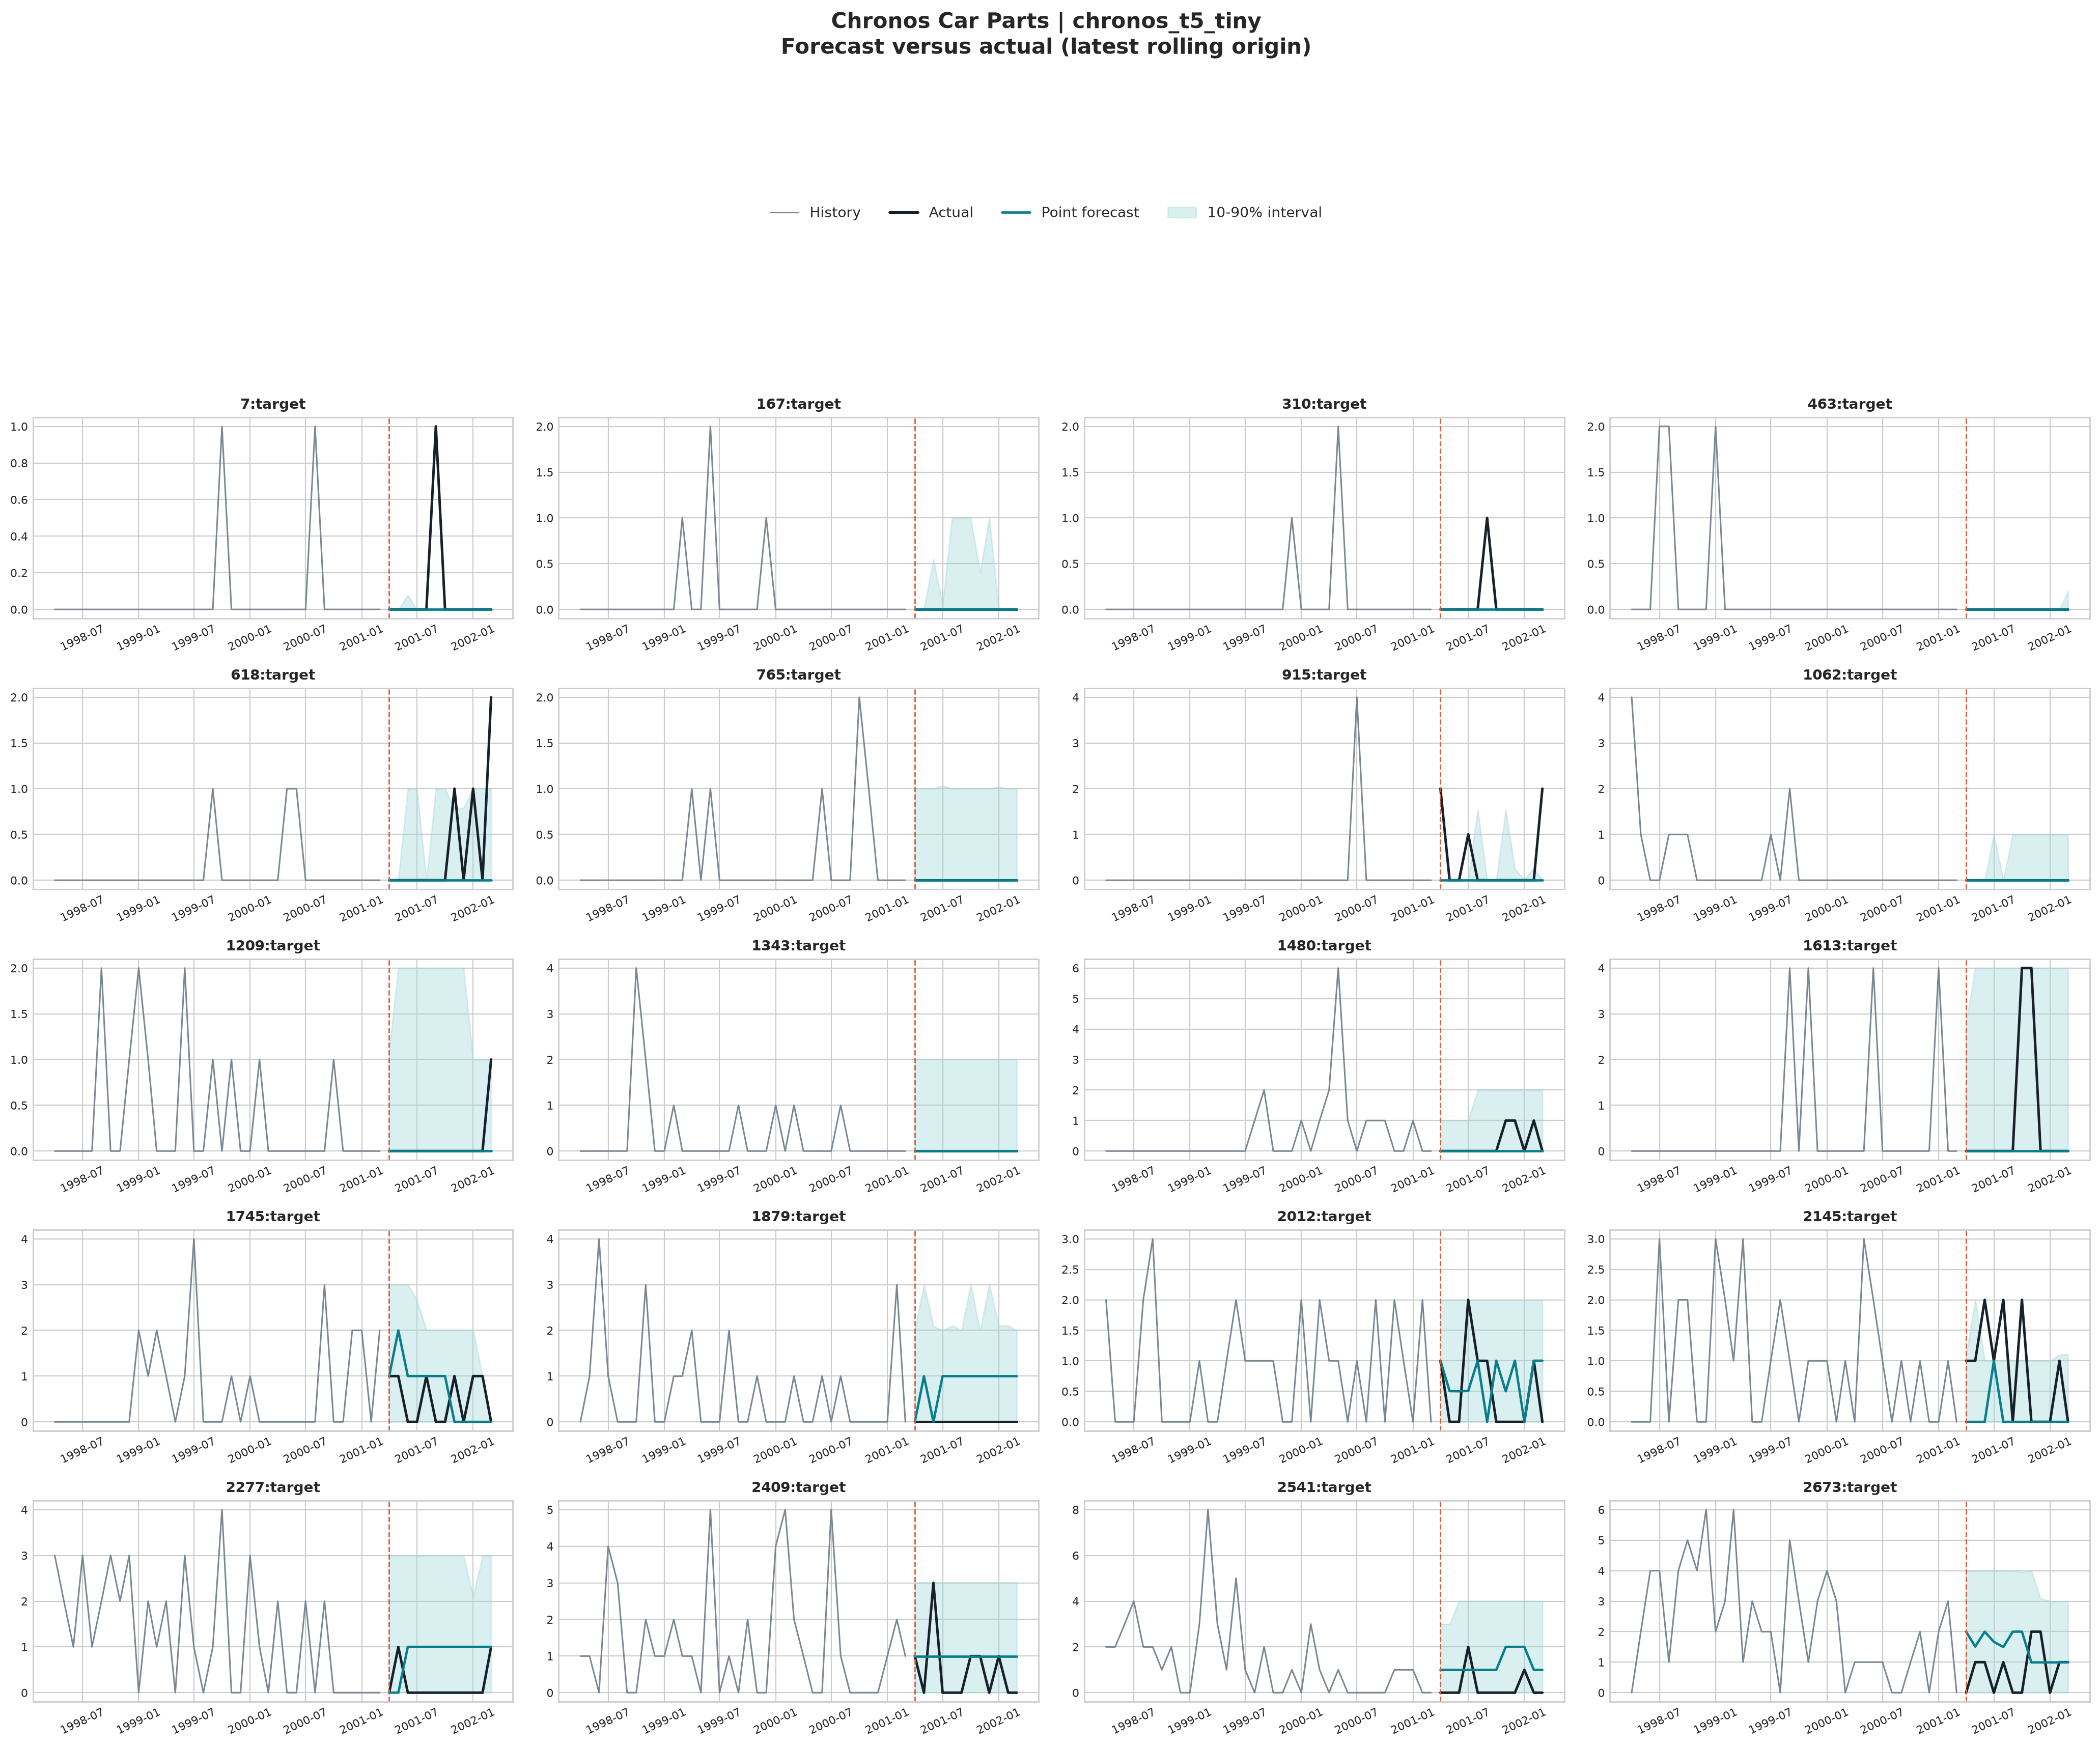
\includegraphics[width=\linewidth,height=0.79\textheight,keepaspectratio]{chronos_car_parts/forecast_vs_actual/chronos_t5_tiny.png}
\end{frame}

% ------------------------------------------------------------
\begin{frame}{Car Parts --- forecast vs. actual --- TimesFM 2.5}
  \centering
  
\includegraphics[width=\linewidth,height=0.79\textheight,keepaspectratio]{chronos_car_parts/forecast_vs_actual/timesfm_2_5_200m.png}
\end{frame}

% ------------------------------------------------------------
\begin{frame}{Car Parts --- forecast vs. actual --- Moirai 2.0}
  \centering
  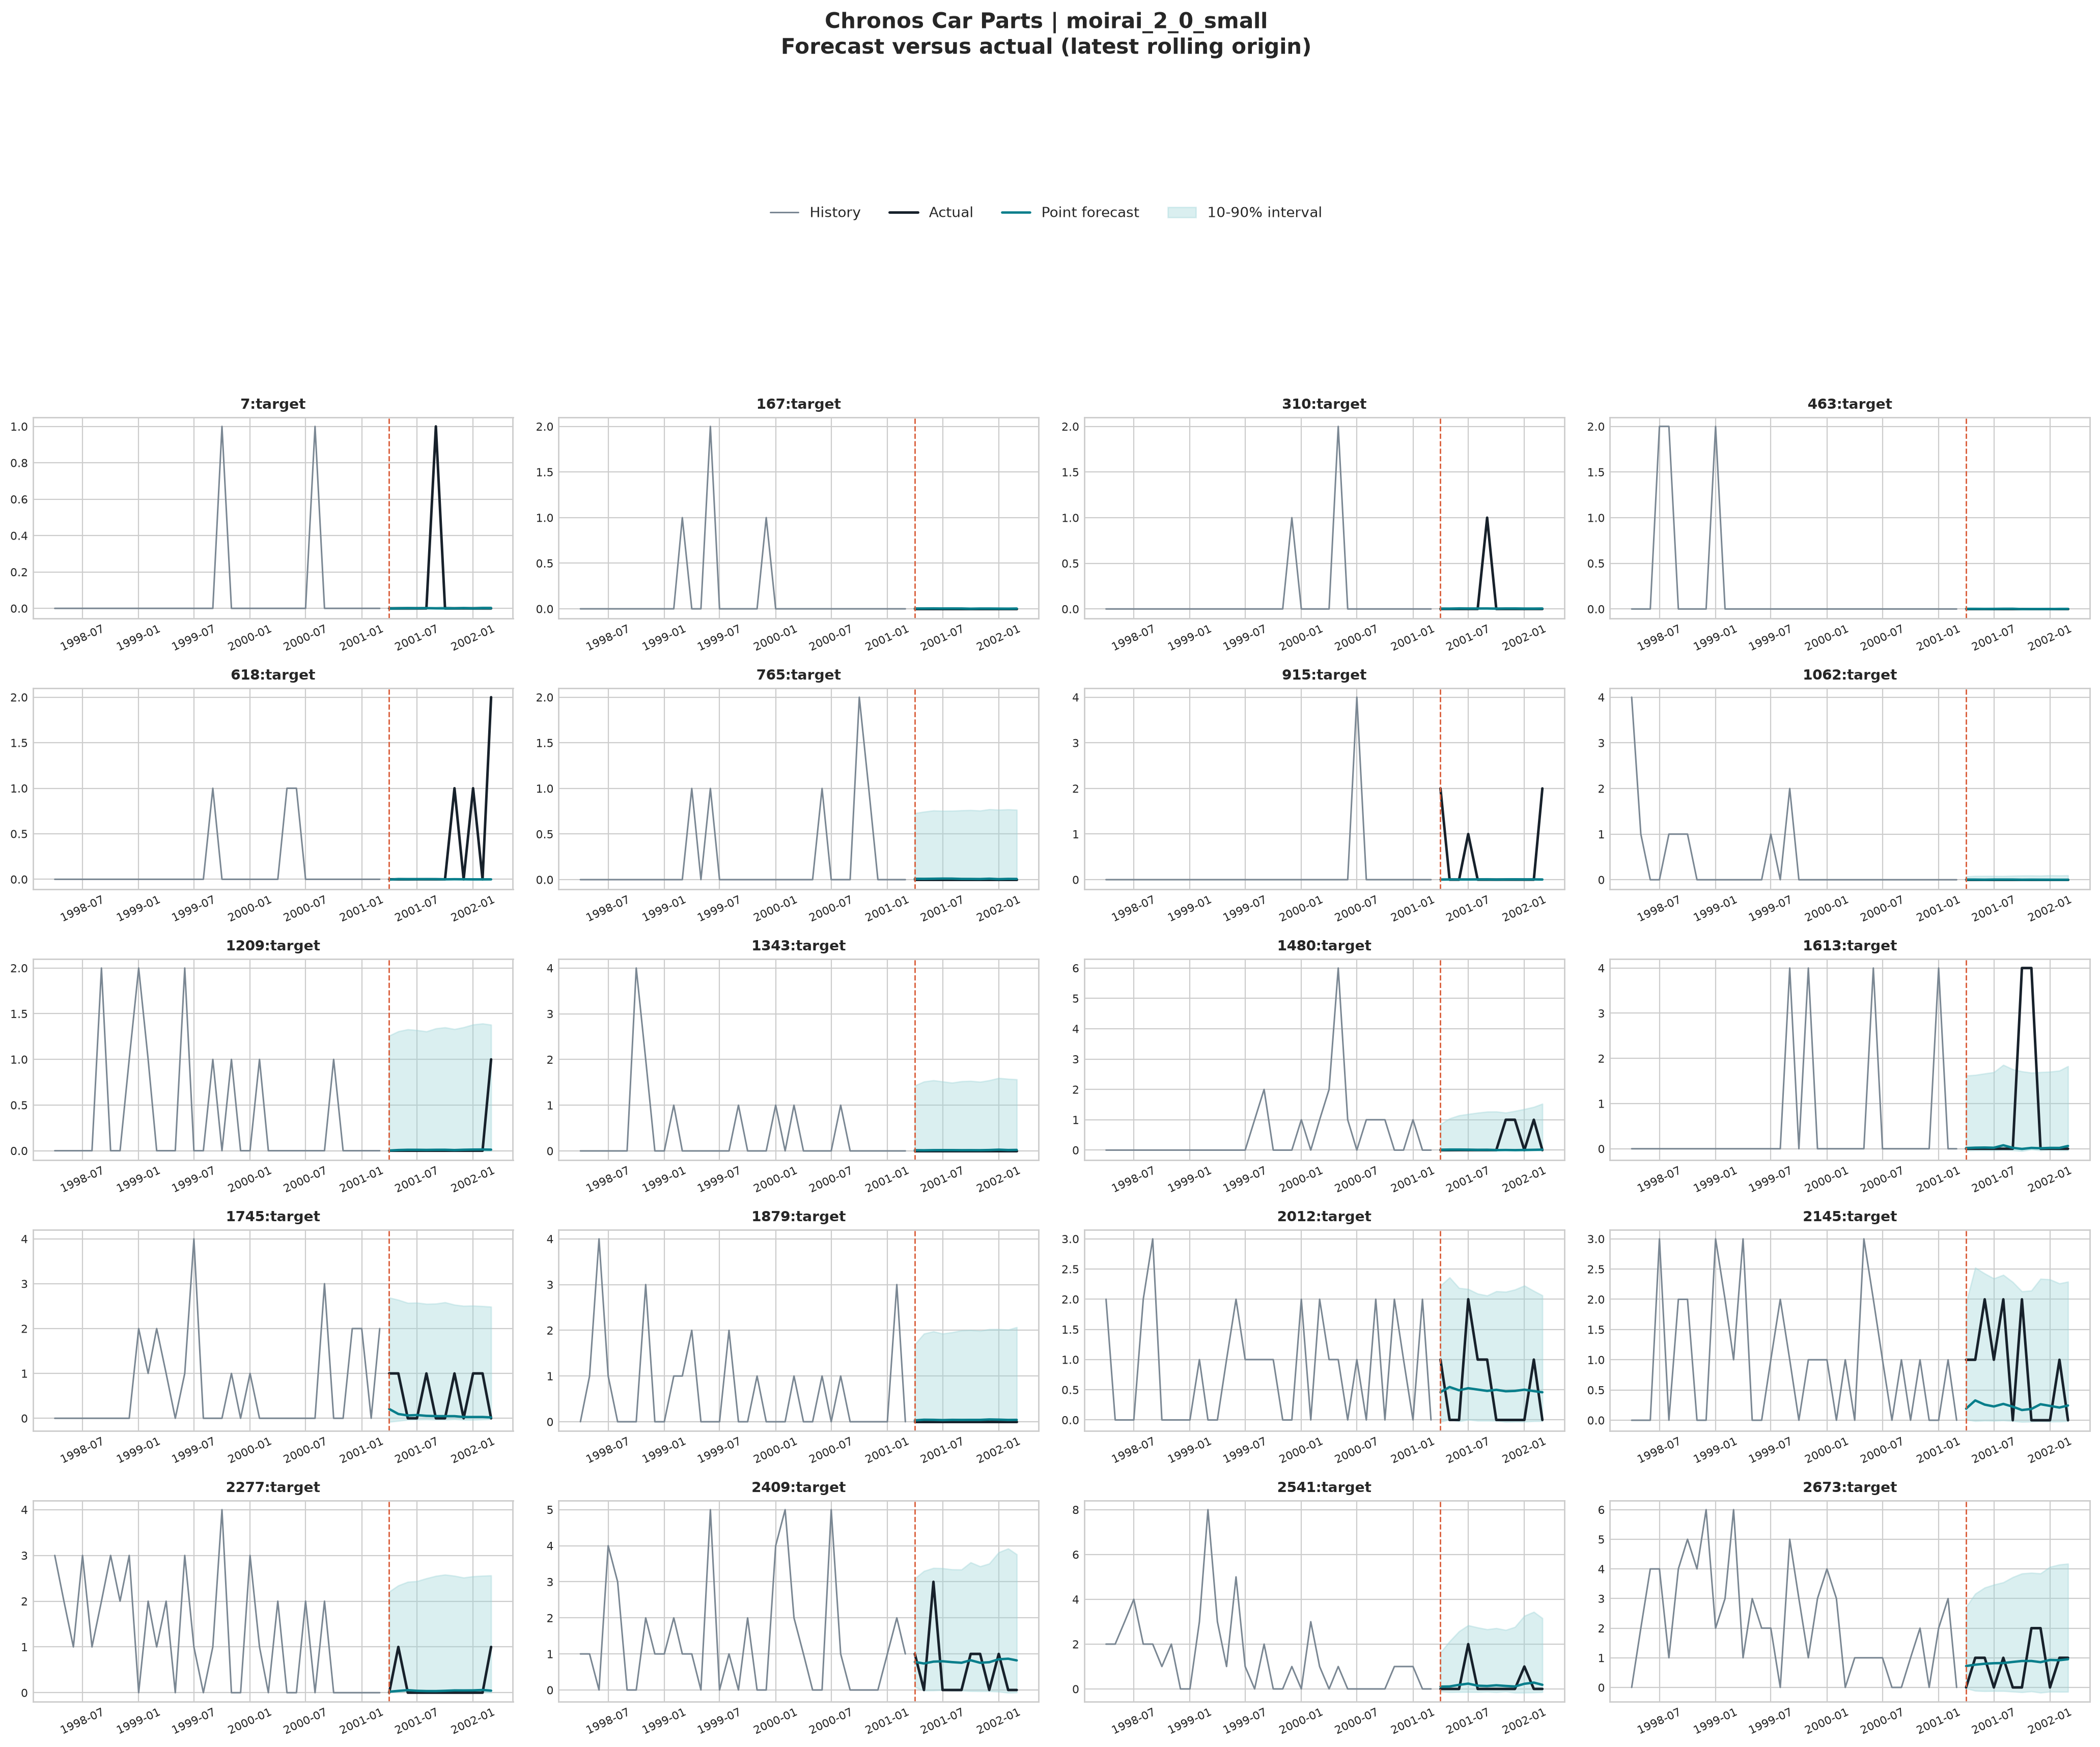
\includegraphics[width=\linewidth,height=0.79\textheight,keepaspectratio]{chronos_car_parts/forecast_vs_actual/moirai_2_0_small.png}
\end{frame}

% ------------------------------------------------------------
\begin{frame}{Car Parts --- forecast vs. actual --- Seasonal Naive}
  \centering
  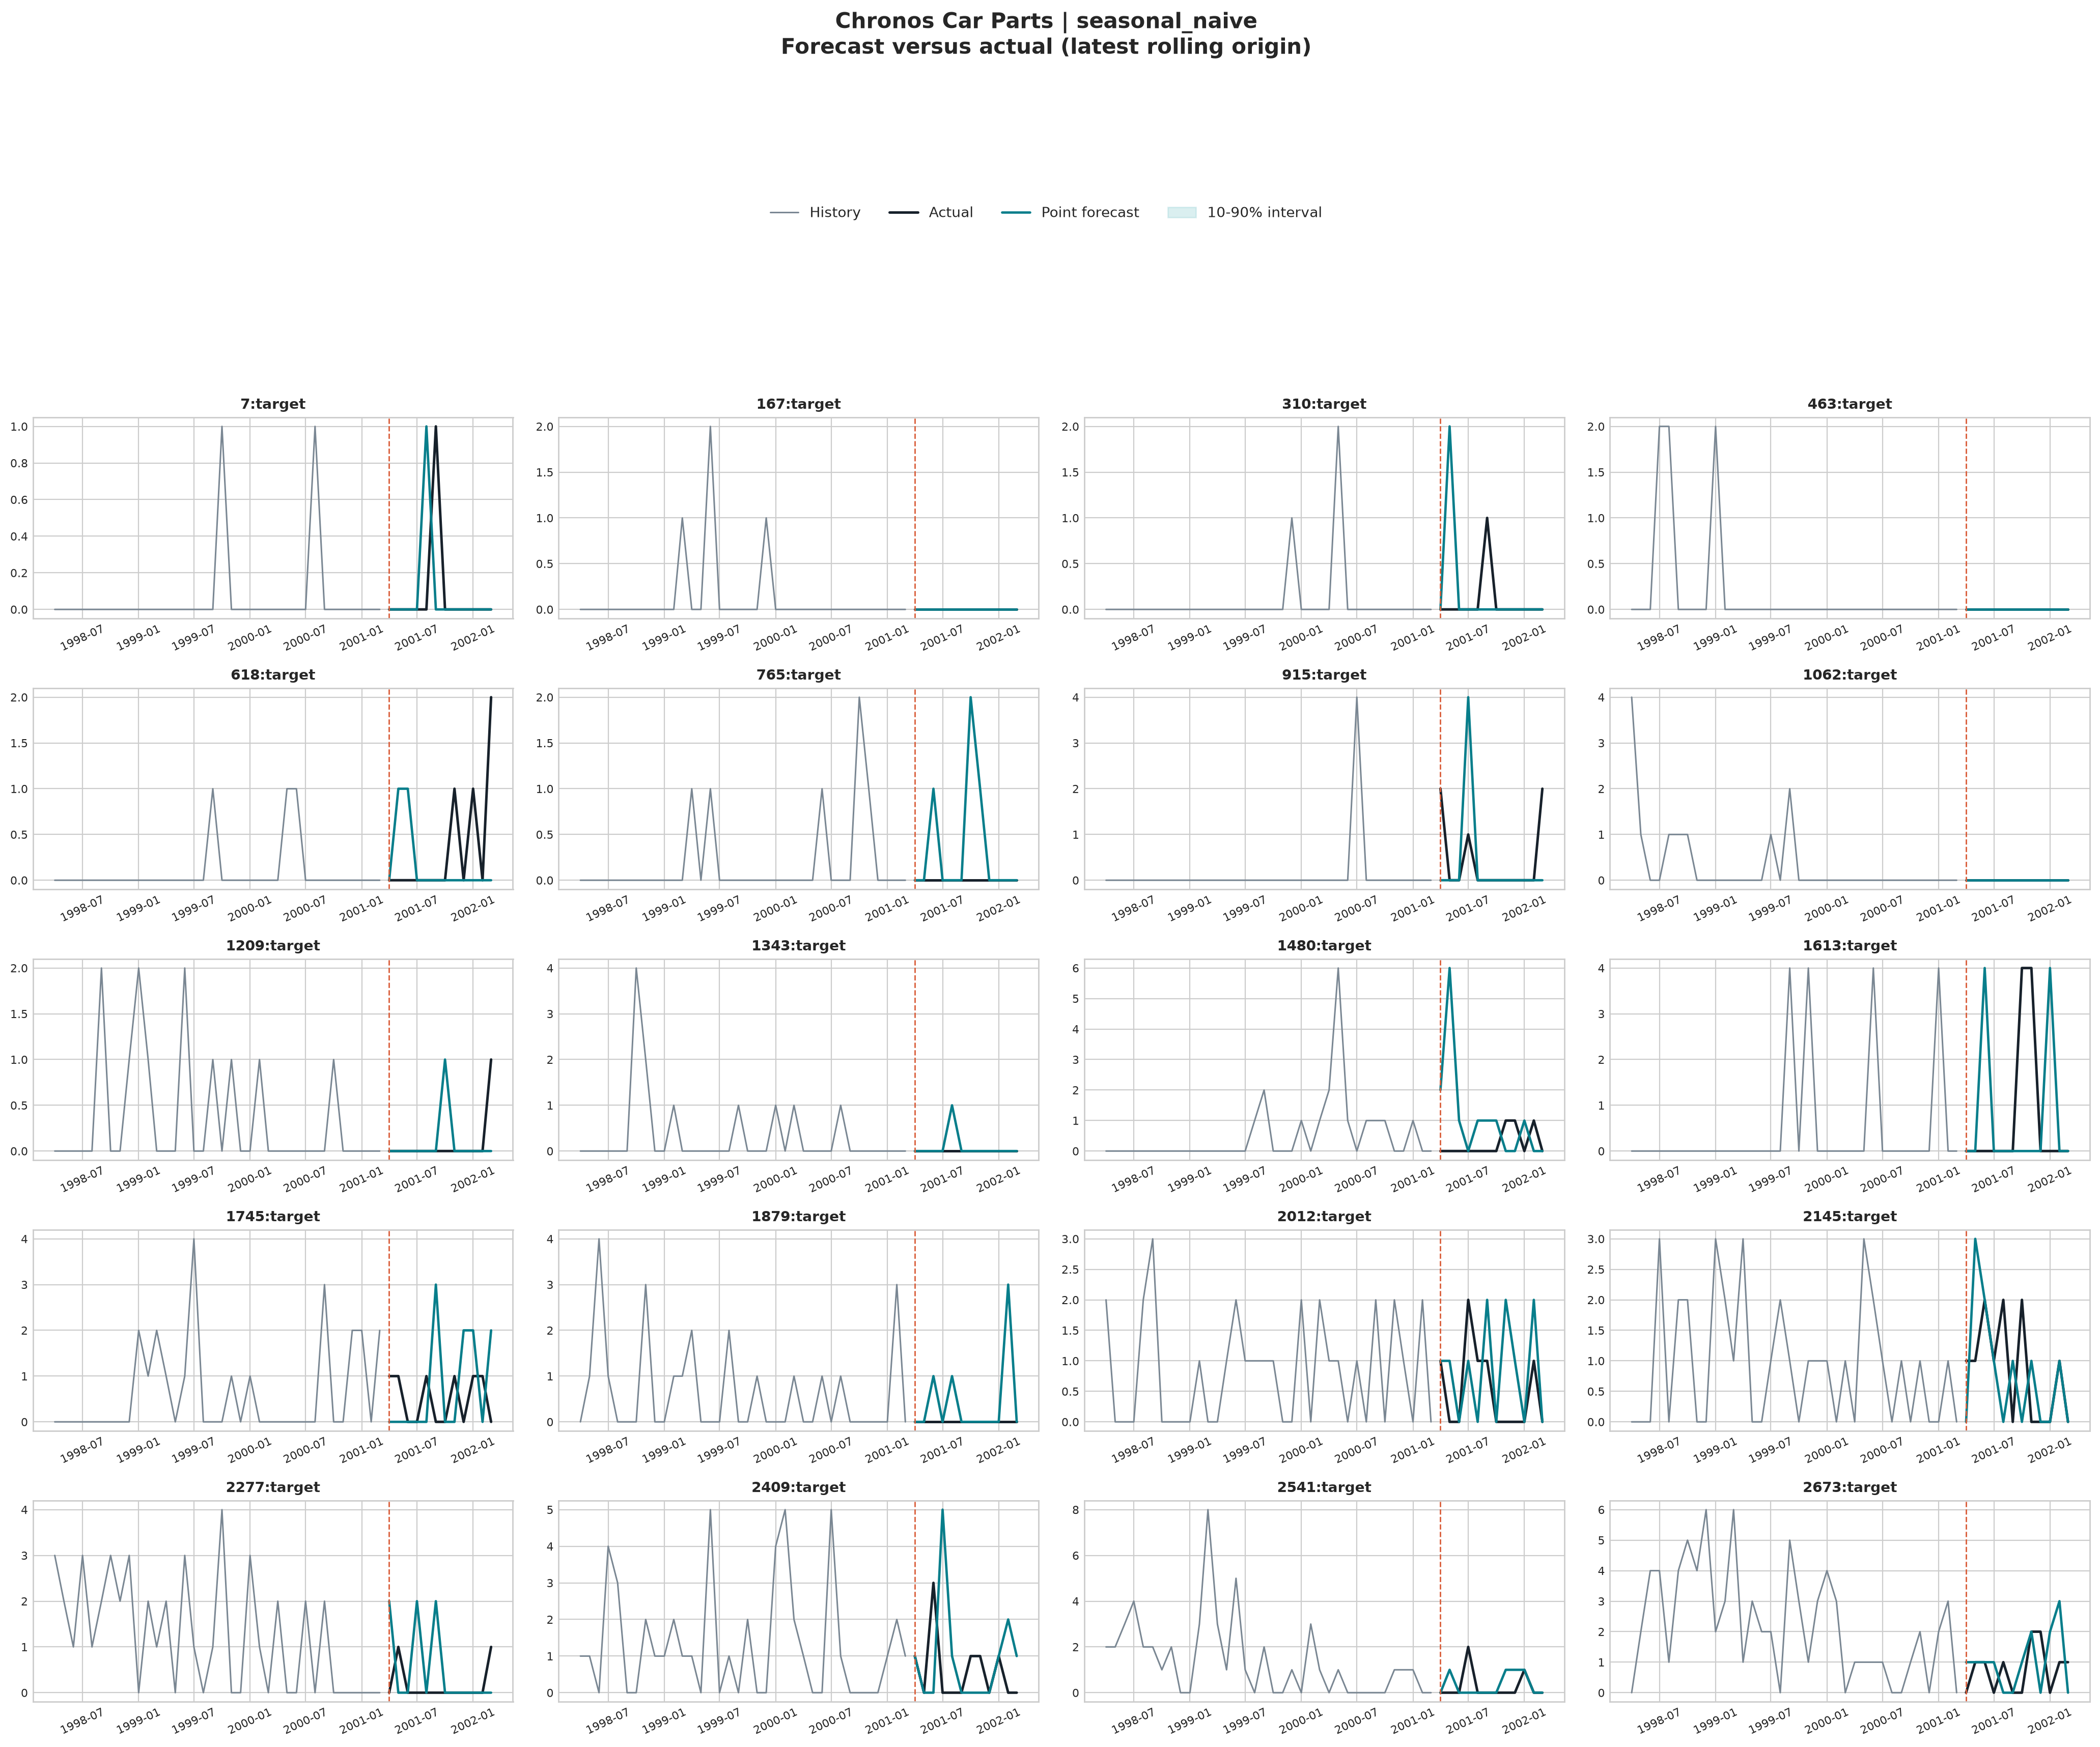
\includegraphics[width=\linewidth,height=0.79\textheight,keepaspectratio]{chronos_car_parts/forecast_vs_actual/seasonal_naive.png}
\end{frame}

% ------------------------------------------------------------
\begin{frame}{Car Parts --- forecast vs. actual --- ARIMA(2,1,2)}
  \centering
  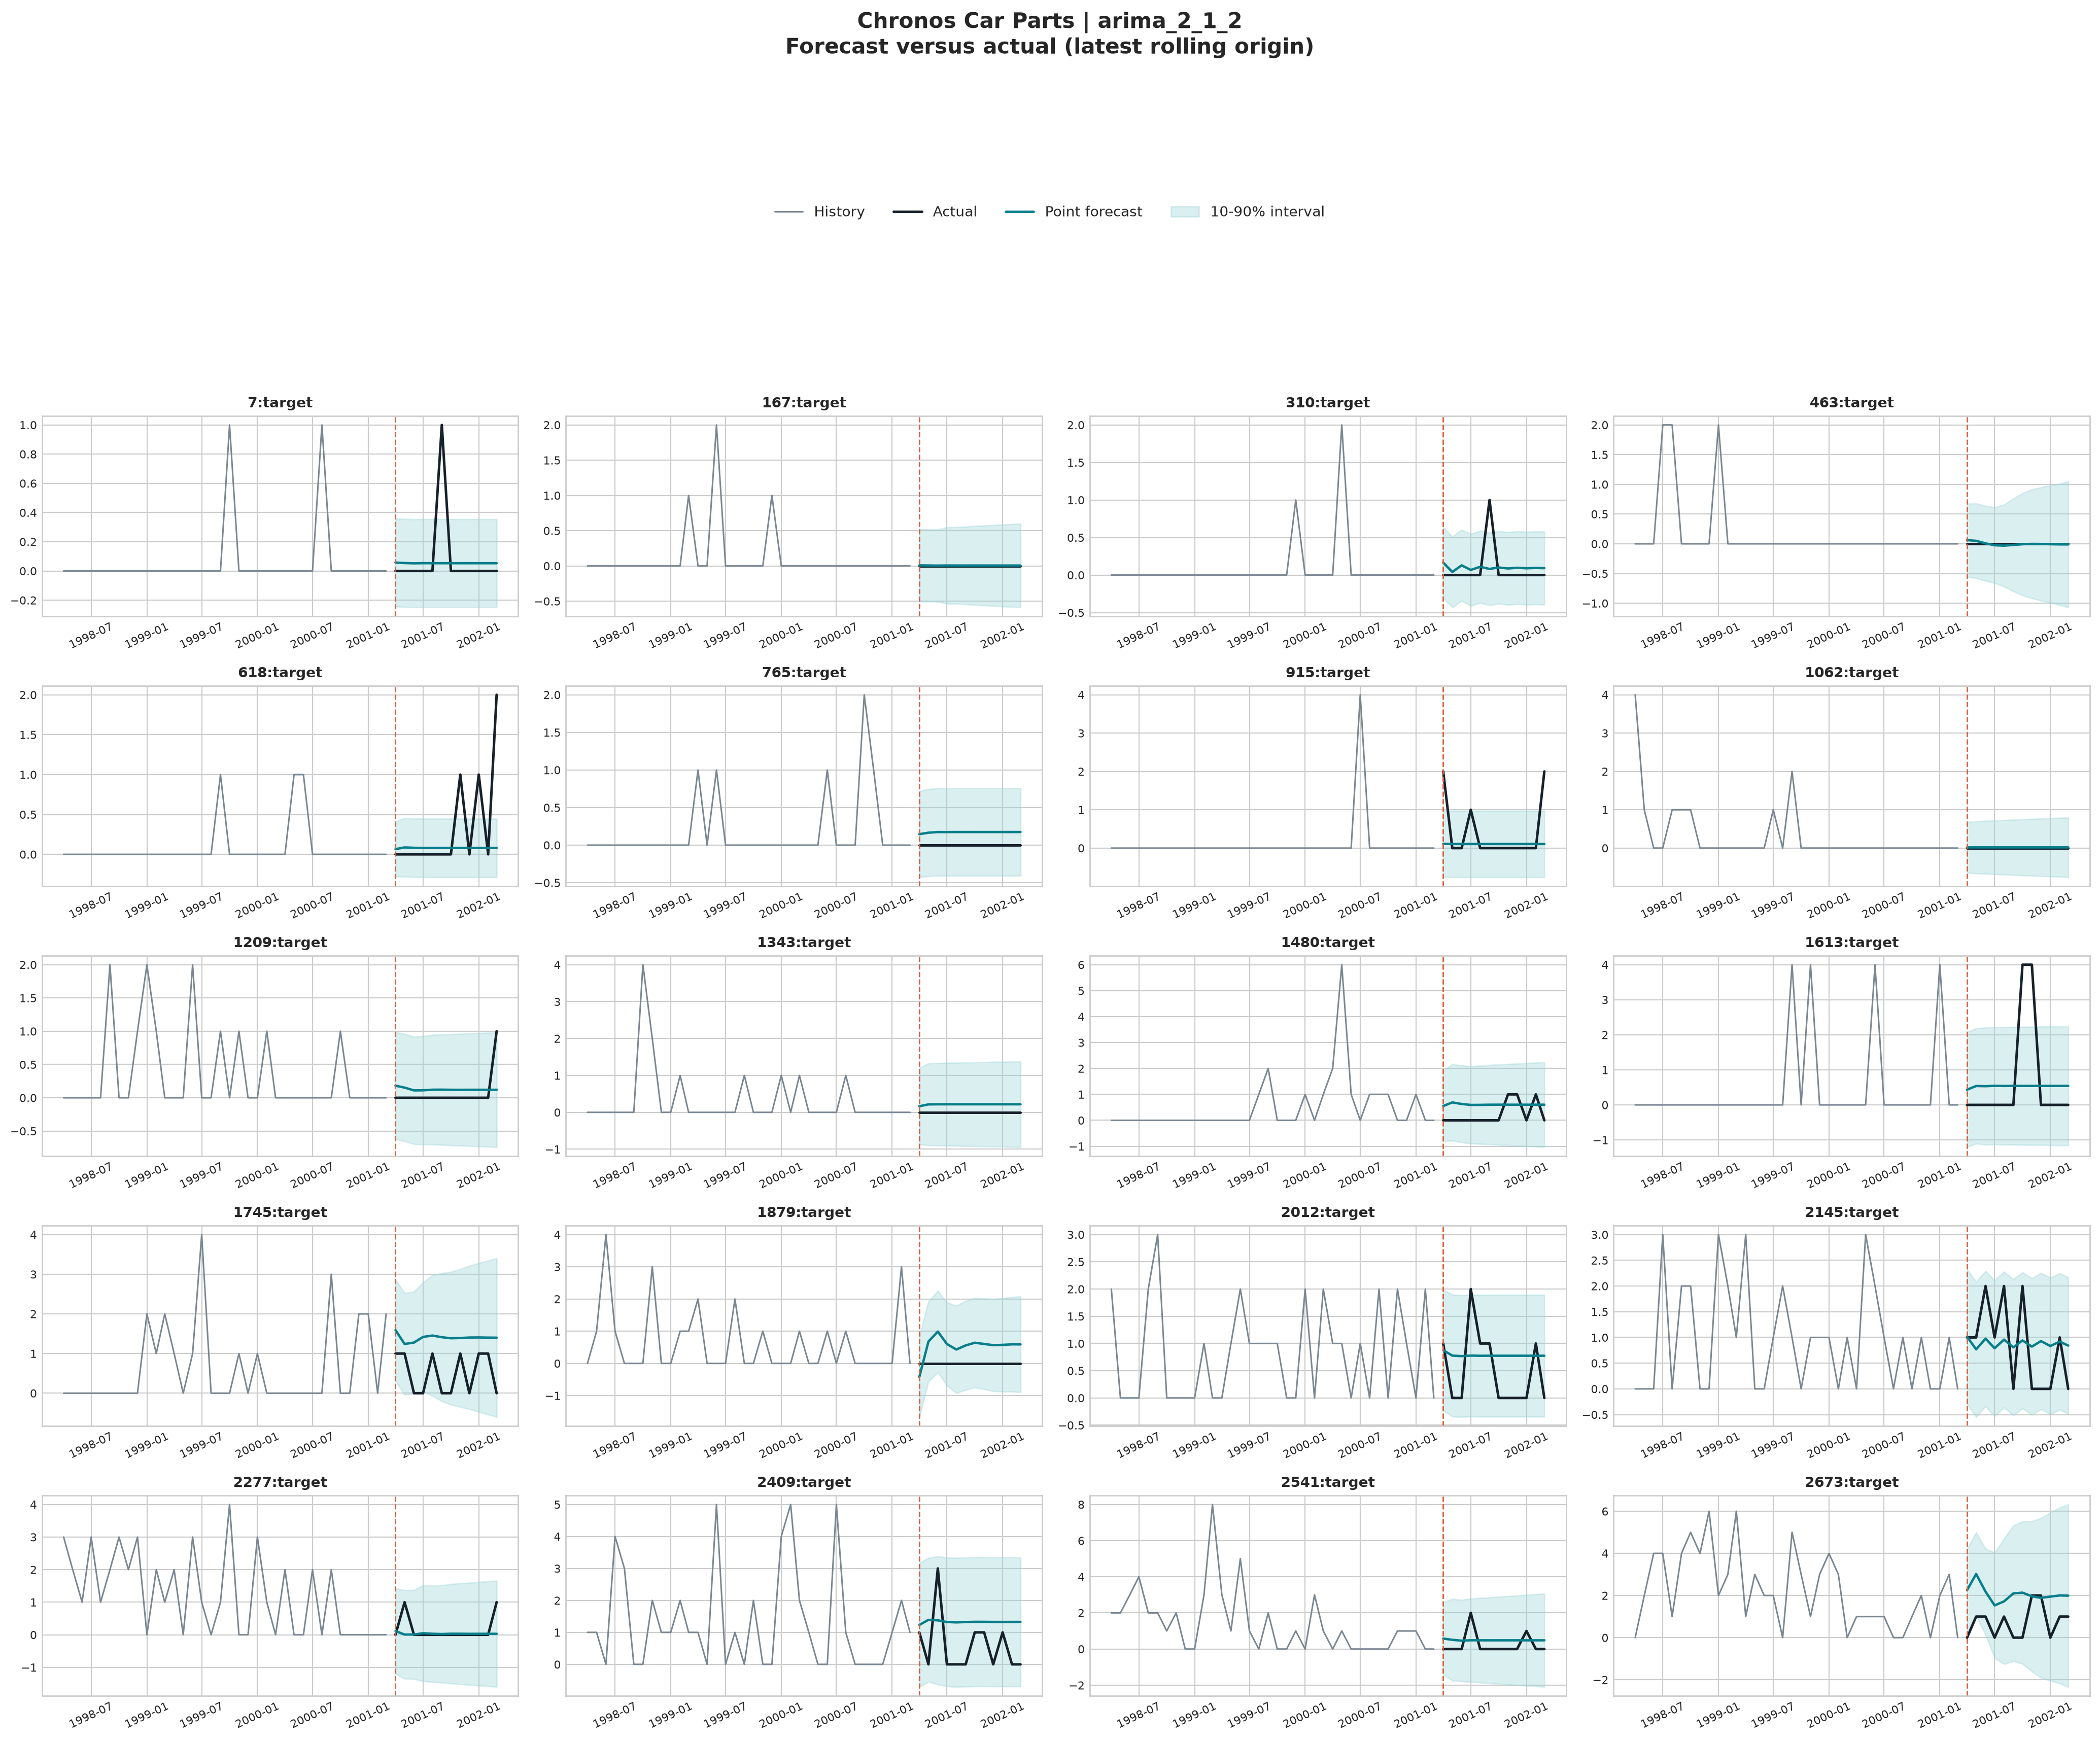
\includegraphics[width=\linewidth,height=0.79\textheight,keepaspectratio]{chronos_car_parts/forecast_vs_actual/arima_2_1_2.png}
\end{frame}

% ------------------------------------------------------------
\begin{frame}{Car Parts --- forecast vs. actual --- AutoARIMA}
  \centering
  
\includegraphics[width=\linewidth,height=0.79\textheight,keepaspectratio]{chronos_car_parts/forecast_vs_actual/auto_arima.png}
\end{frame}

% ------------------------------------------------------------
\begin{frame}{Car Parts --- forecast vs. actual --- Prophet}
  \centering
  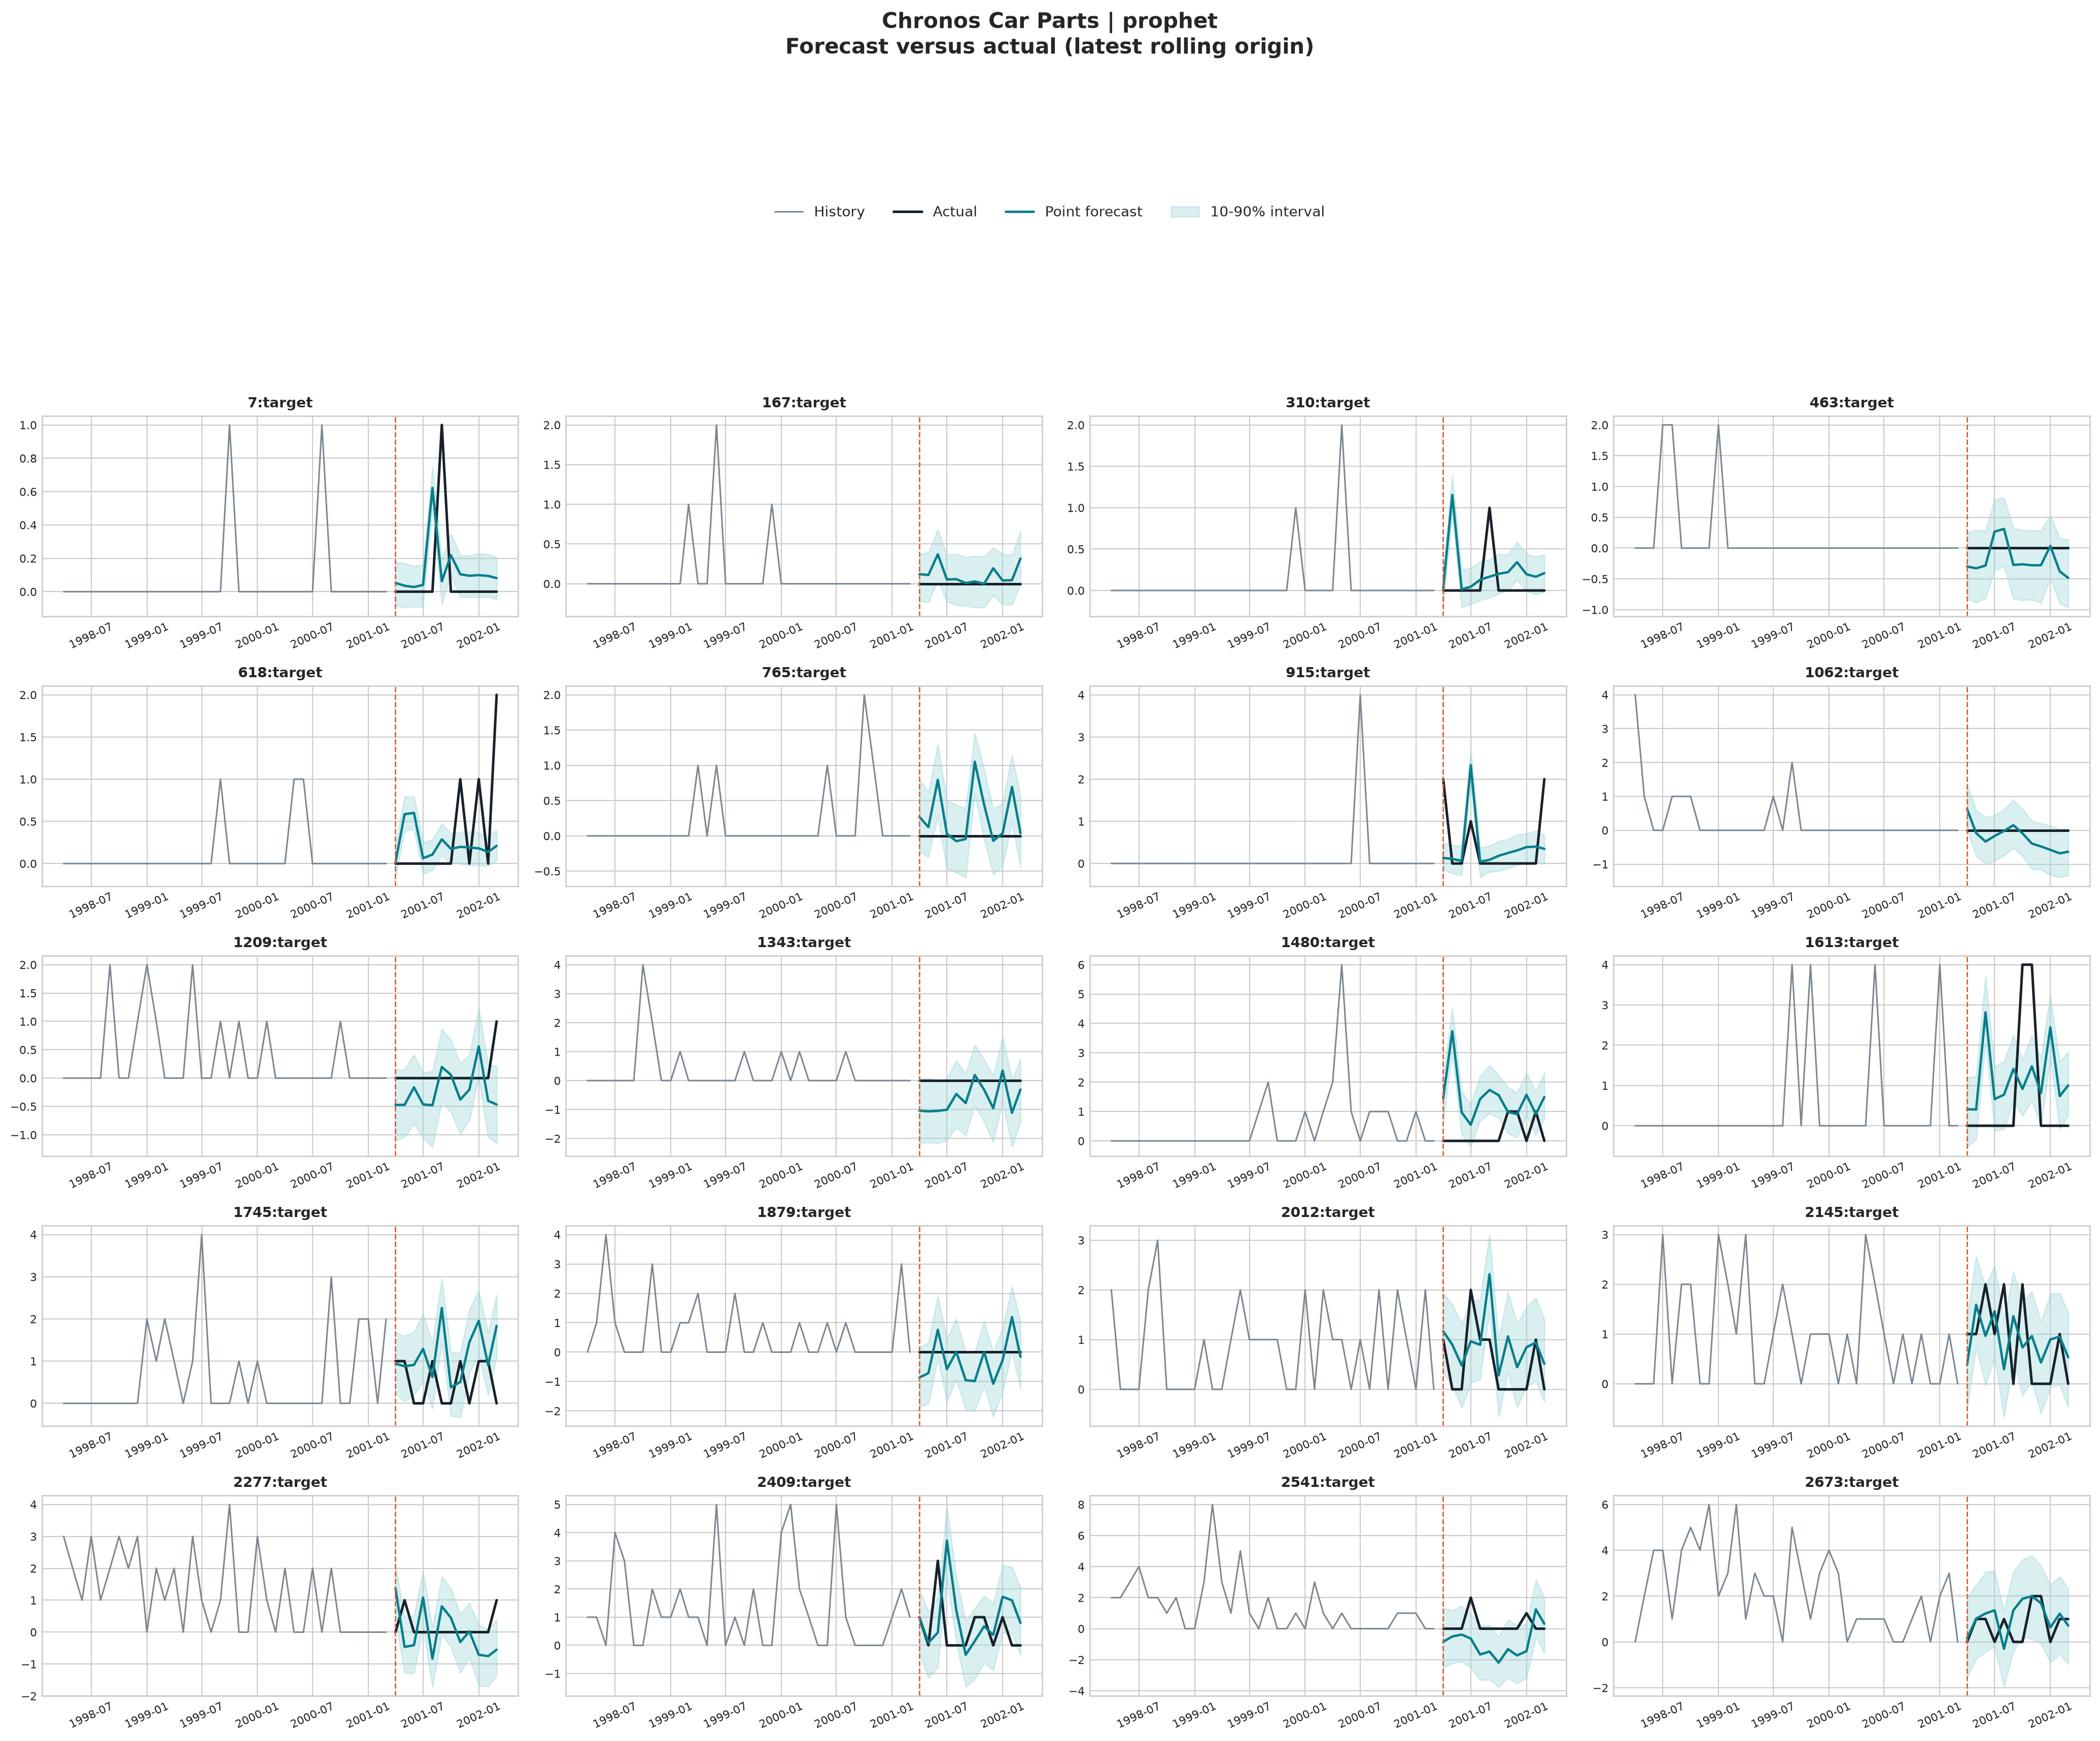
\includegraphics[width=\linewidth,height=0.79\textheight,keepaspectratio]{chronos_car_parts/forecast_vs_actual/prophet.png}
\end{frame}

% ------------------------------------------------------------
\begin{frame}{Car Parts --- forecast vs. actual --- DeepAR}
  \centering
  
\includegraphics[width=\linewidth,height=0.79\textheight,keepaspectratio]{chronos_car_parts/forecast_vs_actual/deepar.png}
\end{frame}

% ------------------------------------------------------------
\begin{frame}{Car Parts --- forecast vs. actual --- Chronos Mini}
  \centering
  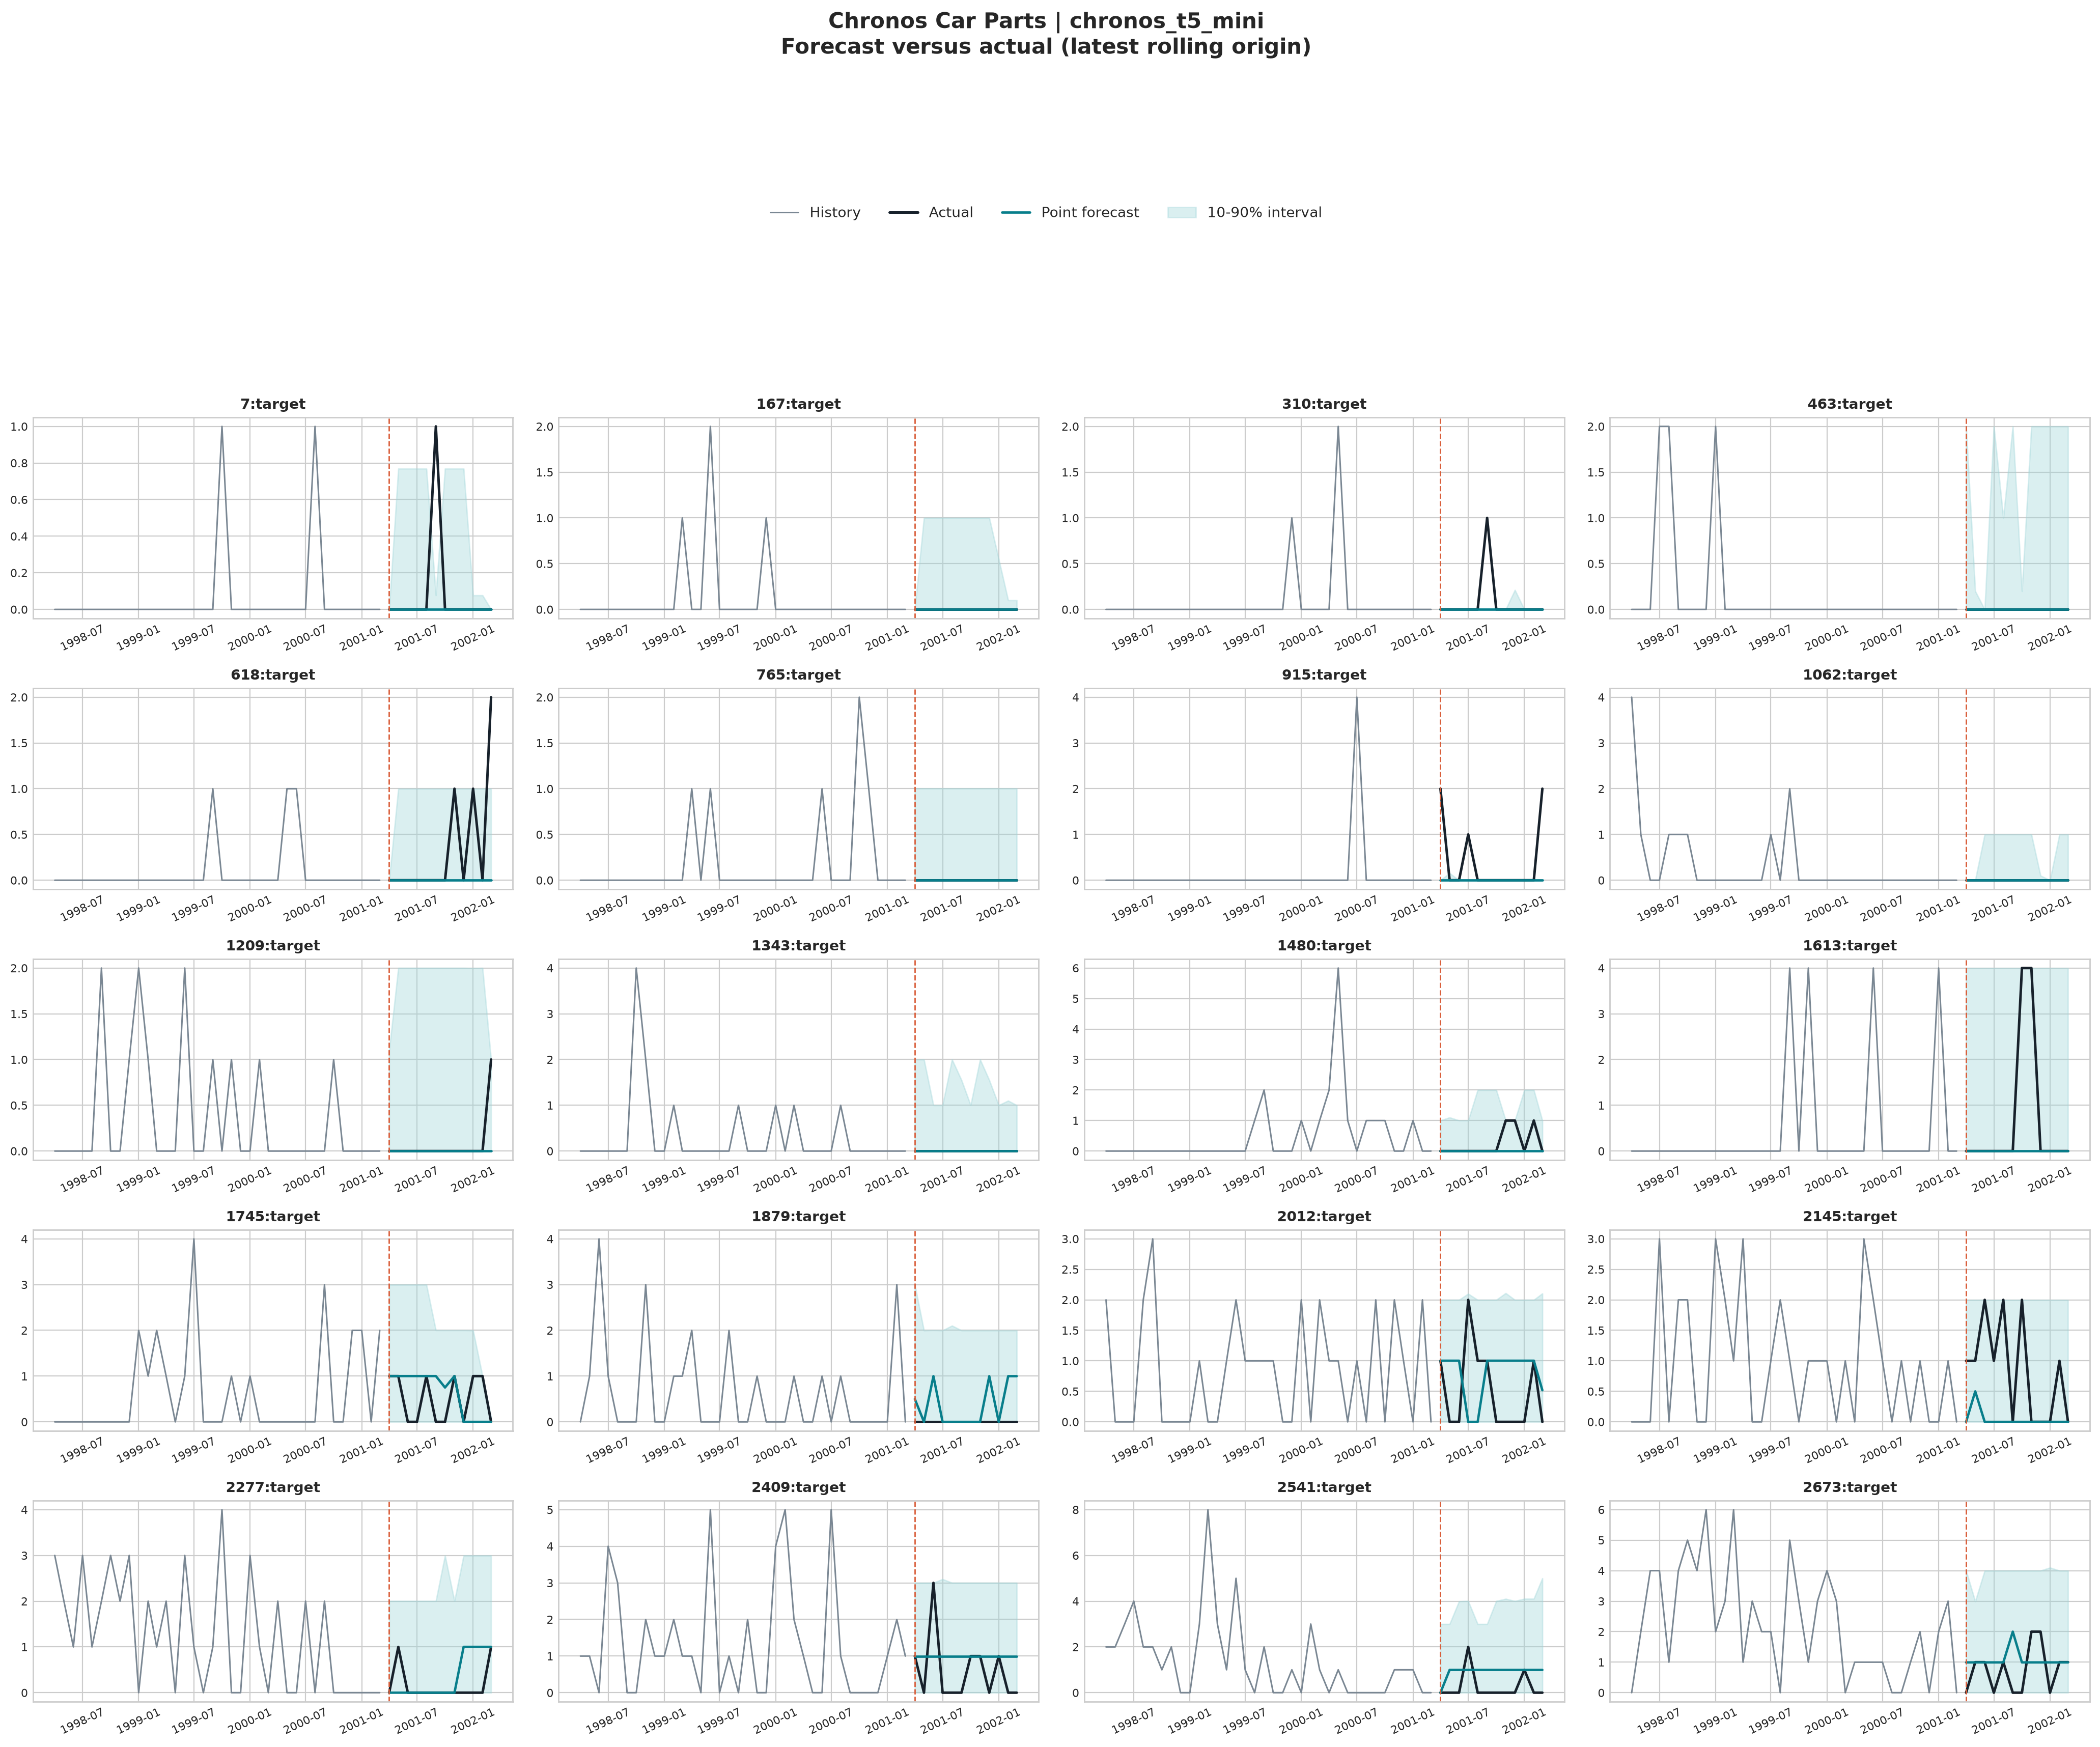
\includegraphics[width=\linewidth,height=0.79\textheight,keepaspectratio]{chronos_car_parts/forecast_vs_actual/chronos_t5_mini.png}
\end{frame}

% ------------------------------------------------------------
\begin{frame}{Car Parts --- forecast vs. actual --- Chronos Small}
  \centering
  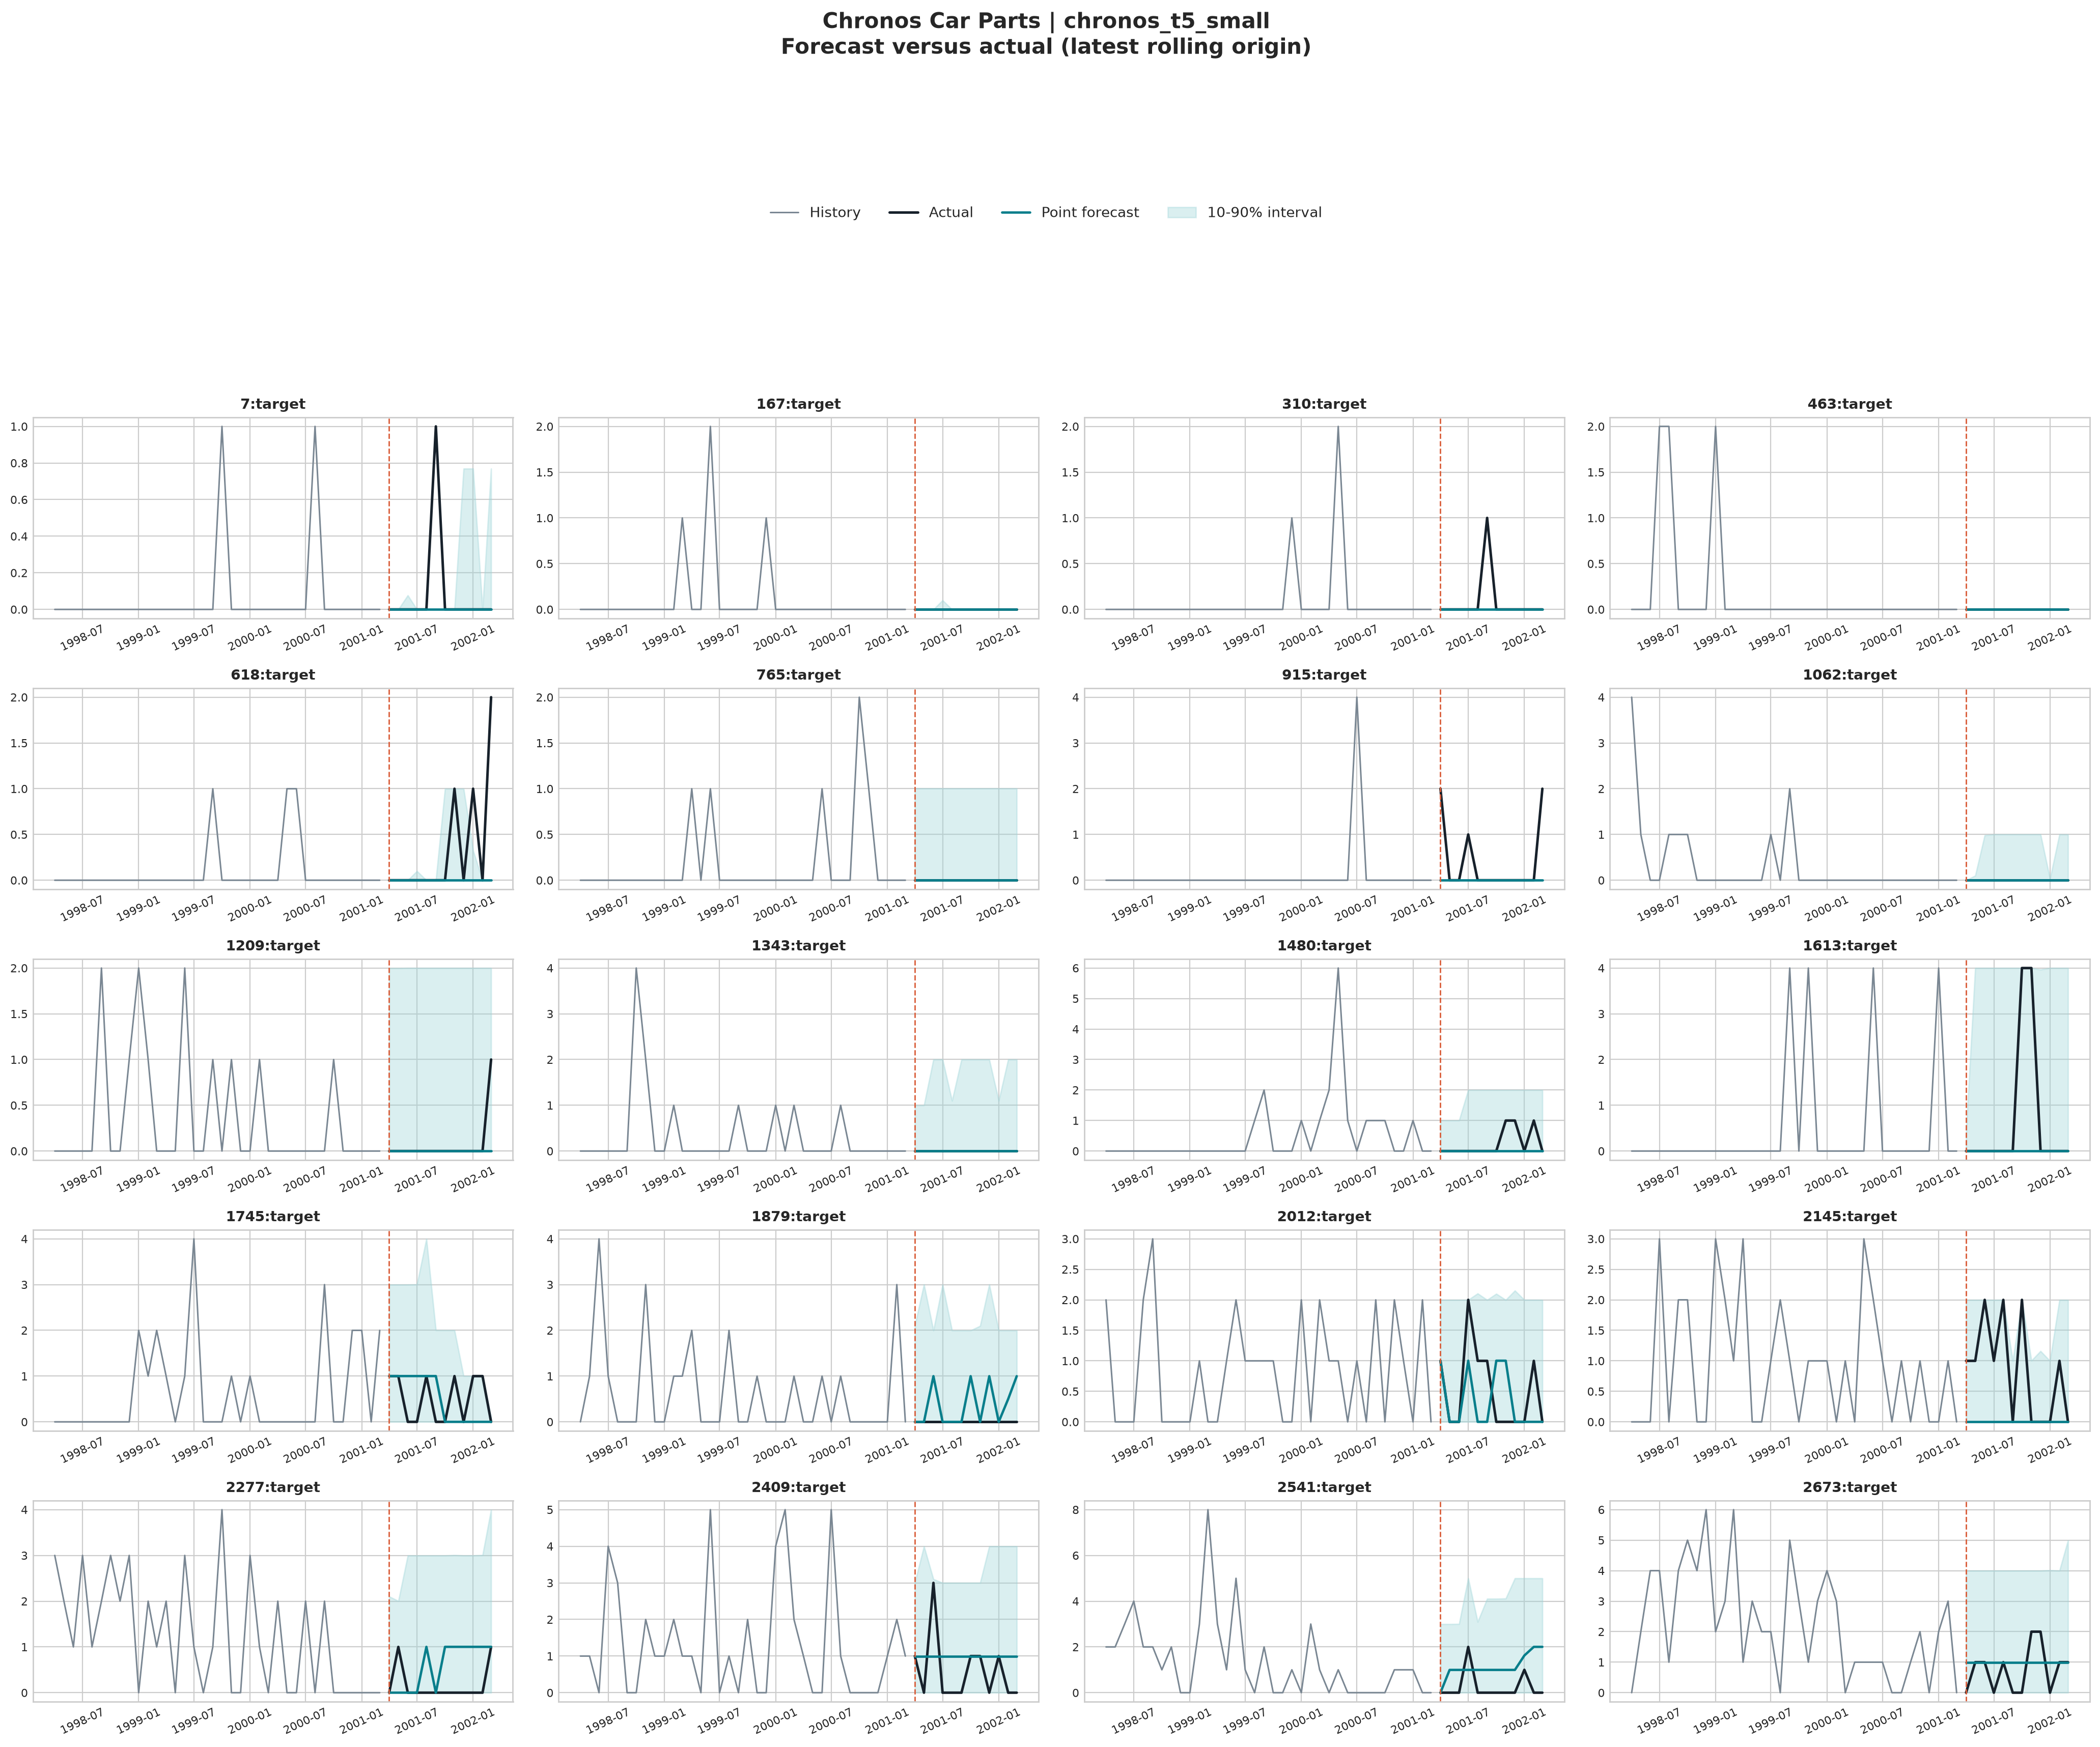
\includegraphics[width=\linewidth,height=0.79\textheight,keepaspectratio]{chronos_car_parts/forecast_vs_actual/chronos_t5_small.png}
\end{frame}

% ------------------------------------------------------------
\begin{frame}{Car Parts --- forecast vs. actual --- Chronos Base}
  \centering
  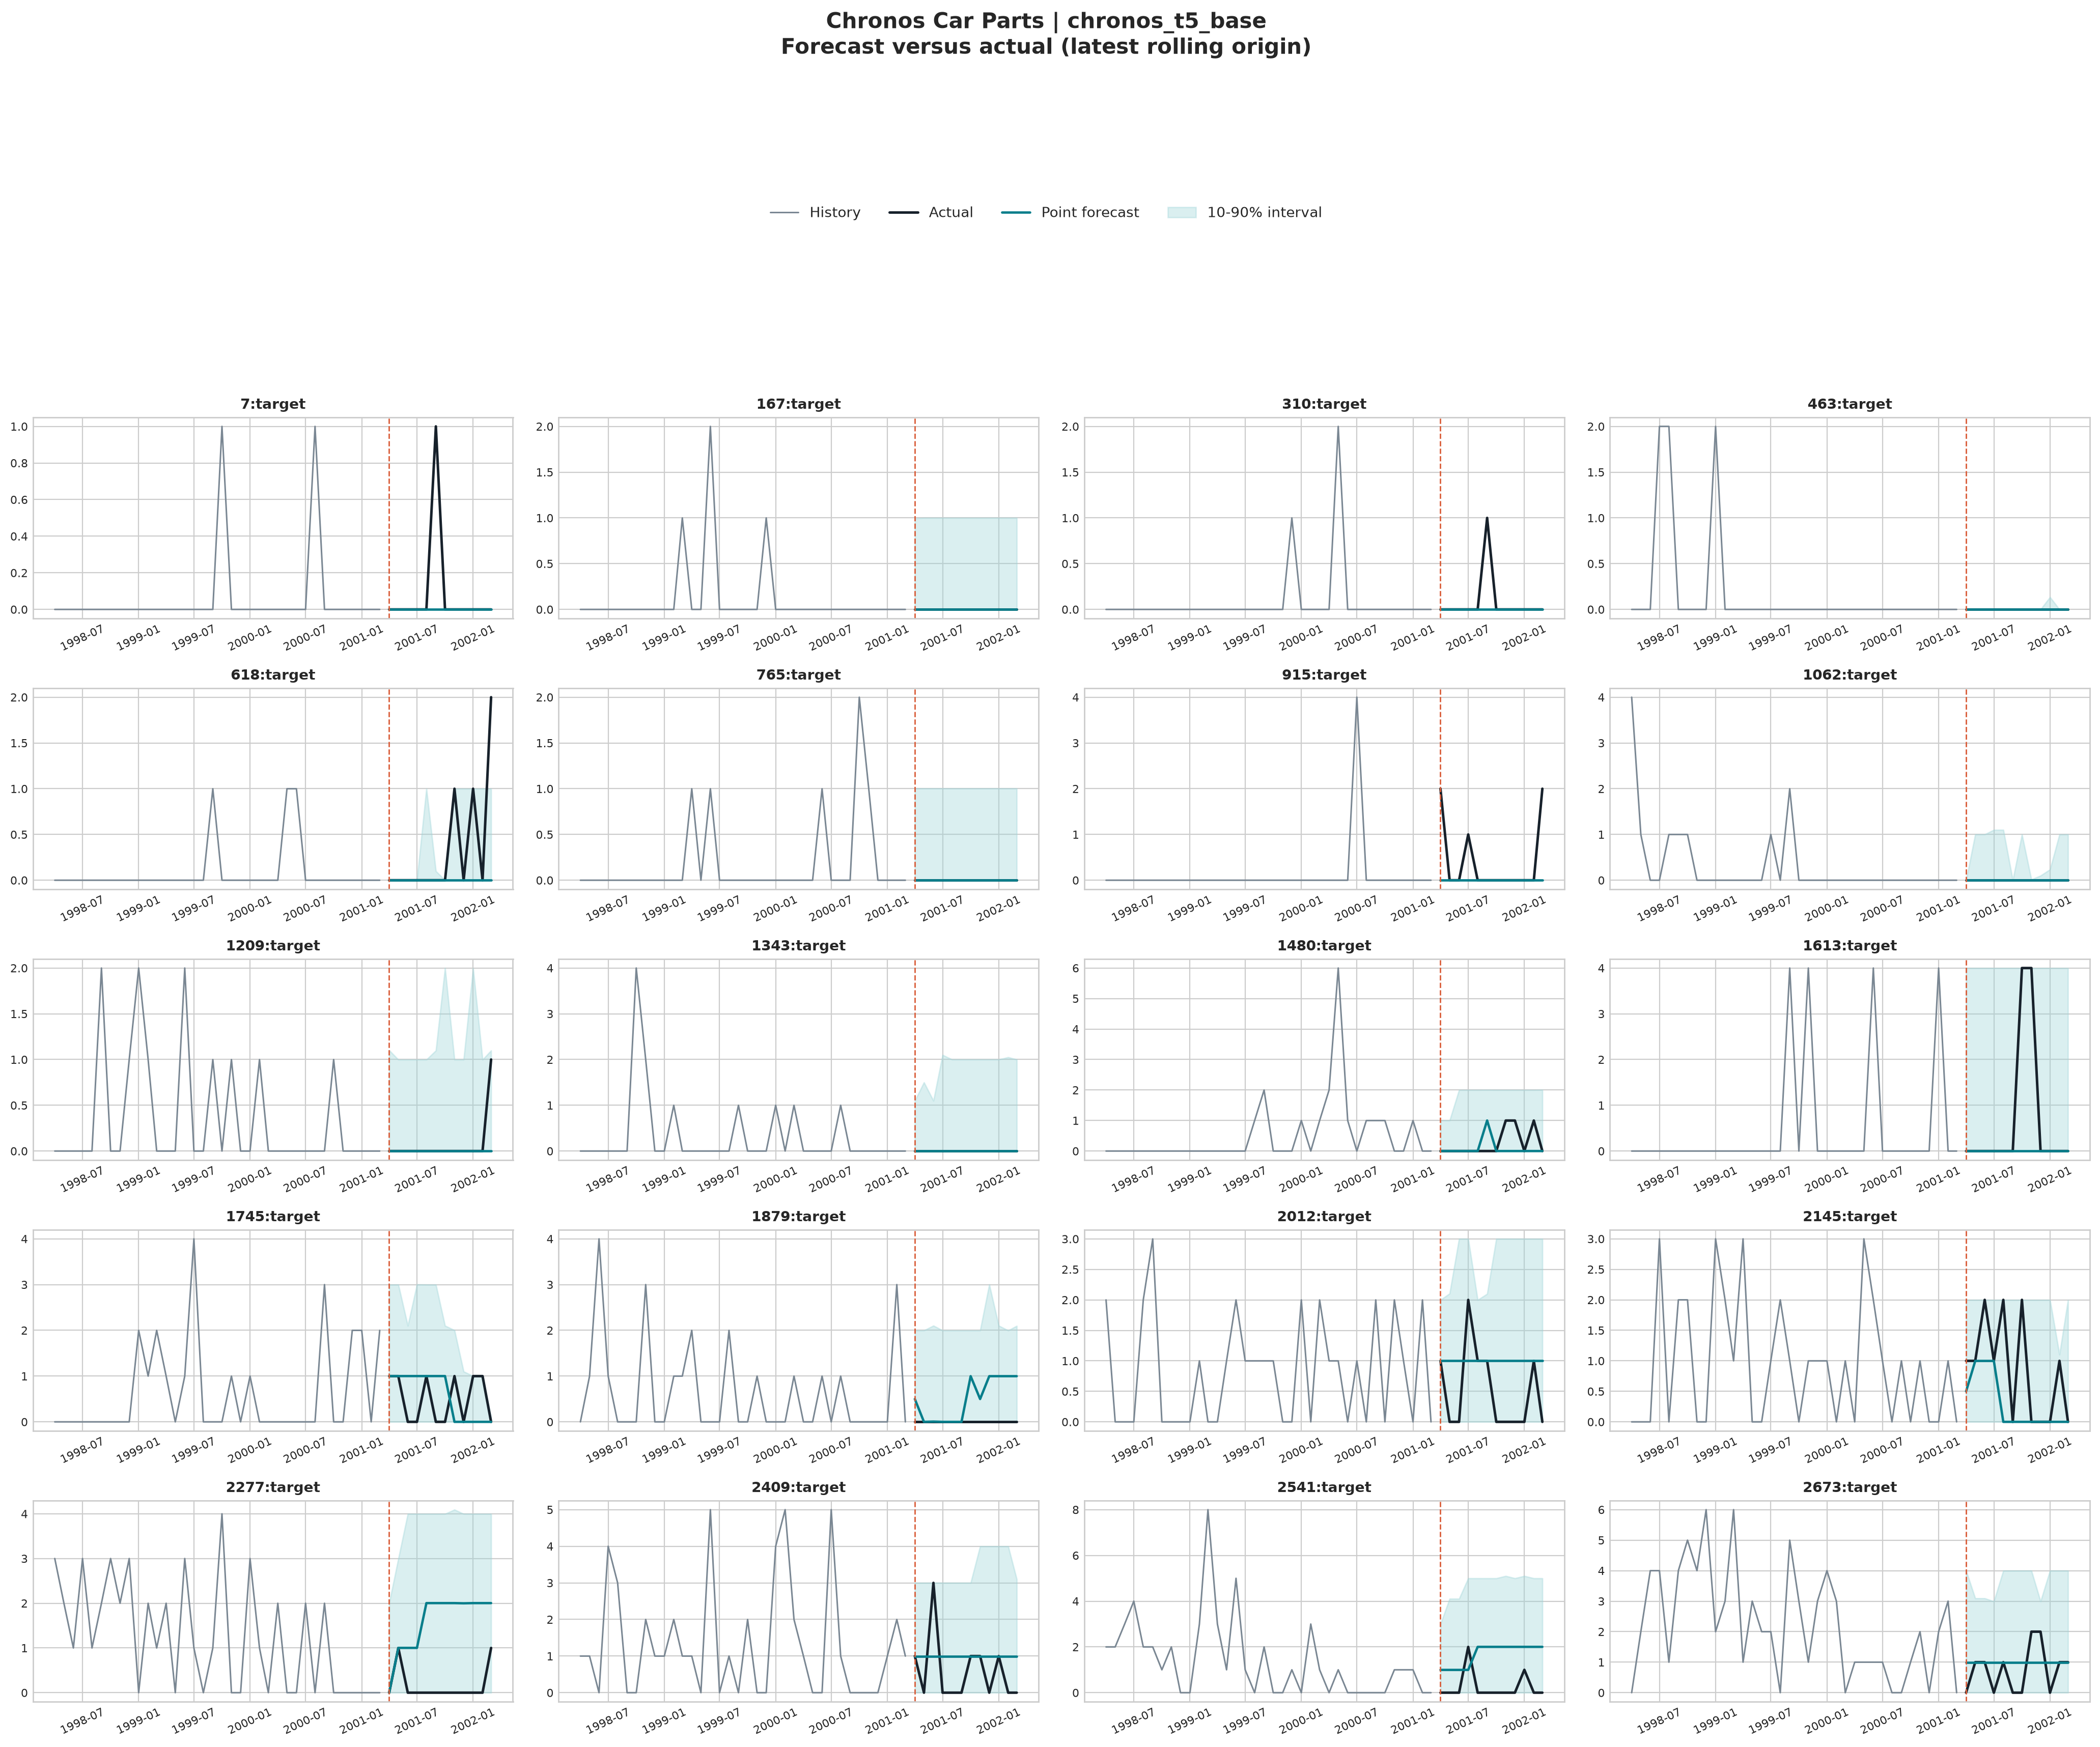
\includegraphics[width=\linewidth,height=0.79\textheight,keepaspectratio]{chronos_car_parts/forecast_vs_actual/chronos_t5_base.png}
\end{frame}

% ------------------------------------------------------------
\begin{frame}{Car Parts --- forecast vs. actual --- Chronos Large}
  \centering
  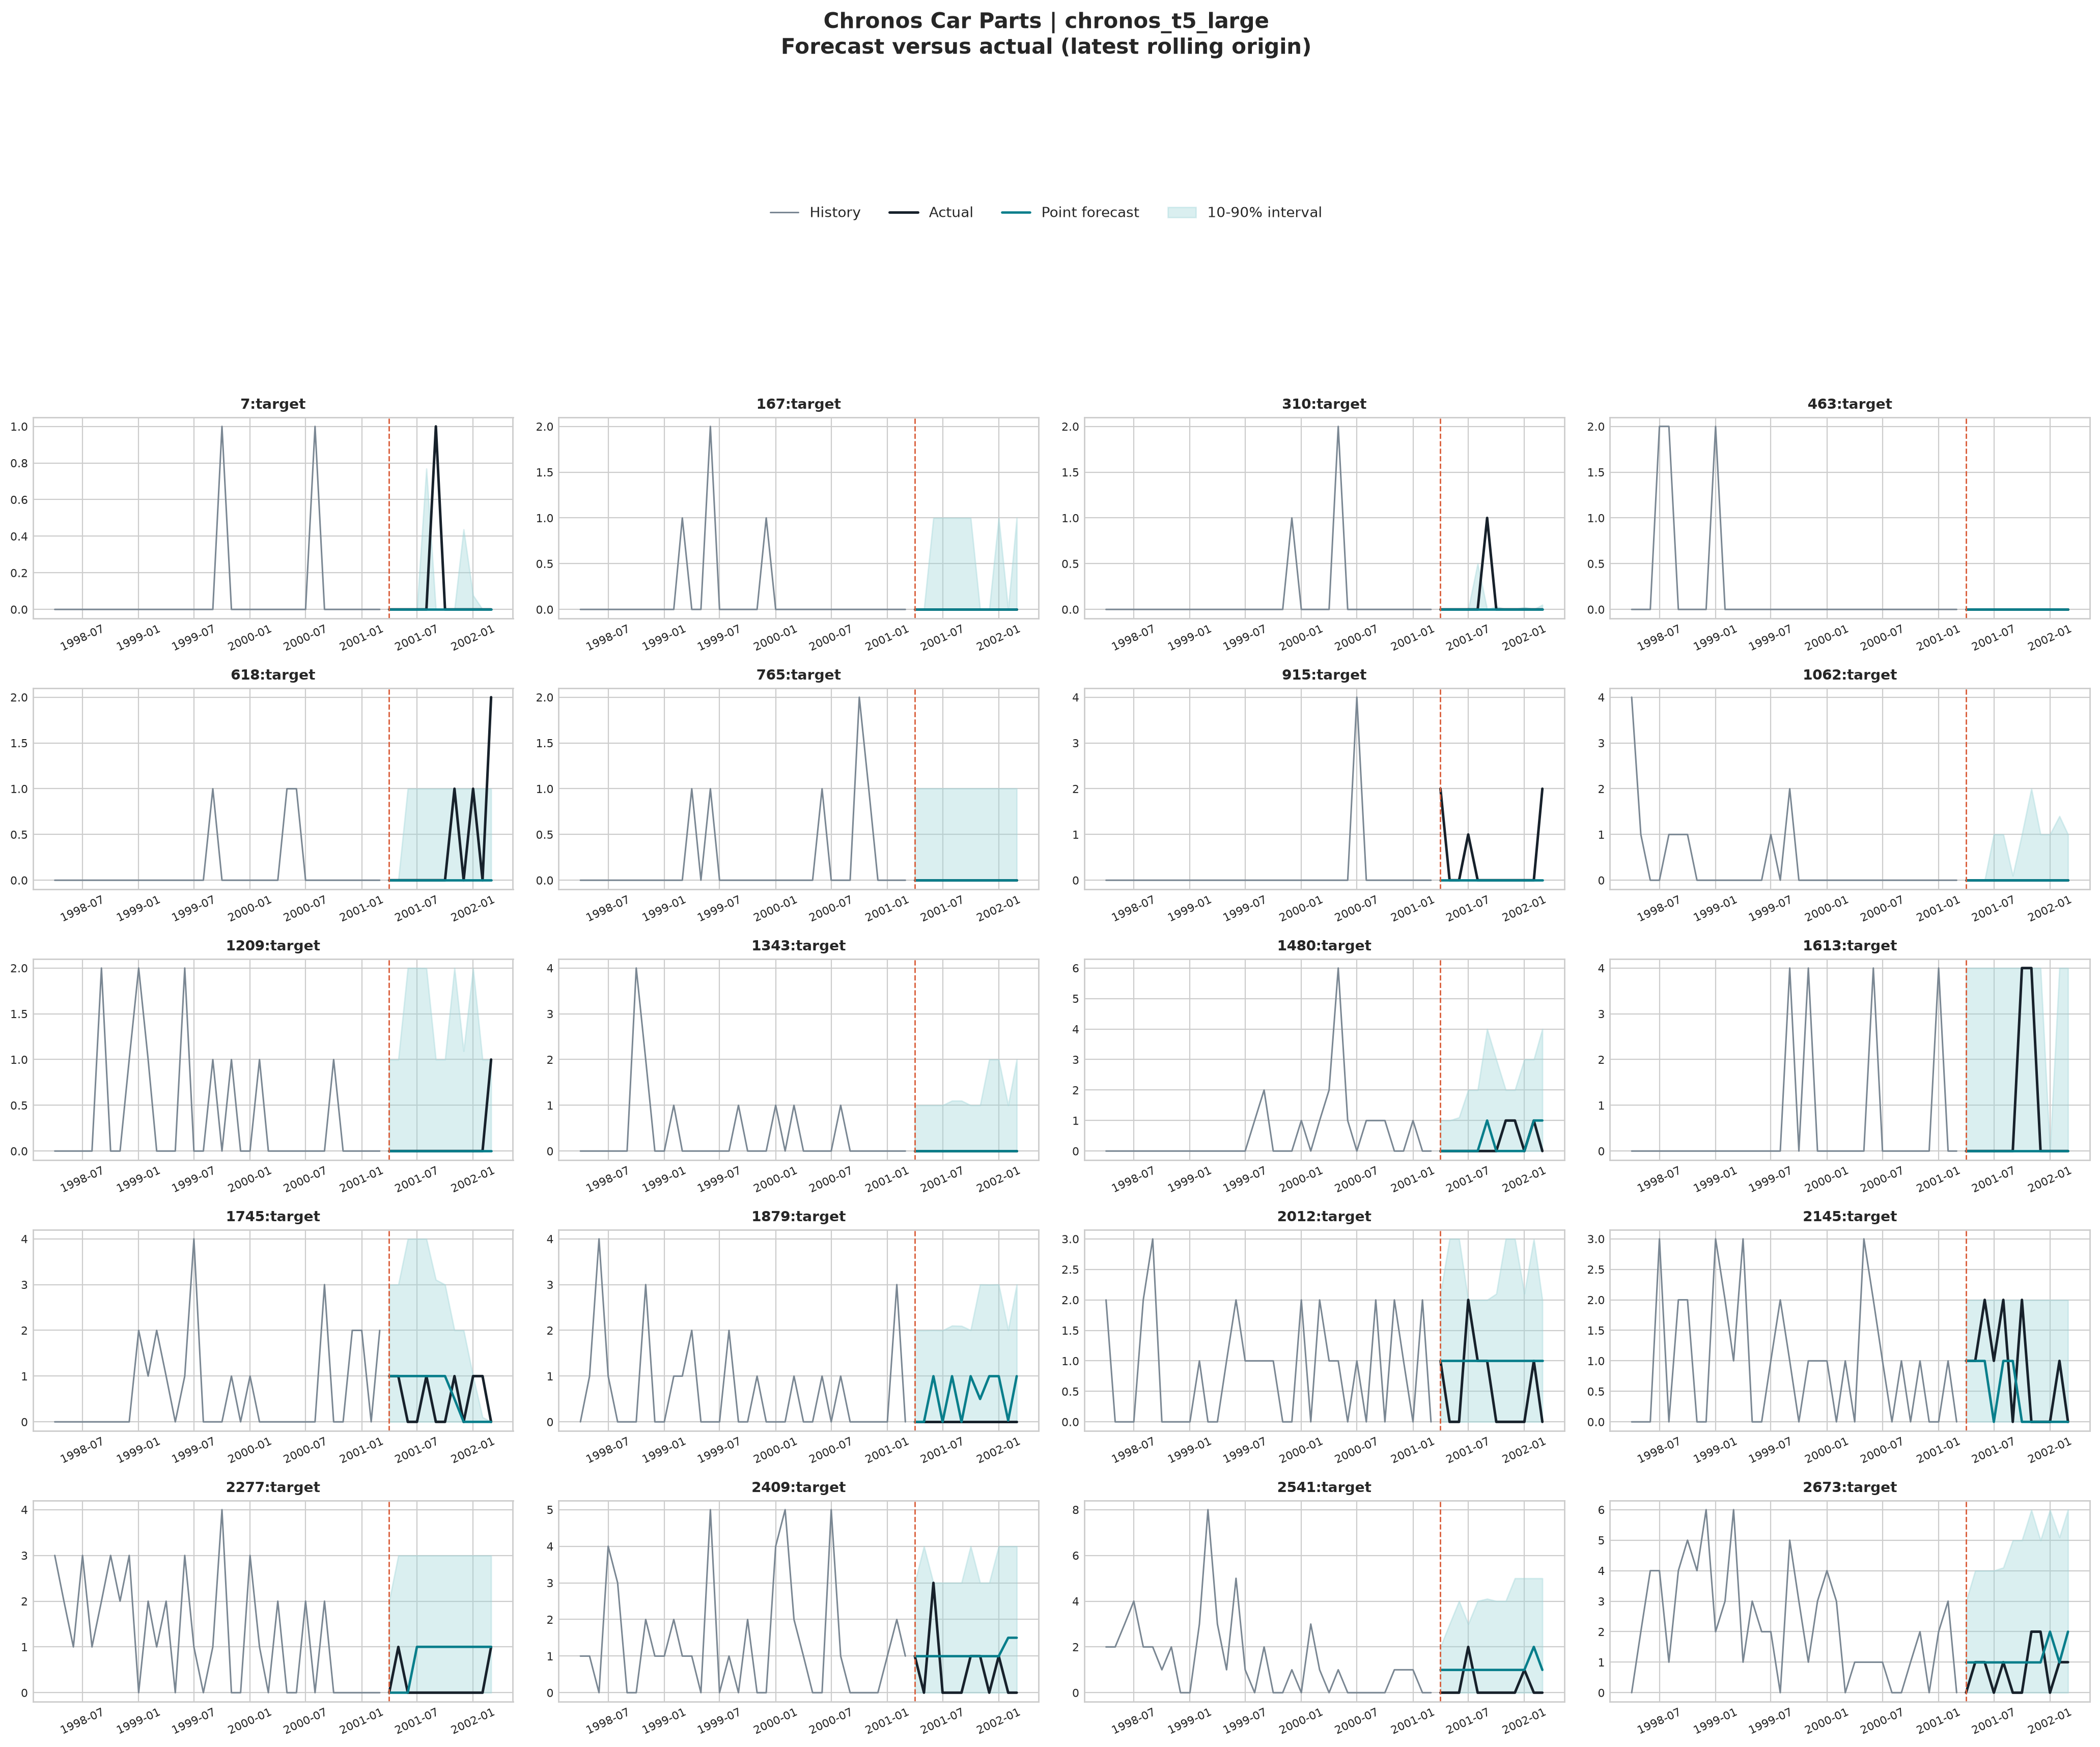
\includegraphics[width=\linewidth,height=0.79\textheight,keepaspectratio]{chronos_car_parts/forecast_vs_actual/chronos_t5_large.png}
\end{frame}

% ------------------------------------------------------------
\begin{frame}{NN5 Weekly --- forecast vs. actual --- Chronos Tiny}
  \centering
  
\includegraphics[width=\linewidth,height=0.79\textheight,keepaspectratio]{chronos_nn5_weekly/forecast_vs_actual/chronos_t5_tiny.png}
\end{frame}

% ------------------------------------------------------------
\begin{frame}{NN5 Weekly --- forecast vs. actual --- TimesFM 2.5}
  \centering
  
\includegraphics[width=\linewidth,height=0.79\textheight,keepaspectratio]{chronos_nn5_weekly/forecast_vs_actual/timesfm_2_5_200m.png}
\end{frame}

% ------------------------------------------------------------
\begin{frame}{NN5 Weekly --- forecast vs. actual --- Moirai 2.0}
  \centering
  
\includegraphics[width=\linewidth,height=0.79\textheight,keepaspectratio]{chronos_nn5_weekly/forecast_vs_actual/moirai_2_0_small.png}
\end{frame}

% ------------------------------------------------------------
\begin{frame}{NN5 Weekly --- forecast vs. actual --- Seasonal Naive}
  \centering
  
\includegraphics[width=\linewidth,height=0.79\textheight,keepaspectratio]{chronos_nn5_weekly/forecast_vs_actual/seasonal_naive.png}
\end{frame}

% ------------------------------------------------------------
\begin{frame}{NN5 Weekly --- forecast vs. actual --- ARIMA(2,1,2)}
  \centering
  
\includegraphics[width=\linewidth,height=0.79\textheight,keepaspectratio]{chronos_nn5_weekly/forecast_vs_actual/arima_2_1_2.png}
\end{frame}

% ------------------------------------------------------------
\begin{frame}{NN5 Weekly --- forecast vs. actual --- AutoARIMA}
  \centering
  
\includegraphics[width=\linewidth,height=0.79\textheight,keepaspectratio]{chronos_nn5_weekly/forecast_vs_actual/auto_arima.png}
\end{frame}

% ------------------------------------------------------------
\begin{frame}{NN5 Weekly --- forecast vs. actual --- Prophet}
  \centering
  
\includegraphics[width=\linewidth,height=0.79\textheight,keepaspectratio]{chronos_nn5_weekly/forecast_vs_actual/prophet.png}
\end{frame}

% ------------------------------------------------------------
\begin{frame}{NN5 Weekly --- forecast vs. actual --- DeepAR}
  \centering
  
\includegraphics[width=\linewidth,height=0.79\textheight,keepaspectratio]{chronos_nn5_weekly/forecast_vs_actual/deepar.png}
\end{frame}

% ------------------------------------------------------------
\begin{frame}{NN5 Weekly --- forecast vs. actual --- Chronos Mini}
  \centering
  
\includegraphics[width=\linewidth,height=0.79\textheight,keepaspectratio]{chronos_nn5_weekly/forecast_vs_actual/chronos_t5_mini.png}
\end{frame}

% ------------------------------------------------------------
\begin{frame}{NN5 Weekly --- forecast vs. actual --- Chronos Small}
  \centering
  
\includegraphics[width=\linewidth,height=0.79\textheight,keepaspectratio]{chronos_nn5_weekly/forecast_vs_actual/chronos_t5_small.png}
\end{frame}

% ------------------------------------------------------------
\begin{frame}{NN5 Weekly --- forecast vs. actual --- Chronos Base}
  \centering
  
\includegraphics[width=\linewidth,height=0.79\textheight,keepaspectratio]{chronos_nn5_weekly/forecast_vs_actual/chronos_t5_base.png}
\end{frame}

% ------------------------------------------------------------
\begin{frame}{NN5 Weekly --- forecast vs. actual --- Chronos Large}
  \centering
  
\includegraphics[width=\linewidth,height=0.79\textheight,keepaspectratio]{chronos_nn5_weekly/forecast_vs_actual/chronos_t5_large.png}
\end{frame}

% ------------------------------------------------------------
\begin{frame}{National Illness --- forecast vs. actual --- Chronos Tiny}
  \centering
  
\includegraphics[width=\linewidth,height=0.79\textheight,keepaspectratio]{external_national_illness/forecast_vs_actual/chronos_t5_tiny.png}
\end{frame}

% ------------------------------------------------------------
\begin{frame}{National Illness --- forecast vs. actual --- TimesFM 2.5}
  \centering
  
\includegraphics[width=\linewidth,height=0.79\textheight,keepaspectratio]{external_national_illness/forecast_vs_actual/timesfm_2_5_200m.png}
\end{frame}

% ------------------------------------------------------------
\begin{frame}{National Illness --- forecast vs. actual --- Moirai 2.0}
  \centering
  
\includegraphics[width=\linewidth,height=0.79\textheight,keepaspectratio]{external_national_illness/forecast_vs_actual/moirai_2_0_small.png}
\end{frame}

% ------------------------------------------------------------
\begin{frame}{National Illness --- forecast vs. actual --- Seasonal Naive}
  \centering
  
\includegraphics[width=\linewidth,height=0.79\textheight,keepaspectratio]{external_national_illness/forecast_vs_actual/seasonal_naive.png}
\end{frame}

% ------------------------------------------------------------
\begin{frame}{National Illness --- forecast vs. actual --- ARIMA(2,1,2)}
  \centering
  \includegraphics[width=\linewidth,height=0.79\textheight,keepaspectratio]{external_national_illness/forecast_vs_actual/arima_2_1_2.png}
\end{frame}

% ------------------------------------------------------------
\begin{frame}{National Illness --- forecast vs. actual --- AutoARIMA}
  \centering
  \includegraphics[width=\linewidth,height=0.79\textheight,keepaspectratio]{external_national_illness/forecast_vs_actual/auto_arima.png}
\end{frame}

% ------------------------------------------------------------
\begin{frame}{National Illness --- forecast vs. actual --- Prophet}
  \centering
  \includegraphics[width=\linewidth,height=0.79\textheight,keepaspectratio]{external_national_illness/forecast_vs_actual/prophet.png}
\end{frame}

% ------------------------------------------------------------
\begin{frame}{National Illness --- forecast vs. actual --- DeepAR}
  \centering
  \includegraphics[width=\linewidth,height=0.79\textheight,keepaspectratio]{external_national_illness/forecast_vs_actual/deepar.png}
\end{frame}

% ------------------------------------------------------------
\begin{frame}{National Illness --- forecast vs. actual --- Chronos Mini}
  \centering
  \includegraphics[width=\linewidth,height=0.79\textheight,keepaspectratio]{external_national_illness/forecast_vs_actual/chronos_t5_mini.png}
\end{frame}

% ------------------------------------------------------------
\begin{frame}{National Illness --- forecast vs. actual --- Chronos Small}
  \centering
  \includegraphics[width=\linewidth,height=0.79\textheight,keepaspectratio]{external_national_illness/forecast_vs_actual/chronos_t5_small.png}
\end{frame}

% ------------------------------------------------------------
\begin{frame}{National Illness --- forecast vs. actual --- Chronos Base}
  \centering
  \includegraphics[width=\linewidth,height=0.79\textheight,keepaspectratio]{external_national_illness/forecast_vs_actual/chronos_t5_base.png}
\end{frame}

% ------------------------------------------------------------
\begin{frame}{National Illness --- forecast vs. actual --- Chronos Large}
  \centering
  \includegraphics[width=\linewidth,height=0.79\textheight,keepaspectratio]{external_national_illness/forecast_vs_actual/chronos_t5_large.png}
\end{frame}

% ------------------------------------------------------------
\begin{frame}{Traffic --- forecast vs. actual --- Chronos Tiny}
  \centering
  \includegraphics[width=\linewidth,height=0.79\textheight,keepaspectratio]{external_traffic/forecast_vs_actual/chronos_t5_tiny.png}
\end{frame}

% ------------------------------------------------------------
\begin{frame}{Traffic --- forecast vs. actual --- TimesFM 2.5}
  \centering
  \includegraphics[width=\linewidth,height=0.79\textheight,keepaspectratio]{external_traffic/forecast_vs_actual/timesfm_2_5_200m.png}
\end{frame}

% ------------------------------------------------------------
\begin{frame}{Traffic --- forecast vs. actual --- Moirai 2.0}
  \centering
  \includegraphics[width=\linewidth,height=0.79\textheight,keepaspectratio]{external_traffic/forecast_vs_actual/moirai_2_0_small.png}
\end{frame}

% ------------------------------------------------------------
\begin{frame}{Traffic --- forecast vs. actual --- Seasonal Naive}
  \centering
  \includegraphics[width=\linewidth,height=0.79\textheight,keepaspectratio]{external_traffic/forecast_vs_actual/seasonal_naive.png}
\end{frame}

% ------------------------------------------------------------
\begin{frame}{Traffic --- forecast vs. actual --- ARIMA(2,1,2)}
  \centering
  \includegraphics[width=\linewidth,height=0.79\textheight,keepaspectratio]{external_traffic/forecast_vs_actual/arima_2_1_2.png}
\end{frame}

% ------------------------------------------------------------
\begin{frame}{Traffic --- forecast vs. actual --- AutoARIMA}
  \centering
  \includegraphics[width=\linewidth,height=0.79\textheight,keepaspectratio]{external_traffic/forecast_vs_actual/auto_arima.png}
\end{frame}

% ------------------------------------------------------------
\begin{frame}{Traffic --- forecast vs. actual --- Prophet}
  \centering
  \includegraphics[width=\linewidth,height=0.79\textheight,keepaspectratio]{external_traffic/forecast_vs_actual/prophet.png}
\end{frame}

% ------------------------------------------------------------
\begin{frame}{Traffic --- forecast vs. actual --- DeepAR}
  \centering
  \includegraphics[width=\linewidth,height=0.79\textheight,keepaspectratio]{external_traffic/forecast_vs_actual/deepar.png}
\end{frame}

% ------------------------------------------------------------
\begin{frame}{Traffic --- forecast vs. actual --- Chronos Mini}
  \centering
  \includegraphics[width=\linewidth,height=0.79\textheight,keepaspectratio]{external_traffic/forecast_vs_actual/chronos_t5_mini.png}
\end{frame}

% ------------------------------------------------------------
\begin{frame}{Traffic --- forecast vs. actual --- Chronos Small}
  \centering
  \includegraphics[width=\linewidth,height=0.79\textheight,keepaspectratio]{external_traffic/forecast_vs_actual/chronos_t5_small.png}
\end{frame}

% ------------------------------------------------------------
\begin{frame}{Traffic --- forecast vs. actual --- Chronos Base}
  \centering
  \includegraphics[width=\linewidth,height=0.79\textheight,keepaspectratio]{external_traffic/forecast_vs_actual/chronos_t5_base.png}
\end{frame}

% ------------------------------------------------------------
\begin{frame}{Traffic --- forecast vs. actual --- Chronos Large}
  \centering
  \includegraphics[width=\linewidth,height=0.79\textheight,keepaspectratio]{external_traffic/forecast_vs_actual/chronos_t5_large.png}
\end{frame}

% ------------------------------------------------------------
\begin{frame}{PSM --- forecast vs. actual --- Chronos Tiny}
  \centering
  \includegraphics[width=\linewidth,height=0.79\textheight,keepaspectratio]{external_psm/forecast_vs_actual/chronos_t5_tiny.png}
\end{frame}

% ------------------------------------------------------------
\begin{frame}{PSM --- forecast vs. actual --- TimesFM 2.5}
  \centering
  \includegraphics[width=\linewidth,height=0.79\textheight,keepaspectratio]{external_psm/forecast_vs_actual/timesfm_2_5_200m.png}
\end{frame}

% ------------------------------------------------------------
\begin{frame}{PSM --- forecast vs. actual --- Moirai 2.0}
  \centering
  \includegraphics[width=\linewidth,height=0.79\textheight,keepaspectratio]{external_psm/forecast_vs_actual/moirai_2_0_small.png}
\end{frame}

% ------------------------------------------------------------
\begin{frame}{PSM --- forecast vs. actual --- Seasonal Naive}
  \centering
  \includegraphics[width=\linewidth,height=0.79\textheight,keepaspectratio]{external_psm/forecast_vs_actual/seasonal_naive.png}
\end{frame}

% ------------------------------------------------------------
\begin{frame}{PSM --- forecast vs. actual --- ARIMA(2,1,2)}
  \centering
  \includegraphics[width=\linewidth,height=0.79\textheight,keepaspectratio]{external_psm/forecast_vs_actual/arima_2_1_2.png}
\end{frame}

% ------------------------------------------------------------
\begin{frame}{PSM --- forecast vs. actual --- AutoARIMA}
  \centering
  \includegraphics[width=\linewidth,height=0.79\textheight,keepaspectratio]{external_psm/forecast_vs_actual/auto_arima.png}
\end{frame}

% ------------------------------------------------------------
\begin{frame}{PSM --- forecast vs. actual --- Prophet}
  \centering
  \includegraphics[width=\linewidth,height=0.79\textheight,keepaspectratio]{external_psm/forecast_vs_actual/prophet.png}
\end{frame}

% ------------------------------------------------------------
\begin{frame}{PSM --- forecast vs. actual --- DeepAR}
  \centering
  \includegraphics[width=\linewidth,height=0.79\textheight,keepaspectratio]{external_psm/forecast_vs_actual/deepar.png}
\end{frame}

% ------------------------------------------------------------
\begin{frame}{PSM --- forecast vs. actual --- Chronos Mini}
  \centering
  \includegraphics[width=\linewidth,height=0.79\textheight,keepaspectratio]{external_psm/forecast_vs_actual/chronos_t5_mini.png}
\end{frame}

% ------------------------------------------------------------
\begin{frame}{PSM --- forecast vs. actual --- Chronos Small}
  \centering
  \includegraphics[width=\linewidth,height=0.79\textheight,keepaspectratio]{external_psm/forecast_vs_actual/chronos_t5_small.png}
\end{frame}

% ------------------------------------------------------------
\begin{frame}{PSM --- forecast vs. actual --- Chronos Base}
  \centering
  \includegraphics[width=\linewidth,height=0.79\textheight,keepaspectratio]{external_psm/forecast_vs_actual/chronos_t5_base.png}
\end{frame}

% ------------------------------------------------------------
\begin{frame}{PSM --- forecast vs. actual --- Chronos Large}
  \centering
  \includegraphics[width=\linewidth,height=0.79\textheight,keepaspectratio]{external_psm/forecast_vs_actual/chronos_t5_large.png}
\end{frame}

% ------------------------------------------------------------
\begin{frame}{Elexon Demand --- forecast vs. actual --- Chronos Tiny}
  \centering
  \includegraphics[width=\linewidth,height=0.79\textheight,keepaspectratio]{official_elexon_demand/forecast_vs_actual/chronos_t5_tiny.png}
\end{frame}

% ------------------------------------------------------------
\begin{frame}{Elexon Demand --- forecast vs. actual --- TimesFM 2.5}
  \centering
  \includegraphics[width=\linewidth,height=0.79\textheight,keepaspectratio]{official_elexon_demand/forecast_vs_actual/timesfm_2_5_200m.png}
\end{frame}

% ------------------------------------------------------------
\begin{frame}{Elexon Demand --- forecast vs. actual --- Moirai 2.0}
  \centering
  \includegraphics[width=\linewidth,height=0.79\textheight,keepaspectratio]{official_elexon_demand/forecast_vs_actual/moirai_2_0_small.png}
\end{frame}

% ------------------------------------------------------------
\begin{frame}{Elexon Demand --- forecast vs. actual --- Seasonal Naive}
  \centering
  \includegraphics[width=\linewidth,height=0.79\textheight,keepaspectratio]{official_elexon_demand/forecast_vs_actual/seasonal_naive.png}
\end{frame}

% ------------------------------------------------------------
\begin{frame}{Elexon Demand --- forecast vs. actual --- ARIMA(2,1,2)}
  \centering
  \includegraphics[width=\linewidth,height=0.79\textheight,keepaspectratio]{official_elexon_demand/forecast_vs_actual/arima_2_1_2.png}
\end{frame}

% ------------------------------------------------------------
\begin{frame}{Elexon Demand --- forecast vs. actual --- AutoARIMA}
  \centering
  \includegraphics[width=\linewidth,height=0.79\textheight,keepaspectratio]{official_elexon_demand/forecast_vs_actual/auto_arima.png}
\end{frame}

% ------------------------------------------------------------
\begin{frame}{Elexon Demand --- forecast vs. actual --- Prophet}
  \centering
  \includegraphics[width=\linewidth,height=0.79\textheight,keepaspectratio]{official_elexon_demand/forecast_vs_actual/prophet.png}
\end{frame}

% ------------------------------------------------------------
\begin{frame}{Elexon Demand --- forecast vs. actual --- DeepAR}
  \centering
  \includegraphics[width=\linewidth,height=0.79\textheight,keepaspectratio]{official_elexon_demand/forecast_vs_actual/deepar.png}
\end{frame}

% ------------------------------------------------------------
\begin{frame}{Elexon Demand --- forecast vs. actual --- Chronos Mini}
  \centering
  \includegraphics[width=\linewidth,height=0.79\textheight,keepaspectratio]{official_elexon_demand/forecast_vs_actual/chronos_t5_mini.png}
\end{frame}

% ------------------------------------------------------------
\begin{frame}{Elexon Demand --- forecast vs. actual --- Chronos Small}
  \centering
  \includegraphics[width=\linewidth,height=0.79\textheight,keepaspectratio]{official_elexon_demand/forecast_vs_actual/chronos_t5_small.png}
\end{frame}

% ------------------------------------------------------------
\begin{frame}{Elexon Demand --- forecast vs. actual --- Chronos Base}
  \centering
  \includegraphics[width=\linewidth,height=0.79\textheight,keepaspectratio]{official_elexon_demand/forecast_vs_actual/chronos_t5_base.png}
\end{frame}

% ------------------------------------------------------------
\begin{frame}{Elexon Demand --- forecast vs. actual --- Chronos Large}
  \centering
  \includegraphics[width=\linewidth,height=0.79\textheight,keepaspectratio]{official_elexon_demand/forecast_vs_actual/chronos_t5_large.png}
\end{frame}

% ------------------------------------------------------------
\begin{frame}{USGS Streamflow --- forecast vs. actual --- Chronos Tiny}
  \centering
  \includegraphics[width=\linewidth,height=0.79\textheight,keepaspectratio]{official_usgs_streamflow/forecast_vs_actual/chronos_t5_tiny.png}
\end{frame}

% ------------------------------------------------------------
\begin{frame}{USGS Streamflow --- forecast vs. actual --- TimesFM 2.5}
  \centering
  \includegraphics[width=\linewidth,height=0.79\textheight,keepaspectratio]{official_usgs_streamflow/forecast_vs_actual/timesfm_2_5_200m.png}
\end{frame}

% ------------------------------------------------------------
\begin{frame}{USGS Streamflow --- forecast vs. actual --- Moirai 2.0}
  \centering
  \includegraphics[width=\linewidth,height=0.79\textheight,keepaspectratio]{official_usgs_streamflow/forecast_vs_actual/moirai_2_0_small.png}
\end{frame}

% ------------------------------------------------------------
\begin{frame}{USGS Streamflow --- forecast vs. actual --- Seasonal Naive}
  \centering
  \includegraphics[width=\linewidth,height=0.79\textheight,keepaspectratio]{official_usgs_streamflow/forecast_vs_actual/seasonal_naive.png}
\end{frame}

% ------------------------------------------------------------
\begin{frame}{USGS Streamflow --- forecast vs. actual --- ARIMA(2,1,2)}
  \centering
  \includegraphics[width=\linewidth,height=0.79\textheight,keepaspectratio]{official_usgs_streamflow/forecast_vs_actual/arima_2_1_2.png}
\end{frame}

% ------------------------------------------------------------
\begin{frame}{USGS Streamflow --- forecast vs. actual --- AutoARIMA}
  \centering
  \includegraphics[width=\linewidth,height=0.79\textheight,keepaspectratio]{official_usgs_streamflow/forecast_vs_actual/auto_arima.png}
\end{frame}

% ------------------------------------------------------------
\begin{frame}{USGS Streamflow --- forecast vs. actual --- Prophet}
  \centering
  \includegraphics[width=\linewidth,height=0.79\textheight,keepaspectratio]{official_usgs_streamflow/forecast_vs_actual/prophet.png}
\end{frame}

% ------------------------------------------------------------
\begin{frame}{USGS Streamflow --- forecast vs. actual --- DeepAR}
  \centering
  \includegraphics[width=\linewidth,height=0.79\textheight,keepaspectratio]{official_usgs_streamflow/forecast_vs_actual/deepar.png}
\end{frame}

% ------------------------------------------------------------
\begin{frame}{USGS Streamflow --- forecast vs. actual --- Chronos Mini}
  \centering
  \includegraphics[width=\linewidth,height=0.79\textheight,keepaspectratio]{official_usgs_streamflow/forecast_vs_actual/chronos_t5_mini.png}
\end{frame}

% ------------------------------------------------------------
\begin{frame}{USGS Streamflow --- forecast vs. actual --- Chronos Small}
  \centering
  \includegraphics[width=\linewidth,height=0.79\textheight,keepaspectratio]{official_usgs_streamflow/forecast_vs_actual/chronos_t5_small.png}
\end{frame}

% ------------------------------------------------------------
\begin{frame}{USGS Streamflow --- forecast vs. actual --- Chronos Base}
  \centering
  \includegraphics[width=\linewidth,height=0.79\textheight,keepaspectratio]{official_usgs_streamflow/forecast_vs_actual/chronos_t5_base.png}
\end{frame}

% ------------------------------------------------------------
\begin{frame}{USGS Streamflow --- forecast vs. actual --- Chronos Large}
  \centering
  \includegraphics[width=\linewidth,height=0.79\textheight,keepaspectratio]{official_usgs_streamflow/forecast_vs_actual/chronos_t5_large.png}
\end{frame}

% ------------------------------------------------------------
\begin{frame}{BLS Macro Indicators --- forecast vs. actual --- Chronos Tiny}
  \centering
  \includegraphics[width=\linewidth,height=0.79\textheight,keepaspectratio]{official_bls_macro/forecast_vs_actual/chronos_t5_tiny.png}
\end{frame}

% ------------------------------------------------------------
\begin{frame}{BLS Macro Indicators --- forecast vs. actual --- TimesFM 2.5}
  \centering
  \includegraphics[width=\linewidth,height=0.79\textheight,keepaspectratio]{official_bls_macro/forecast_vs_actual/timesfm_2_5_200m.png}
\end{frame}

% ------------------------------------------------------------
\begin{frame}{BLS Macro Indicators --- forecast vs. actual --- Moirai 2.0}
  \centering
  \includegraphics[width=\linewidth,height=0.79\textheight,keepaspectratio]{official_bls_macro/forecast_vs_actual/moirai_2_0_small.png}
\end{frame}

% ------------------------------------------------------------
\begin{frame}{BLS Macro Indicators --- forecast vs. actual --- Seasonal Naive}
  \centering
  \includegraphics[width=\linewidth,height=0.79\textheight,keepaspectratio]{official_bls_macro/forecast_vs_actual/seasonal_naive.png}
\end{frame}

% ------------------------------------------------------------
\begin{frame}{BLS Macro Indicators --- forecast vs. actual --- ARIMA(2,1,2)}
  \centering
  \includegraphics[width=\linewidth,height=0.79\textheight,keepaspectratio]{official_bls_macro/forecast_vs_actual/arima_2_1_2.png}
\end{frame}

% ------------------------------------------------------------
\begin{frame}{BLS Macro Indicators --- forecast vs. actual --- AutoARIMA}
  \centering
  \includegraphics[width=\linewidth,height=0.79\textheight,keepaspectratio]{official_bls_macro/forecast_vs_actual/auto_arima.png}
\end{frame}

% ------------------------------------------------------------
\begin{frame}{BLS Macro Indicators --- forecast vs. actual --- Prophet}
  \centering
  \includegraphics[width=\linewidth,height=0.79\textheight,keepaspectratio]{official_bls_macro/forecast_vs_actual/prophet.png}
\end{frame}

% ------------------------------------------------------------
\begin{frame}{BLS Macro Indicators --- forecast vs. actual --- DeepAR}
  \centering
  \includegraphics[width=\linewidth,height=0.79\textheight,keepaspectratio]{official_bls_macro/forecast_vs_actual/deepar.png}
\end{frame}

% ------------------------------------------------------------
\begin{frame}{BLS Macro Indicators --- forecast vs. actual --- Chronos Mini}
  \centering
  \includegraphics[width=\linewidth,height=0.79\textheight,keepaspectratio]{official_bls_macro/forecast_vs_actual/chronos_t5_mini.png}
\end{frame}

% ------------------------------------------------------------
\begin{frame}{BLS Macro Indicators --- forecast vs. actual --- Chronos Small}
  \centering
  \includegraphics[width=\linewidth,height=0.79\textheight,keepaspectratio]{official_bls_macro/forecast_vs_actual/chronos_t5_small.png}
\end{frame}

% ------------------------------------------------------------
\begin{frame}{BLS Macro Indicators --- forecast vs. actual --- Chronos Base}
  \centering
  \includegraphics[width=\linewidth,height=0.79\textheight,keepaspectratio]{official_bls_macro/forecast_vs_actual/chronos_t5_base.png}
\end{frame}

% ------------------------------------------------------------
\begin{frame}{BLS Macro Indicators --- forecast vs. actual --- Chronos Large}
  \centering
  \includegraphics[width=\linewidth,height=0.79\textheight,keepaspectratio]{official_bls_macro/forecast_vs_actual/chronos_t5_large.png}
\end{frame}


\end{document}
